\documentclass[12pt,a4paper]{article}
%\documentclass[11pt]{iopart}

\usepackage[colorlinks=true, linkcolor=black!50!blue, urlcolor=blue, citecolor=blue, anchorcolor=blue]{hyperref}
\usepackage[font=small,labelfont=bf,margin=0mm,labelsep=period,tableposition=top]{caption}

\usepackage[a4paper,top=4cm,bottom=4cm,left=2.5cm,right=2.5cm,bindingoffset=0mm]{geometry}

\usepackage{graphicx}
\usepackage{float}
\usepackage{afterpage}
\usepackage{epsfig,cite}
\usepackage{amssymb}
\usepackage{amsmath}
\usepackage{bm}
\usepackage{dsfont}
\usepackage{multirow}
\usepackage{url}
\usepackage{xcolor}
\usepackage{float}
\usepackage{afterpage}
\usepackage{ulem}

\usepackage{url}
\usepackage{hyperref}

\usepackage{multirow,booktabs,multirow}

%\bibliographystyle{iopart-num}
\bibliographystyle{JHEP}

%%%%%%%%%%%%%%%%%%%%%%%%%%%%%%%%%%%%%%%%%%%%%%%%%%%%%%%%%%%%%

\def\smallfrac#1#2{\hbox{$\frac{#1}{#2}$}}
\newcommand{\be}{\begin{equation}}
\newcommand{\ee}{\end{equation}}
\newcommand{\bea}{\begin{eqnarray}}
\newcommand{\eea}{\end{eqnarray}}
\newcommand{\ei}{\end{itemize}}
\newcommand{\ben}{\begin{enumerate}}
\newcommand{\een}{\end{enumerate}}
\newcommand{\la}{\left\langle}
\newcommand{\ra}{\right\rangle}
\newcommand{\lc}{\left[}
  \newcommand{\tr}{\toprule}
  \newcommand{\mr}{\midrule}
  \newcommand{\br}{\bottomrule}
\newcommand{\rc}{\right]}
\newcommand{\lp}{\left(}
\newcommand{\rp}{\right)}
\newcommand{\as}{\alpha_s}
\newcommand{\aq}{\alpha_s\left( Q^2 \right)}
\newcommand{\amz}{\alpha_s\left( M_Z^2 \right)}
\newcommand{\aqq}{\alpha_s \left( Q^2_0 \right)}
\newcommand{\aqz}{\alpha_s \left( Q^2_0 \right)}
\def\toinf#1{\mathrel{\mathop{\sim}\limits_{\scriptscriptstyle
{#1\rightarrow\infty }}}}
\def\tozero#1{\mathrel{\mathop{\sim}\limits_{\scriptscriptstyle
{#1\rightarrow0 }}}}
\def\toone#1{\mathrel{\mathop{\sim}\limits_{\scriptscriptstyle
{#1\rightarrow1 }}}}
\def\frac#1#2{{{#1}\over {#2}}}
\def\gsim{\mathrel{\rlap{\lower4pt\hbox{\hskip1pt$\sim$}}
    \raise1pt\hbox{$>$}}}       
\def\lsim{\mathrel{\rlap{\lower4pt\hbox{\hskip1pt$\sim$}}
    \raise1pt\hbox{$<$}}}       
\newcommand{\mrexp}{\mathrm{exp}}
\newcommand{\dat}{\mathrm{dat}}
\newcommand{\one}{\mathrm{(1)}}
\newcommand{\two}{\mathrm{(2)}}
\newcommand{\art}{\mathrm{art}}
\newcommand{\rep}{\mathrm{rep}}
\newcommand{\net}{\mathrm{net}}
\newcommand{\stopp}{\mathrm{stop}}
\newcommand{\sys}{\mathrm{sys}}
\newcommand{\stat}{\mathrm{stat}}
\newcommand{\diag}{\mathrm{diag}}
\newcommand{\pdf}{\mathrm{pdf}}
\newcommand{\tot}{\mathrm{tot}}
\newcommand{\minn}{\mathrm{min}}
\newcommand{\mut}{\mathrm{mut}}
\newcommand{\partt}{\mathrm{part}}
\newcommand{\dof}{\mathrm{dof}}
\newcommand{\NS}{\mathrm{NS}}
\newcommand{\cov}{\mathrm{cov}}
\newcommand{\gen}{\mathrm{gen}}
\newcommand{\cut}{\mathrm{cut}}
\newcommand{\parr}{\mathrm{par}}
\newcommand{\val}{\mathrm{val}}
\newcommand{\reff}{\mathrm{ref}}
\newcommand{\Mll}{M_{ll}}
\newcommand{\extra}{\mathrm{extra}}
\newcommand{\draft}[1]{}
% Added by MU 
\def \a{\alpha}
\def \b{\beta}
\def \g{\gamma}
\def \z{\zeta}
\def \t{{\bf T}} % vector of theoretical predictions
\def \c{{\bf c}} % vector of coefficients of theoretical predictions
\def \y{{\bf y}} % vector of experimental data
\def \s{{\bf \sigma}} % experimental covariance matrix
% Added by JR
\def\lapprox{\lower .7ex\hbox{$\;\stackrel{\textstyle <}{\sim}\;$}}
\def\gapprox{\lower .7ex\hbox{$\;\stackrel{\textstyle >}{\sim}\;$}}
\def\half{\smallfrac{1}{2}}
\def\GeV{{\rm GeV}}
\def\TeV{{\rm TeV}}
\def\ap{{a'}}
\def\vp{{v'}}
\def\e{\epsilon}
\def\d{{\rm d}}
\def\calN{{\cal N}}
\def\shat{\hat{s}}
\def\barq{\bar{q}}
\def\qq{q \bar q}
\def\uu{u \bar u}
\def\dd{d \bar d}
\def\pp{p \bar p}
\def\xa{x_{1}}
\def\xb{x_{2}}
\def\xaa{x_{1}^{0}}
\def\xbb{x_{2}^{0}}
\def\smx{\stackrel{x\to 0}{\longrightarrow}}
\def\Li{{\rm Li}}
\numberwithin{equation}{section}
\numberwithin{figure}{section}
\numberwithin{table}{section}
\newcommand{\tmop}[1]{\ensuremath{\operatorname{#1}}}
\newcommand{\tmtextit}[1]{{\itshape{#1}}}
\newcommand{\tmtextrm}[1]{{\rmfamily{#1}}}
\newcommand{\tmtexttt}[1]{{\ttfamily{#1}}}
\usepackage{tabularx}
\newcolumntype{C}[1]{>{\centering\arraybackslash}p{#1}}
\begin{document}
\newgeometry{top=1.5cm,bottom=1.5cm,left=2.5cm,right=2.5cm,bindingoffset=0mm}

%\title[Charting Electron Energy Loss Spectroscopy with machine learning]{Charting the low-loss region in Electron Energy Loss Spectroscopy with machine learning}

%\author{}
%\address{}

%\ead{s.conesaboj@tudelft.nl}
%\vspace{10pt}
%\begin{indented}
%\item[]September 2020
%\end{indented}


\begin{flushright}
Nikhef/2020-022\\
\end{flushright}
\vspace{0.3cm}

\begin{center}
  {\Large \bf Charting the low-loss region in Electron Energy \\[0.3cm] Loss Spectroscopy with machine learning}
\vspace{1.4cm}

Laurien Roest$^{1,2}$, Sabrya E. van Heijst$^{1}$,
  Luigi Maduro$^{1}$,
  Juan Rojo$^{2,3}$,\\[0.2cm] and Sonia Conesa-Boj$^{1}$

\vspace{1.0cm}
 
{\it \small

$^{1}$Kavli Institute of Nanoscience, Delft University of Technology, 2628CJ Delft, The
  Netherlands\\[0.1cm]
$^{2}$Nikhef Theory Group, Science Park 105, 1098 XG Amsterdam, The
  Netherlands \\[0.1cm]$^{3}$Department of Physics and Astronomy, VU,
    1081 HV Amsterdam, The Netherlands

  

}

\vspace{1.0cm}

{\bf \large Abstract}

\end{center}

  Electron energy-loss spectroscopy (EELS) within the
  transmission electron microscope  provides valuable information on the structural, chemical, and electronic properties of materials at the nanoscale.
%
Exploiting the information contained in EEL spectra requires
reliable access to the
low-loss region ($\Delta E\lsim 5$ eV),
where the contribution from the zero-loss peak (ZLP) overwhelms
that from
the inelastic scatterings off the sample.
%
Here we deploy machine learning techniques, inspired in particle physics applications,
to realise a model-independent multidimensional determination of the ZLP
 with a faithful uncertainty estimate.
%
Our method is then used to disentangle
ZLP from the sample contributions in  low-loss EEL spectra acquired
in WS$_2$ nanostructures.
%
This makes possible determining the value and type of the WS$_2$ bandgap
as a function of the underlying crystalline morphology of the nanostructures.

\vspace{0.4cm}
\noindent{\it Keywords:} {\small Transmission Electron Microscopy,
Electron Energy Loss Spectroscopy, Neural Networks, Bandgap, Transition
Metal Dichalcogenides.}\\



%% The words table and figure should be written in full and not abbreviaged to tab. and fig. Do not include ‘eq.’, ‘equation’ etc before an equation number or ‘ref.’ ‘reference’ etc before a reference number.

% Table of contents
\clearpage
\tableofcontents

% General introduction
\section{Introduction}
\label{sec:introduction}

The appreciation for the family of two-dimensional (2D) materials has grown rapidly since the 
first isolation of graphene~\cite{Novoselov:2004}.
%
The properties of these two-dimensional materials are usually very different from their 3D counterparts, 
offering functionalities for novel nanodevices that are not accessible from other heterostructures.
%
The combination of optically active semiconducting layers for light-emitting devices,
the implementation of indirect-to-direct bandgap transition 
materials for flexible electronics, the effect of chemical compositions on many-body instabilities such as
superconductivity~\cite{Novoselov:2016},
%
these are just a few examples of the relevance to exploit the properties of these 2D materials. 
%
However, realizing the full potential of any materials system requires knowing the precise 
electronic, structural and chemical information
at high resolution.

Thanks to recent instrumentation breakthroughs in electron microscopy,
such as electron monochromators~\cite{Terauchi:2005, Freitag:2005} and aberration correctors~\cite{Haider:1998},
it becomes possible to map these properties with unexampled spatial and spectral resolution.
%
Specifically by means of electron energy loss spectroscopy (EELS), it becomes possible to study the local
electronic properties of nanomaterials
down to the atomic scale~\cite{Geiger:1967}, and this way to explore various
important phenomena from the characterisation of bulk and surface plasmons~\cite{Daniels:2003, Schaffer:2008}, 
excitons~\cite{Erni:2005},
phonons~\cite{Ibach:1980}, and inter- and intra-band transitions~\cite{Rafferty:1998},
to the determination of the bandgap energy and the band structure~\cite{Stoger:2008}.

Particulary important information about the material's characteristics can be extracted from studying the
low-loss region of EEL spectra,
defined by electrons that have lost
less than a few eV ($\Delta E\lsim 5$ eV) following their inelastic interactions
with the sample.
%
However, an omnipresent feature called the zero-loss peak (ZLP) dominates
the low-loss region of the spectra. 
%
This narrow, high intensity peak is centered at energy losses
of $\Delta E\simeq 0$, is often asymmetric and its tails extend significantly 
beyond the FWHM. 
%
This peak results from the fact that 
the majority of the incident electron beam will traverse the electron-penetrable sample
either without interactions or scattering only elastically with the 
sample's crystalline lattice, therefore losing little to no energy
and ending up in the ZLP.
%
Since in the low-loss region, the contribution from the ZLP tail
overwhelms those from the inelastic interactions between
the incident electrons and the specimen,
relevant signals of low-loss phenomena such as excitons,
phonons, and intra-band transitions risk being drowned
in the ZLP tail~\cite{Abajo:2010}.
%
An accurate removal of the ZLP
contribution is thus crucial in order to efficiently chart and identify the features
of the low-loss region in EEL spectra. 


Several approaches to ZLP subtraction have been put forward in 
literature~\cite{Rafferty:2000, Erni:2005, Stoger:2008, Egerton:1996,Dorneich:1998, Benthem:2001, Lazar:2003}.
%
These are often based on specific model assumptions about the ZLP properties, specifically
concerning its parametric functional dependence on the electron energy loss $\Delta E$,
from Lorentzian~\cite{Dorneich:1998}
and power laws~\cite{Erni:2005} to more general multiple-parameter functions~\cite{Benthem:2001}.
%
Another approach is based on mirroring the $\Delta E <0$ region of the spectra, assuming
that the $\Delta E>0$ region is fully symmetric~\cite{Lazar:2003}.
%
More recent studies use integrated software applications for background subtraction 
methods~\cite{Egerton:10.1016/S0304-3991(01)00155-3, Held:2020, Granerod:2018, Fung:2020}.
%
These subtraction methods are however affected by three main limitations.
%
Firstly, they rely on specific model assumptions {\it e.g.} with
the choice of a specific fit function, introducing a methodological
bias whose size is difficult to quantify.
%
Secondly, they lack an estimate of the associated uncertainties, which in turn affects
the reliability of any physical interpretations of the low-loss region such as
band gap extraction.
%
Thirdly, methodological choices such as fitting ranges introduce a significant degree of
arbitrariness to the procedure.\\

In this work we bypass these limitations by developing a model-independent strategy
that allows for a multidimensional determination of the ZLP
with a faithful uncertainty estimate.
%
Our approach is based on machine learning (ML) techniques
developed in high-energy physics to study
quark and gluon substructure of protons
particle collisions~\cite{Ball:2008by,Ball:2012cx,Ball:2014uwa,Ball:2017nwa}.
%
This technique is based on the Monte Carlo replica method to construct a probability
distribution in the space of the experimental data (here the ZLP) and to use artificial
neural networks as unbiased interpolators to parametrise the ZLP.
%
The result is
a prediction of the ZLP intensity based on its input variables,
without the need to make specific model assumptions or approximations,
which can be used to subtract its contribution to EEL spectra while
propagating the associated uncertainties.
%
Furthermore, we can extrapolate this ZLP parametrisation to other TEM
operating conditions beyond those included in the training dataset.\\

Our work is divided into two main parts.
%
In the first, we construct a ML model of ZLP spectra taken
in vacuum that is able to accommodate an arbitrary number of input
variables corresponding to different operation settings of the TEM, 
{\it e.g.} exposure time and beam energy
%
We demonstrate how the model describes successfully the
input spectra and we assess its extrapolation for other operating
conditions that were not used for training.

In the second part, we construct a one-dimensional model
of the ZLP as a function of the energy loss from spectra acquired on
tungsten disulfide (WS$_2$) nanostructures~\cite{SabryaWS2}.
%
The resulting subtracted spectra are used to determine
the value and type of the WS$_2$ bandgap
and its dependence on the underlying crystalline morphology, 
and to demonstrate how one can exploit the ZLP-subtracted results
to characterise features arising in the very-low-loss region.

This work is organized as follows.
%
First of all, in Sects.~\ref{sec:tmd} and~\ref{sec:eels}
we discuss the intriguing class of transition metal 
dichalcogenide (TMD) materials, with emphasis on WS$_2$,
and we review the main features of the EELS technique.
%
Sect.~\ref{sec:nn} contains
the fundamentals of neural networks and the principles
of supervised machine learning.
%
In Sect.~\ref{sec:methodology} we describe our machine learning methodology
for the ZLP parametrisation.
%
Sects.~\ref{sec:results_vacuum} and~\ref{sec:results_sample} contain
our results for the ZLP parametrisation for spectra acquired
in vacuum and in samples respectively, which in the latter
case allows us to study the local band structure properties
of the WS$_2$ nanoflowers.
%
Finally in Sect.~\ref{sec:summary} we summarise
and outline possible future developments.
%
Our results have been obtained with an open-source {\sc Python} code,
{\tt EELfitter}, presented in App.~\ref{sec:installation}
together with some installation and usage instructions.


%EELS
\section{Fundamentals of EELS}
\label{sec:eels}

Realizing the full potential of any material requires knowing its 
precise electronic, structural and chemical information at high spacial resolution.
%
One way to achieve this is by means of electron energy loss spectroscopy (EELS).
%
EELS is a method used in combination with 
transmission electron microscopy (TEM), which analyses the 
energy distribution of initially monoenergetic electrons after
they have interacted with a specimen~\cite{Egerton:1996}. 
%
In this chapter, we present an introduction to the basics
of EELS, followed by an overview of energy loss spectra and 
the limitations of the technique.\\

Electron energy loss spectroscopy was developed by James Hillier and R.F. Baker in 
the mid-1940s~\cite{Hillier:1944},
but it was only becoming more widespread in research in the 1990s 
due to improvements in microscope instrumentation. 
%
Since modern instrumentation became widely available in laboratories in the
mid-1990s, the scientific developments regarding electron microscopes grew rapidly.
%
Especially since the introduction of modern aberration correctors
and monochromated electron sources, energy resolutions of 100 meV
or even higher could be achieved~\cite{Rose:2008},
which enabled measurements of single (columns of) atoms. 

Transmission electron microscopy can provide structural information 
with excellent spatial resolution down to atomic dimensions. 
%
These compositional data can be supplemented by chemical information 
from the same specimen region, obtained using analytical techniques
such as EELS.
%
EELS instrumentation is typically incorporated into a scanning
transmission electron microscope (STEM) or in a conventional TEM (c-TEM).
%
These microscope types use high energy electrons, typically 60 - 300 keV, 
to interrogate the sample. 
%
The transmitted electrons are deflected through a uniform magnetic field 
of the order of 0.01 T, generated by an electromagnet with carefully shaped polepieces. 
%
Electrons that scattered inelastically will stray from the central trajectory, 
giving rise to a greater or lesser deflection angle, 
and are sorted and detected according to their energies. 
%
The existence of different kinetic energies thus results in a fringing 
field at the EELS detector.
%
A schematic illustration of a typical EELS setup is shown in the left panel of Fig.~\ref{fig:EELS}.
%

%%%%%%%%%%%%%%%%%%%%%%%%%%%%%%%%%%%%%%%%%%%%%%%
\begin{figure}[H]
    \centering
    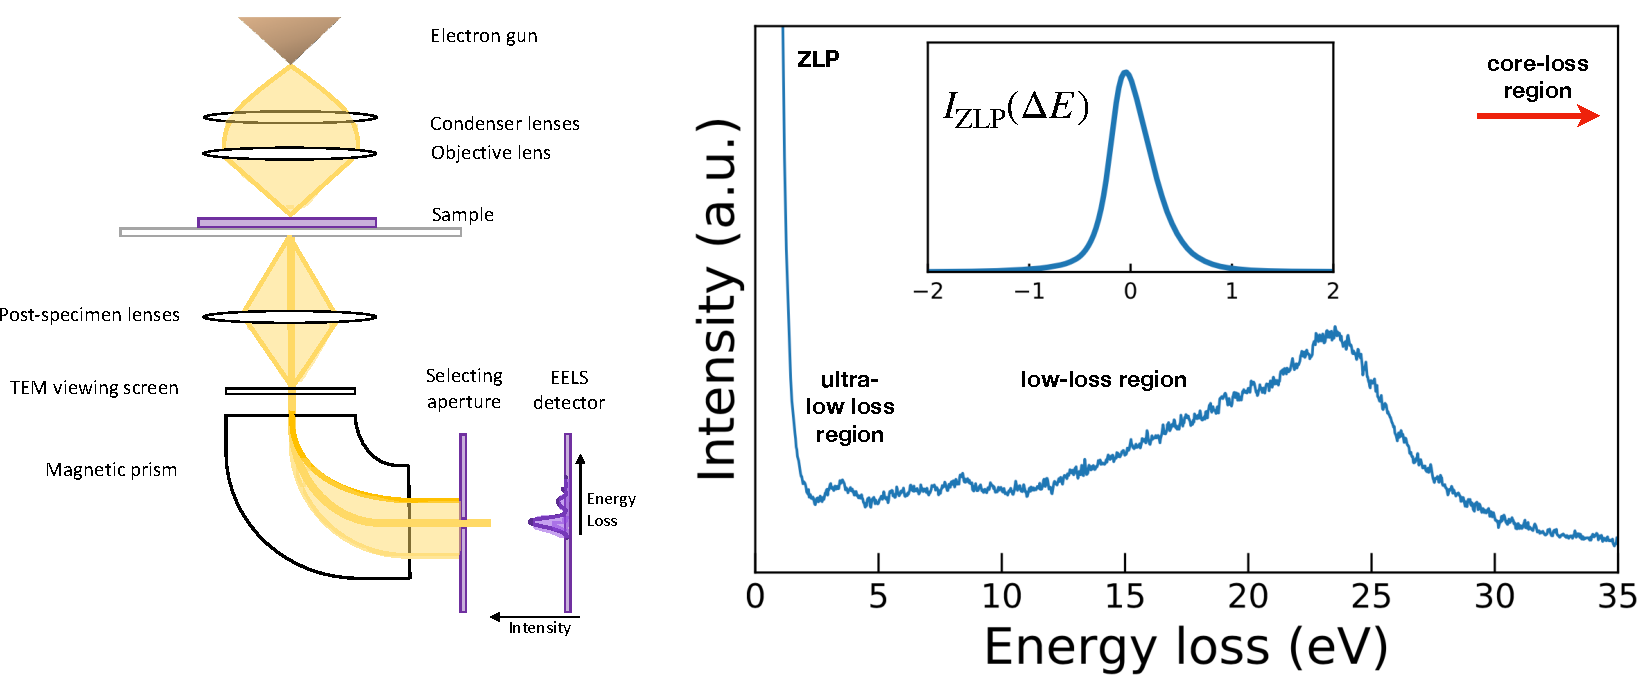
\includegraphics[width=0.97\textwidth]{plots/EELS.pdf}
    \caption{Left: in STEM-EELS, a magnetic
      prism is used to deflect the electron beam after crossing the sample
      so that the distribution of their energy losses $\Delta E$ can be recorded.
      %
      Right: a representative spectrum for $\Delta E \le 35$ eV acquired 
      on a WS$_2$ nanoflower~\cite{SabryaWS2} with
      the inset displaying the corresponding ZLP.
      }
    \label{fig:EELS}
\end{figure}
%%%%%%%%%%%%%%%%%%%%%%%%%%%%%%%%%%%%%%%%%%%%%%%%5

Electron energy loss spectroscopy  provides detailed information about the 
chemical components, bonding, and structure of the specimen.
%
Thanks to recent progress in TEM instrumentation and data acquisition, the EELS technique 
benefits from a combination of both
highly competitive energy (spectral) resolution and spatial resolution.
%
Especially scanning transmission electron microscopy (STEM) equipped with a monochromator 
is extremely useful for high resolution imaging.
%%
The right panel of Fig.~\ref{fig:EELS} displays
a representative EELS spectrum in the region $\Delta E \le 35$ eV, recorded
in one of the WS$_2$ nanostructures presented in~\cite{SabryaWS2},
which will be further discussed later onwards.

\subsection{EEL spectra}
If we are to understand how the features in electron energy loss spectra are produced, 
we must consider how the interaction of the incident electron with the sample 
contributes to the spectrum. 
%
Roughly speaking, EEL spectra can be divided into three main regions.\\

{\bf Zero-loss region.} The first is the zero-loss region, which is centered around $\Delta E=0$
and contains the contributions from electrons that are transmitted without suffering
measurable energy loss.
%
Provided the thickness of the sample is small, the greatest part of the 
incident electron beam transfers through the sample elastically, 
implicating the energy exchange is less than the experimental energy resolution. 
%
A strong and narrow intensity peak around 0 eV loss can be observed called the zero-loss peak (ZLP) or elastic peak. 
The width of the ZLP, typically 0.2-2 eV, reflects the energy distribution of the electron source.

The inset in Fig~\ref{fig:EELS} displays the ZLP, illustrating how nearby $\Delta E\simeq 0$
its magnitude is larger than the contribution from the inelastic interactions
with the sample by several orders of magnitude.
%
This can be explained by the fact that a nucleus is thousands of times more massive than an electron, 
and therefore the energy transfer involved in elastic scattering is usually negligible. 
%
The probability of elastic scattering for a single incident electron 
(per unit solid angle $\Omega$) can to a first approximation be described by 
the differential cross section~\cite{Egerton:1996},
\begin{equation}
    d\sigma_e / d\Omega = \frac{4Z^2/k_0^2T}{(\theta^2 + \theta_0^2)^2}
\end{equation}

where $Z$ is the atomic number, $k_0$ the electron wavenumber, 
and $T$ is not the temperature but the incident electron energy. 
$\theta$ is the scattering angle of the electron of interest, 
and $\theta_0$ represents the angular width of the scattered beam. \\

{\bf Low-loss region.} The second region is the low-loss region or valence region, defined for energy losses
$\Delta E \lsim 50$ eV, which contains information about interactions between the fast incident electrons
and the atoms in the specimen.

The two most fundamental types of collective electronic excitations in solids are plasmons and excitons.
%
In EEL spectra recorded on rather thick specimens, the most prominently observed peaks are plasmon peaks.
%
When an incident electron travels through the crystal lattice, the outer-shell electrons bound to the lattice atoms
are left oscillating, creating a collective of electron excitation modes called  a plasma resonance.
%
This excitation can also be described by means of the creation of a pseudoparticle called a plasmon, 
whose energy depends on the plasmon frequency~\cite{Nerl:2016}.
%
The higher the electron density, the higher the plasmon frequency and therefore the plasmon energy. 
%
Characteristic plasmon-loss peaks appear in the EEL spectra between 5 and 50 eV energy loss, and
can be used to determine the thickness of the specimen, since a higher thickness leads to more
plasmon excitations.

Additionally, the passage of an incident electron can lead to the excitation of a single outer-shell electron.
%
For an insulator or semiconductor, this involves an inter-band transition across the energy bandgap, leaving a hole
behind in the valence band. 
%
The bound state of the electron in the conduction band and electron hole in the valence band is called an exciton.
%
Exciton features appear in the ultra-low-loss region of EEL spectra close to the ZLP, 
characterised by $\Delta E \simeq$ few eV.
%
Here, the contributions of the ZLP and those from the inelastic interactions
with the sample are of the same order of magnitude, and they can be therefore difficultly distinctive~\cite{Abajo:2010}.

When we are dealing with a metal, the higher state can be within the same energy band, corresponding to 
an intra-band transition.
%
Peaks arising from intra-band transition appear very close to the ZLP, with typical energy losses 
below 500 meV.\\

For very thin specimens, the surface and bulk plasmons largely disappear, leaving
interband transitions as the main features in the low-loss regime~\cite{Egerton:1996}.
%
This facilitates the study after the direct bandgap of the material.
%
The  bandgap  refers  to  the  energy  difference between the top of the valence band 
and the bottom of the conduction band and the corresponding peak is expected to appear 
at energy losses where the joint density of states (JDOS) exhibits maxima. 
%
The nature of the bandgap can be either direct or indirect. For direct bandgap materials,
electrons can be directly excited from valence to conduction band. However, 
for indirect band gap materials, a photon or phonon is required to facilitate the transition.
%
For this reason, direct bandgap materials tend to have stronger absorption properties.\\


It has been shown by Bruley and Brown~\cite{Bruley:1987} that for parabolic bands, 
the JDOS probed by the electrons can be described by
\begin{equation}
\label{eq:bandgap}
    \rho(E) = \frac{V}{4\pi^2} \left( \frac{2m^*}{\hbar} \right)^{(3/2)} \alpha \sqrt{E-E_{bg}}
\end{equation}
for a direct band gap, where $m^*$ is the mass of the electrons and holes in the 
valence and conduction band, $E_{bg}$ is the band gap energy and $\alpha$ is the 
convergence angle of the electron beam.
%%
The nature (direct of indirect) and the band gap energy can be deduced 
from the first few eV of the energy-loss function. 
%
From a fit of the band gap onset to Eq.~\ref{eq:bandgap}, 
the value of (1/2) for a direct bandgap switches to (3/2) for an indirect bandgap,
as demonstrated in Fig.~\ref{fig:bandgap}.

\begin{figure}[H]
    \centering
    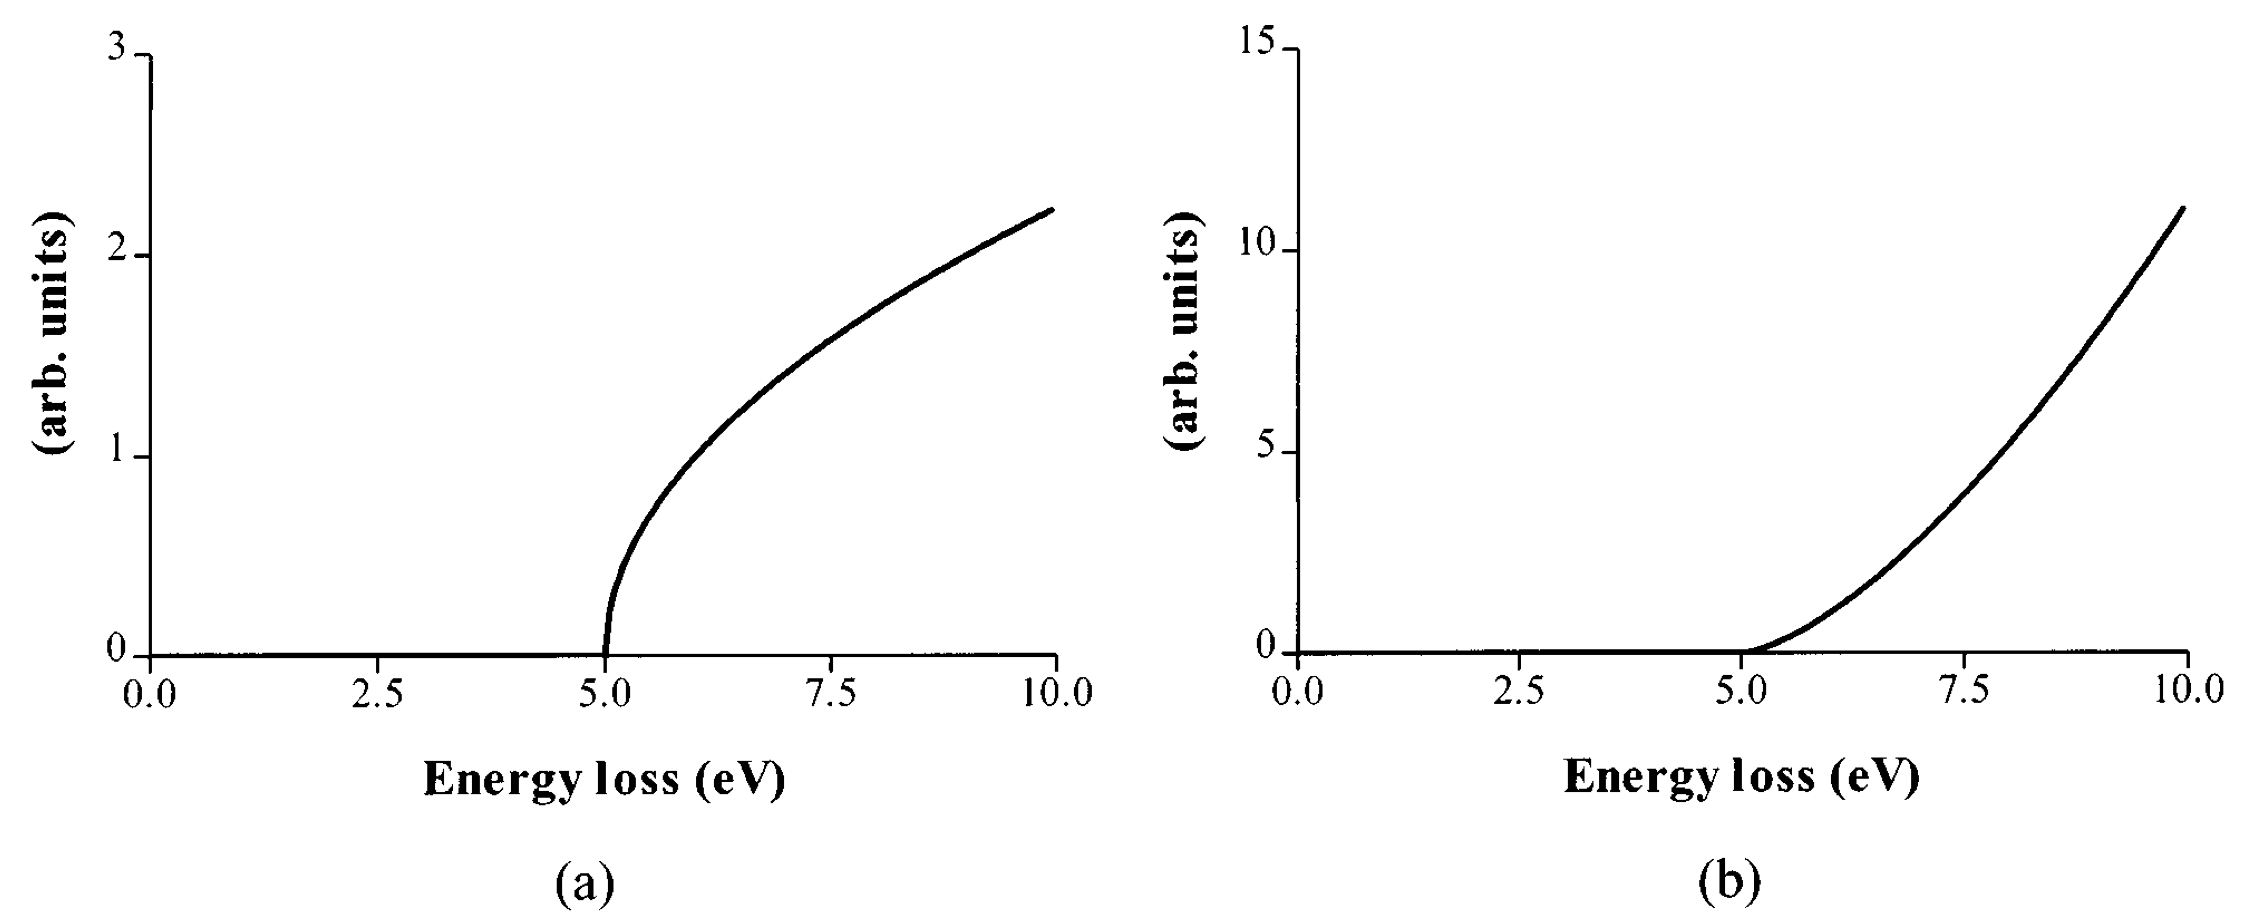
\includegraphics[width=0.8\textwidth]{plots/bandgap.png}
    \caption{Schematic diagrams showing the contributions from the JDOS and matrix elements for (a) direct and (b) indirect transitions. From a fit of the bandgap onset to Eq.~\ref{eq:bandgap}, the power of (1/2) for a direct bandgap switches
    to (3/2) for an indirect transition.
    %
    Retrieved directly from~\cite{Rafferty:1998}.}
    \label{fig:bandgap}
\end{figure}

For materials with a large exciton binding energy, it might happen that the energy exchange
is just barely enough to create an electron-hole pair, but too less to physically separate the electron and hole.
%
We then distinguish between the "optical" and the "electrical" band gap, where the first is the threshold
for the creation of an exciton, while the latter stands for the minimum energy required to create 
an electron-hole pair that is not bound together.
%
The optical and electrical band gap are separated by exactly the binding energy.\\

When we look at features for even lower energy losses in the EEL spectra, $\Delta E \lsim 100$ meV, 
vibrational modes can be revealed. 
%
These are the result of transmitted electrons that generate (and absorb) phonons 
while passing through the crystal. 
%
Phonon energies are of the order $k_bT$ and corresponding energy losses are below $0.1$ eV, 
which requires very high resolution spectroscopy to record it. 
%
Limited vibrational spectroscopy becomes possible in an electron microscope at around 30 meV 
energy resolution. 
%
Vibrational spectroscopy, a field that didn't exist five years ago, includes vibrational mapping, 
analyzing the momentum dependence of vibrational states and determining the local
temperature from the ratio of energy gains to losses~\cite{Krivanek:2009}.\\

{\bf Core-loss region.} The regime for $\Delta E \gsim 50$ eV is the core-loss region,
which provides compositional information
on the elements that constitute the sample. 
%
In this regime, the spectrum shows characteristic features called ionisation edges, 
formed when an inner-shell electron absorbs enough energy from a beam electron 
to be excited to a state above the Fermi level. 
%
The thicker the sample, the more prominent the ionisation edges are 
since multiple scattering events are more common. 
%
In this work however, the focus will be on the low-loss region of EEL spectra, 
therefore we will not go into more detail regarding the core ionisation peaks.


\subsection{Energy resolution}
The energy resolution of an EEL spectrum is determined by several factors. 
%
Firstly, aberrations of the electron spectrometer cause blur of the incoming 
electron beam~\cite{Freitag:2005}. 
%
In general, the spectrometer dispersion becomes worse for higher electron losses,
and therefore the resolution at ionization edges suffers more than close to the
ZLP.
%
Imaging quality can be improved by the implementation of an aberration corrector, 
to cancel the spherical aberration of the objective and condensor lenses. 
%
The energy resolution is then mainly determined by the angular distribution 
provided by the electron beam, usually expressed as the full width at half maximum (FWHM) of the ZLP. 
%
The peak width depends strongly on the electron source. 
An  electron  microscope  equipped  with  a  cold
field emission gun typically has an energy resolution of about 300-800 meV 
under normal operation conditions.  
%
While this width is small compared to the operating voltage of the STEM (usually between 60-300 keV), 
it sets a limit for the energy resolution of EELS and thereby hinders the ability to distinguish 
between peaks separated by less than this value. 
%
Furthermore, for low-loss phenomena such as excitons, 
excitation probabilities can be quite low and these signals can be lost in the tails of the ZLP.\\

The resolution can be drastically improved by implementation of a monochromator 
in the TEM. 
%
In monochromators, a small magnetic prism and energy-selecting slit are installed 
directly after the electron source.
%
This setup essentially works as an energy filter: the incoming electron beam is first dispersed 
before going through a narrow slit, restricting the energy distribution of the incoming electrons. 
%
After compressing it back into the electron probe, the width of the electron beam 
and the tail intensity are greatly reduced.  
%
In a recent studies~\cite{Krivanek:2009}, a monochromated zero-loss peak was obtained 
with a FWHM as small as 4.2 meV and, maybe even more importantly, 
the tail intensity at 20 meV loss has dropped below $10^{-3}$ of its maximum, 
allowing features in the very low-loss region to be resolved. 
%
The improving energy resolution opens new possibilities for accurate measurements
on the bandgap and the 
dielectric function.

Apart from the increase in resolution, another advantage of a monochromated 
electron beam is its symmetric energy distribution. 
%
This directly implies that asymmetries of absorption peaks in the spectrum can 
unambiguously be attributed to the response of the material~\cite{Erni:2005}.
%
The reduction of the energy spread of the incident electron beam often 
comes at the expense of the beam intensity. \\

In Fig~\ref{fig:monochromation}, one can observe the effect of a monochromator 
on the zero-loss peaks of a Schottky field emission microscope in the work of~\cite{Erni:2005}. 
%
Due to thermal broadening, the unfiltered Schottky field-emission source
shows a broad tail at the high-energy side, {\it i.e.} at negative energy loss values.
%
The tails of the monochromated beam are highly symmetrical and the energy dispersion (FWHM)
is greatly reduced.

\begin{figure}[H]
    \centering
    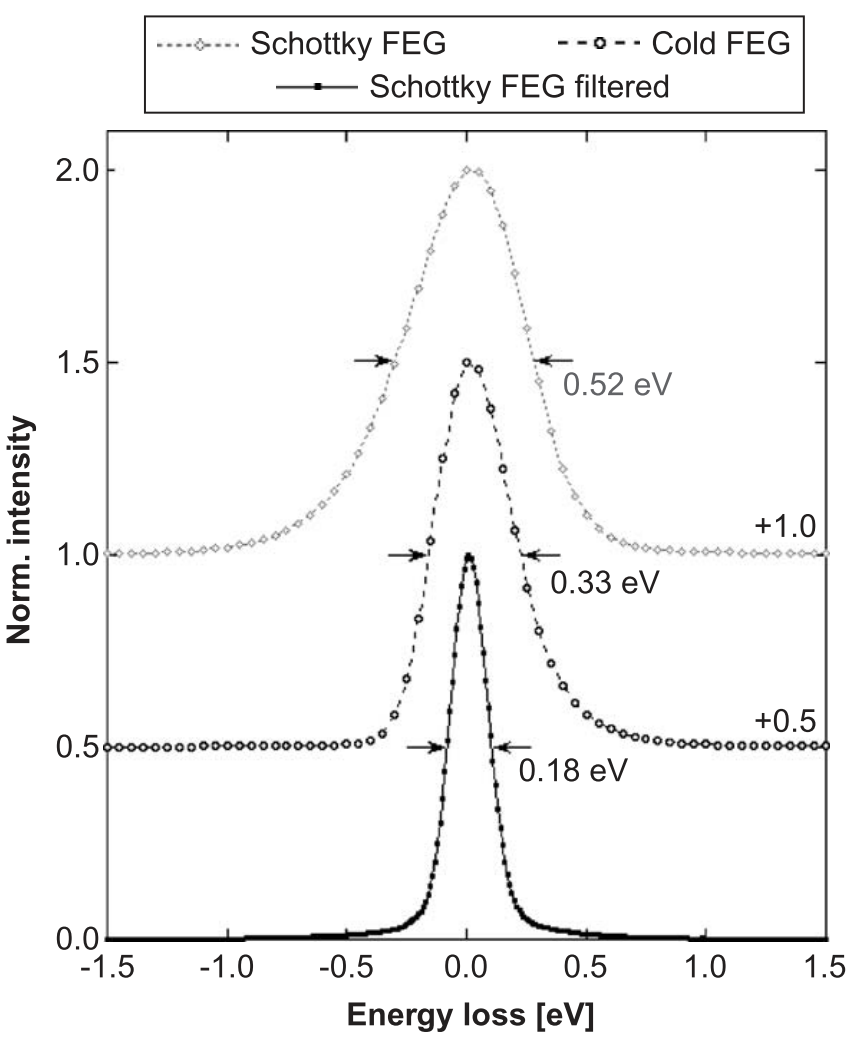
\includegraphics[width=80mm]{plots/monochromator.png}
    \caption{Comparison of the zero-loss peaks of an unfiltered Schottky field emission microscope 
    (200 kV), a cold field-emission microscope (100 kV) and a monochromated electron beam with 
    Schottky field-emission source (200 kV). 
    The second ZLP shows a wider tail at the low-energy side and the tails of the 
    monochromated beam are highly symmetrical. 
    The FWHM indicated in each case provides a measure for the energy resolution.
    %
    Retrieved directly from~\cite{Erni:2005}.}
    \label{fig:monochromation}
\end{figure}


\subsection{ZLP subtraction}
%%%%%%%%%%%
The properties of the ZLP in monochromated EELS depend on the electron energy dispersion,
the monochromator alignment, and the sample thickness~\cite{Park:2008, Stoger:2008}.
%
The first two limitations are already preesent in the absence of a specimen (vacuum operation),
but the third one is associated
to elastic interactions with the sample such as 
phonon excitation, atomic scattering, and exciton losses.
%
This implies that measurements of vacuum EEL spectra can be used for calibration purposes
but not to directly subtract the ZLP from spectra taken on specimens, since their shapes will differ
in general.
%%%%%%%%%%%%%%%


The most important aspect complicating the study of the low-loss regime of EEL spectra 
is the observation of the zero-loss peak, a very intense and ubitiquous feature 
whose right-hand tail suppresses the low-loss features, which results in the loss
of important information within the spectrum.
%
Before analysing the low-loss region of EEL spectra, accurate removal of the
ZLP is crucial. 
%
In the last several years different removal routines for the ZLP were introduced, 
as the increasing energy resolution of the instrumentation would allow for bandgap 
determination by means of VEELS. 
%
The most general suggestion is the subtraction of a fitted ZLP rather than 
using the vacuum recorded ZLP, because a separately recorded peak is always 
different in shape than the one recorded on a sample, due to phonon excitations, 
exciton losses, and broadening at the surface of the sample.
%
Due to the obvious difference in shape between vacuum and in-sample recorded ZLPs, 
direct subtraction of the first on the latter would introduce an extra
source of error. 
%
For this reason, using a fitted ZLP and subtracting it from the EEL spectrum 
is the preferred way to go.
%
Representative examples include the subtraction of a fitted Lorentzian distribution~\cite{Dorneich:1998},
directly subtracting the mirrored left-hand side of the ZLP~\cite{Lazar:2003},
the subtraction of a power-law fit~\cite{Erni:2005}, and the use of a
more general multi-parameter function~\cite{Benthem:2001}.
%
These and several other attempts to model the ZLP distribution 
have had some success at describing the main intensity of the peak, 
but in the tails discrepancies can be as large as several tens of percent~\cite{Bangert:2003}.
%
The standard method for background subtraction of the tails
is to fit a power law to the tails, however this approach is not suitable in
many circumstances~\cite{Hachtel:2018, Tenailleau:1992, Reed:2002, Bosman:2006}.
%
Especially in the very-low-loss region, a simple functional fit completely
removes all intensities belonging to losses within the bandgap energy.
%
More recent studies use integrated software applications for background subtraction 
methods~\cite{Egerton:10.1016/S0304-3991(01)00155-3, Held:2020, Granerod:2018, Fung:2020}.\\

One common flaw of these subtraction methods is the fact that they are often based on specific
model assumptions about the ZLP properties and thereby introduce a methodological
bias which size is difficult to quantify. 
%
This bias arises from assumptions made {\it e.g.} on its functional form, symmetry 
properties, or the fitting range that has been used, all introducing an arbitrariness
to the procedure.
%
Even more importantly, these subtraction methods lack an estimate of the associated uncertainties, 
which in turn affects the reliability of any physical interpretation of features that are observed
in the ZLP-subtracted spectra. 

Developing a model-independent strategy that allows for a determination of the ZLP
with a faithful uncertainty estimate is highly coveted.
%
With the knowledge that the magnitude and shape of the ZLP depend
not only on the specific values
of the electron energy loss $\Delta E$, but also on other operation parameters
of the TEM such as the electron beam energy $E_{\rm b}$, the exposure time
$t_{\rm exp}$, the aperture width and the potential use of a monochromator,
one cannot measure the ZLP for a given operating
condition, for instance a high beam voltage of $E_{\rm b}=200$ keV, and expect to reproduce
the ZLP distribution
associated to different conditions, such as a lower beam voltage of $E_{\rm b}=60$ keV,
without introducing model assumptions.
%
Since it is not possible to compute the dependence of the ZLP on $\Delta E$
and the other operating conditions of the microscope from first principles,
reliance on specific models appears to be unavoidable.
%
Furthermore, even for identical operating conditions, 
the intensity of the ZLP will in general vary due to {\it e.g.} external perturbations 
such as electric or magnetic fields~\cite{Rafferty:2000},
the stability of the microscope and spectrometer electronics~\cite{Kothleitner:2003}, 
the local environment (possibly exposed to mechanical, pressure and temperature fluctuations) 
and spectral aberrations~\cite{Egerton:1996}. 
%
Any model for the ZLP should thus account for this source of uncertainties.



% Review of TMDs and WS2
\section{Transition metal dichalcogenides and WS$_2$}
\label{sec:tmd}

In this work we will apply our machine learning-based method
for describing the ZLP to a novel class of tungsten disulfide (WS$_2$) nanostructures~\cite{SabryaWS2}.
%
WS$_2$ is a transition metal dichalcogenide (TMD) material, which 
belongs to a large family of materials known as two-dimensional (2D) materials or Van der Waals materials.
%
In order to interpret  the obtained EEL spectra later in this work, we first need to 
understand the most important characterics of this class of materials.\\

The appreciation for the family of two-dimensional (2D) materials has grown rapidly since the 
first isolation of graphene almost two decades ago~\cite{Novoselov:2004}.
%
Since then, the family of one-atom-thick crystals has grown with the inclusion of metals, semi-conductors
and insulators. 
%
These materials are named two-dimensional to emphasize their extraordinary thinness: 
TMDs are characterised by the remarkable property of being fully 
functional down to a single atomic layer.
%
The properties of these materials are usually very different from their 3D counterparts
and offer great flexibility for tuning their electronic properties on the nanoscale.

Interestingly, numerous possibilities appear when several 2D crystals are combined in one vertical stacking,
allowing for a much greater number of combinations than traditional growth methods.
%
The nature of the intralayer bonds is mostly covalent, whereas the stacking layers 
are held together by weak van der Waals forces, which allows the crystal to easily cleave 
along the layer surface.
%
Such stackings behave signifcantly different from traditional 3D heterostructures, because each layer 
on itself act as both the interface and the bulk material. 
%
This has great influence on the charge displacements: within each layer, charge transfers are reduced
dramatically, however the mobility can be very large between subsequent layers, which offers
interesting possibilities for engineering the band structure.
%
The relative alignment of neighbouring crystals is therefore of great influence on the physics that can be
observed in such crystals.\\


Over the past few years the exploration of these 2D layered materials
 has developed rapidly. 
 %
 In particular significant attention has been 
 going to transition metal dichalcogenides,
 atomically thin semiconductor of the type $MX_2$, here M is a 
transition metal atom (such as Mo or W) and X is a chalcogen atom (such as S, Se, or Te). 
 %
All TMDs have a hexagonal structure,
with each characteristic monolayer comprising one layer of M atoms 
that is sandwiched between two layers of X atoms.
%
As depicted in Fig.~\ref{fig:stackingtypes}, the two most common coordination phases of the monolayers 
are octahedral and trigonal prismatic, which refers to the coordination of the transition metal atom~\cite{Toh:2017}.
%
The electronic properties of TMDs strongly depends on this coordination,
giving rise to a variety of electronic
 and magnetic properties~\cite{Chhowalla:2013}.
 %
As each individual layer can have any of the two coordinations, 
multi-layered TMDs can have a large variety of stacking types (polytypes), 
of which the most commonly found are defined as 1T, 2H and 3R.
%
In this notation, the digit indicates the number of layers in the unit cell and the
letter stands for trigonal, hexagonal and rhombohedral respectively.

Most of the remarkable electronic and optical properties of TMDs
can be traced back to the underlying periodic arrangements of their layers.
%
For example, the 1T form displays metallic behaviour, 
while both 2H and 3R forms are semiconducting.
%
While nanostructures built upon 2H or 3R crystalline phases have been routinely studied,
knowledge about those based on mixed 2H/3R polytypes is far more limited~\cite{SabryaWS2}.

%%%%%%%%%%%%%%%%%%%%%%%%%%%%%%%%%%%%%%%%%%%%%%%%%%%%%%%%%%%%%%%%%%%%%%%%%%%%%%%
\begin{figure}[H]
    \centering
    \includegraphics[width=0.75\textwidth]{plots/stackings.pdf}
    \caption{The most common coordinations and polytypes of TMD unit cells. 
    %
    Stacking single layers with the  octahedral coordination yields a tetragonal symmetry (1T). 
    %
    The prismatic coordination can yield different stacking symmetries: 
    hexagonal (2H) and rhombohedral (3R).
    %
    Retrieved from~\cite{Toh:2017}}.
    \label{fig:stackingtypes}
\end{figure}
%%%%%%%%%%%%%%%%%%%%%%%%%%%%%%%%%%%%%%%%%%%%%%%%%%%%%%%%%%%%%%%%%%%%%%%%%%%%%%%%%%5


Apart from the dependence on the stacking sequence, 
the properties of this class of materials vary significantly
with their thickness. For instance, MoS$_2$ exhibits an indirect bandgap
in the bulk form which becomes direct at the monolayer level~\cite{Splendiani:2010}.
%
The indirect-to-direct bandgap transition is the main reason for the interest in 
the use of TMDs for flexible electronics: it emphasizes the importance of the
mechanical properties of these materials. 
%
However, it tends to be much more difficult to uniformly deform 2D monolayers
of a material compared to bulk samples, and therefore measuring on 2D systems
can be challenging.
%
TMDs are often combined with other 2D materials like graphene
to make Van der Waals heterostructures, which need to be tuned in order
to function as building blocks for many devices such as LEDs, solar cells, 
transistors, and photodetectors.
%
This research field is still emerging and highly promosing to have a big
impact on future nanotechnology. \\
 
An example of a TMD exhibiting a pronounced dependence on its thickness is 
thungsten disulfide (WS$_2$), with an indirect-to-direct bandgap transition when going
from bulk to bilayer or monolayer form.
%
The effects of this transition are manifested as enhanced
photoluminescence in monolayer WS$_2$, whereas only little emission is observed in
the corresponding bulk form.
%
WS$_2$ adopts a layered structure by stacking atomic layers of S-W-S 
in a sandwich-like configuration, with each monolayer of the trigonal prismatic type (Fig.~\ref{fig:stackingtypes}). 
%
Although the interaction between adjacent layers is a weak Van der Waals 
force, the dependence of the interlayer interaction on the stacking 
order of WS$_2$ is significant.
%
Further applications of this material include storage of hydrogen 
and lithium for batteries~\cite{Bhandavat:2012}.

%%%%%%%%%%%%%%%%%%%%%%%%%%%%%%%%%%%%%%%%%%%%%%%%%%%%%%%%%%%%%%%%%%%%%%%%%%%%%%%
\begin{figure}[h]
    \centering
    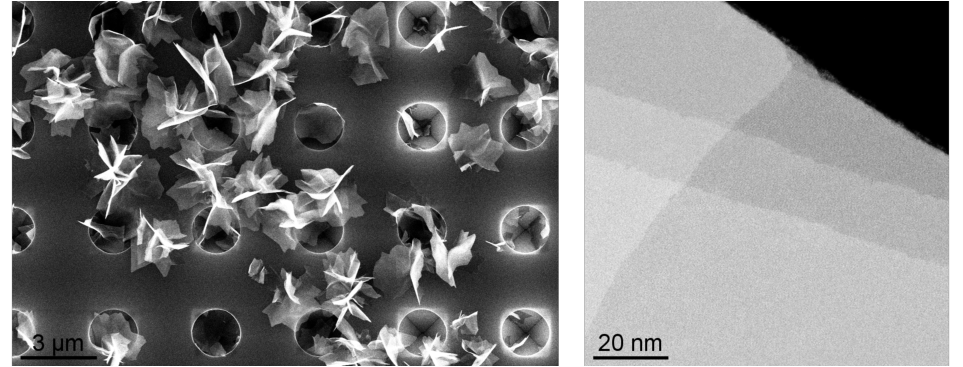
\includegraphics[width=0.8\textwidth]{plots/spectrumimage.pdf}
    \caption{Left: low-magnification TEM image of WS$_2$ nanoflowers
      grown on top of a porous TEM substrate. Right: the magnification of a representative 
      petal of a nanoflower, where the black region corresponds to 
      the vacuum (no substrate) and the difference in contrast indicates terraces of varying thickness.}
    \label{fig:nanoflowers}
\end{figure}
%%%%%%%%%%%%%%%%%%%%%%%%%%%%%%%%%%%%%%%%%%%%%%%%%%%%%%%%%%%%%%%%%%%%%%%%%%%%%%%%%%5

For this work, we have studied specific nanostructures of WS$_2$ called nanoflowers,
which are presented in~\cite{SabryaWS2}. 
%
A low-magnification TEM image of the WS$_2$ nanoflowers is displayed
in the left panel of Fig.~\ref{fig:nanoflowers}.
%
These structures are grown directly on top of a TEM substrate with holes in it. 
%
The right panel shows the magnification of a representative petal of a nanoflower,
where the difference in contrast indicates terraces of varying thickness.
%
Note that the black region corresponds to the vacuum, without
substrate underneath.
%
These WS$_2$ nanoflowers contain areas with different thicknesses, orientations
and crystalline structures, therefore representing an ideal environment to investigate
structural morphology in WS$_2$ with electronic properties at the nanoscale.

What makes it even more interesting is that these nanoflowers exhibit a mixed form of 3R/2H polytypism, 
which is of importance for the interlayer interactions: 
it has been observed that the coexistence of multiple stacking types can complicate
the characterization of the physical properties~\cite{Na:2018}.
%
For example, one possible response of polytypism to electric fields is
 spontaneous electrical polarization, leading to modifications on the 
 electronic band structure and correspondingly on the band gap~\cite{Li:2016}.
 %
Tailoring the specific stacking sequences
represents a powerful strategy to identify and design novel physical properties~\cite{SabryaWS2}.\\

As mentioned before, one of the most interesting properties of TMDs that also
occurs in WS$_2$ is the fact when the material
is thinned down to a single monolayer, its indirect band gap of
$E_{\rm bg}\simeq 1.4$ eV
switches to a direct band gap of approximately $E_{\rm bg}\simeq 2.1$ eV.
%
In general, it has been found that the type and magnitude of the bandgap
of WS$_2$ depends quite sensitively on the crystalline structure and
the number of layers that constitute the material.
%
In Table~\ref{table:bgvalues} we collect
representative results for the determination of the bandgap energy $E_{\rm bg}$
and its type in WS$_2$, obtained by means of different experimental and theoretical techniques.
%
For each reference we indicate separately the bulk results and those
obtained at the monolayer level.
%
We observe that for monolayers, the results for the measured
value of $E_{\rm bg}$ are quite inconsistent, 
reflecting the challenges of its accurate determination.

 
%%%%%%%%%%%%%%%%%%%%%%%%%%%%%%%%%%%%%%%%%%%%%%%%%%%%%%%%%%%%%%%%%%%%%%%%%%%%%%%%%%%%%
\begin{table}[H]
  \small
  \begin{centering}
   \renewcommand{\arraystretch}{1.20}
\begin{tabular}{ccccc}
\br
Reference                       & Thickness & $E_{\rm bg}$ (eV)  & Band gap type  & Technique \\
\mr
{\cite{Braga:2012}} & bulk   & $1.4\pm0.07$            & indirect  & {Gate-voltage dependence}  \\
\mr
\multirow{}{}{\cite{Jo:2014}}                 & ML   & $2.14 $         & direct  & \multirow{}{}{Gate-voltage dependence}        \\
& bulk & $1.40 $    & indirect              \\
\mr

\multirow{}{}{\cite{Gusakova:2007}} & ML   & $2.03\pm0.03$            & direct  & \multirow{}{}{DFT}  \\
& bulk & $1.32\pm0.03 $            & indirect     \\
\mr
\multirow{}{}{\cite{Kam:1982}}                  & ML   & $1.76\pm0.03 $      & direct    & \multirow{}{}{Absorption edge coefficient fitting}         \\
& bulk & $1.35 $          & indirect        \\
\mr
\cite{Shi:2013}                & ML   & $2.21\pm0.3 $         & direct  & Bethe-Salpeter equation (BSE)        \\                 \br                                         
\end{tabular}
\vspace{0.27cm}
\caption{Representative results for the determination of the bandgap energy $E_{\rm bg}$
  and its type in WS$_2$, obtained from a variety of experimental and theoretical techniques.
  %
  For each reference we indicate separately the bulk results and those
  obtained for a monolayers}
    \label{table:bgvalues}
    \end{centering}
\end{table}
%%%%%%%%%%%%%%%%%%%%%%%%%%%%%%%%%%%%%%%%%%%%%%%%%%%%%%%%%%%%%%%%%%%%%%%%%%%%%%%%%%%%%%


% Fundamentals of NN 
\section{Fundamentals of Neural Networks}
\label{sec:nn}

Artificial neural networks (NN) are based on the idea of simulating 
the functioning of neuron connections of the human brain. 
%
This machine learning technique is trained in a fashion similar to 
human learning with the goal to process complex inputs and conclude correct outputs \cite{greplova}.
%
A neural network is defined by a (usually large) number of neurons 
interconnected with strength parameters called weights. 

\begin{figure}[H]
    \centering
    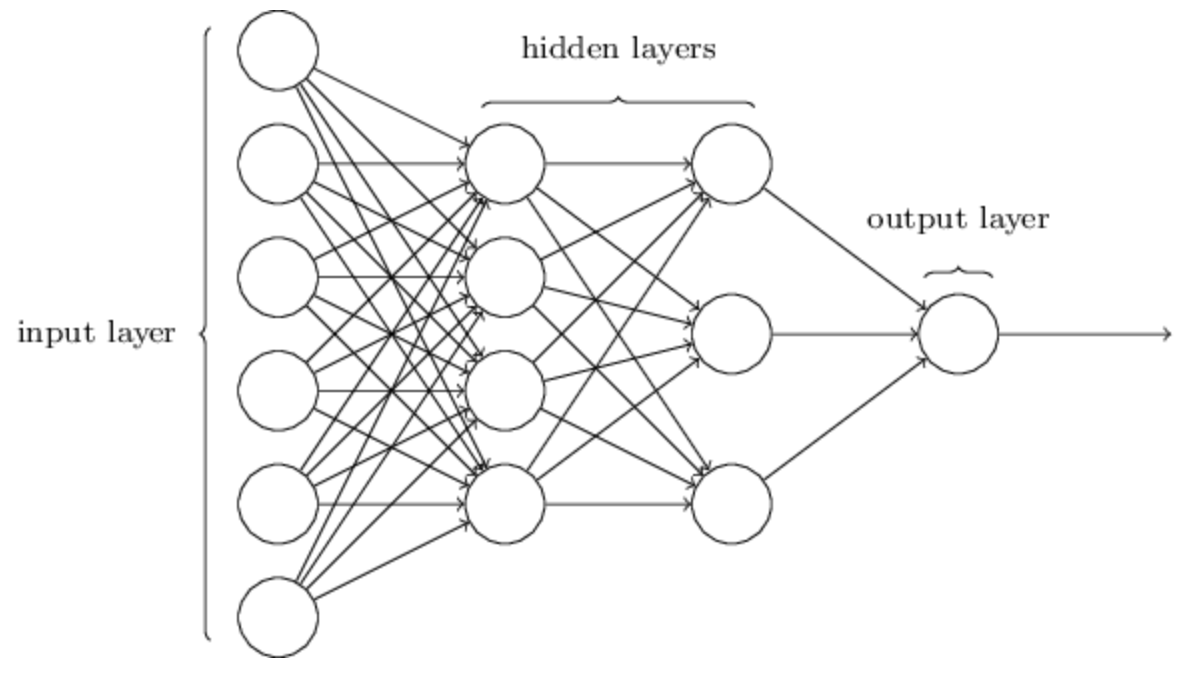
\includegraphics[width=100mm]{plots/nn.png}
    \caption{Schematic representation of a four-layer Neural Network with two hidden layers and one output neuron}
    \label{fig:nn}
\end{figure}

%
Each neuron, represented in the above figure with a circle, 
is connected to a number of neurons in the previous layer and 
its output is the result of an activation function to its inputs:

\begin{equation}
    z = \sum_j w_j x_j + b,
\end{equation}

where $x_j$ are the outputs of the preceding neurons, 
$w_j$ are the corresponding weights and $b$ is the bias (offset) of the neuron. 
%
It is the latter two that will be optimized by training.
A nonlinear activation function $f(z)$ is applied to come to the output value for each neuron; 
this procedure is called forward propagation. 
%
Typical examples for $f(z)$ are the Rectified Linear Unit (ReLU) 
and sigmoid function, as depicted in Fig. \ref{activation}. 
%
Note that these are two often-used, but not the only possible activation functions. 
%
The choice of non-linear activation function influences computational and 
training properties of the neural nets \cite{juan}.
%
For example, choice for the ReLU function ensures absolute positivity. 

\begin{figure}[H]
    \centering
    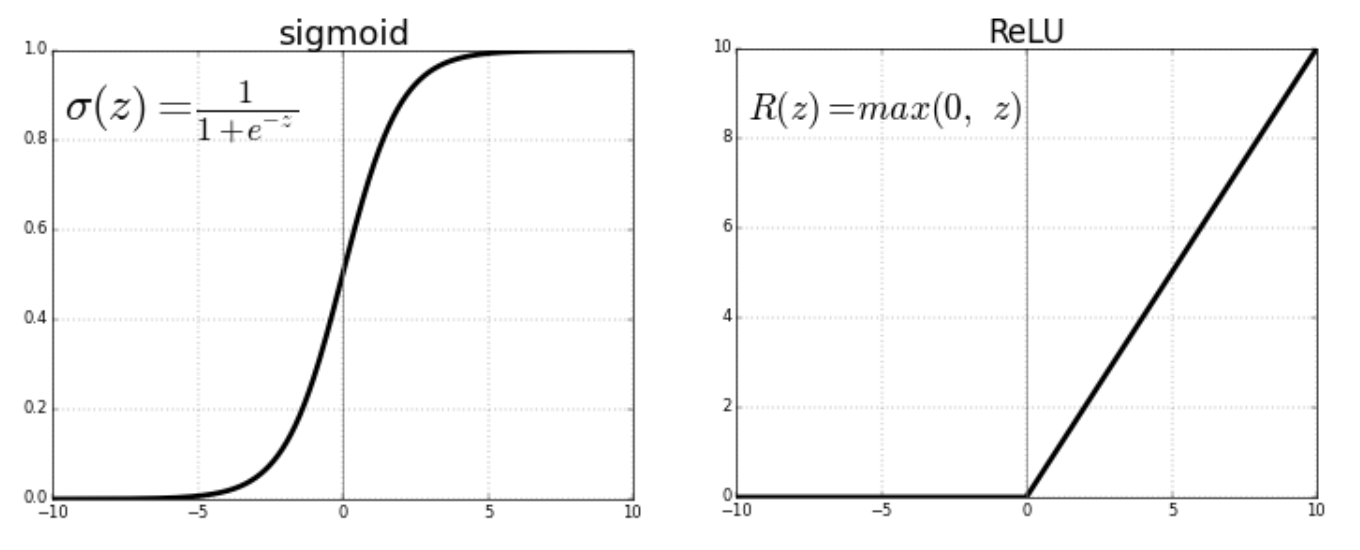
\includegraphics[width=100mm]{plots/f(z).png}
    \caption{Sigmoid (left) and ReLU (right) activation functions. Both approach 0 as $z\rightarrow -\infty$ but note the different behaviour for $z\gg0$. }
    \label{activation}
\end{figure}


For a certain set of inputs \textbf{$x_0$} and a collection of weights and biases $(w^l_j,b^l_j)$, 
with $w^l_j$ being the j-th neuron in the l-th layer.
%
The neural network gives an output $y$ that can be compared to the desired output $y_{target}$. 
%
A cost function $C(y, y_{target})$ is used to quantify how 'far' we are from our desired output, 
and training the algorithm is done by minimizing the cost function with respect to all $(w^l_j,b^l_j)$ of the system. 
%
This minimization is done by means of the gradient descent method, which means 
that after each iteration the weights and biases are adjusted a bit towards 
the minimum of the cost function. 
%
To make this minimization computationally tractable, 
the so-called back-propagation algorithm is being used \cite{hn}, 
allowing us to approximate the derivative of the cost function by averaging over the training set. 
%
All together, training the network relies on the following four fundamental equations:

\begin{align}
\label{eqs3}
\begin{split}
 \delta_j^L &= \frac{\partial C}{\partial a_j^L} f'(z_j^L), 
 \\
 \delta^l &= (w^{l+1} \delta^{l+1}) \odot f'(z^l),
 \\
 \frac{\partial C}{\partial b_j^l} &= \delta_j^l,
 \\
 \frac{\partial C}{\partial w_{jk}^l} &= a_k^{l-1}\delta_j^l.
\end{split}
\end{align}

Here, $\delta_j^l$ is the error and $a_j^l$ the output of neuron $j$ in layer $l$, 
$C$ is the cost, $b$ is the bias and $w$ is the weight of each neuron. 
%
It is the error $\delta_j^L$ that represents the total cost of the network.
%
The last two equations evaluate the gradient of the model parameters 
with the gradient of the cost function. 
%
With this info one can update the model parameters by

\begin{align}
\begin{split}
 b^{l+1} &= b^l - \eta \frac{\partial C}{\partial b^l}
 \\
 w^{l+1} &= w^l - \eta \frac{\partial C}{\partial w^l}
\end{split}
\end{align}
where $\eta$ is the pre-defined learning rate, a measure for the size 
of the step taken with each iteration.
From equations (\ref{eqs3}), one can see that the choice of non-linear 
activation function ($f(z)$) influences the learning of the network. 
%
This can already be deduced from the shape of the functions in Fig.~\ref{activation}: 
since $\sigma$(z) saturates for large inputs $z\gg0$, 
$d\sigma/dz\rightarrow0$ and the network loses sensitivity~\cite{juan}.



We use the definition {\it epoch} for each time that
the entire set of training data is passed forward once through the neural network 
and the network has backpropagated the error and updated all of its parameters
accordingly. 
%
The network needs much more than just one epoch to optimize by means of 
gradient descent, as this is an iterative process. 
%
After each epoch, the performance of the network is evaluated by calculating
the error ($ \delta_j^L$) on the training data and the weights and biases
are adjusted accordingly.
%
As the number of epochs increases, the network parameters are adjusted
repeatedly and where the network was first underfitting the inputs at
the beginning, at a certain moment it goes to optimal fitting,
before it enters the overfitting regime.
%
Several methods can be applied to determine the optimal stopping point
of the network, that is, to find the moment at which the network is
neither under-, nor overfitting the training data. 
%
One of such is splitting the total set of experimental data into two sets:
the training dataset is the one we use to train the model, usually
80\% of the total set.
%
The other 20\% is what we call the validation set and it is used to provide
an unbiased evaluation of the model fit on the training set. 
%
This split ratio is common for models with a moderate number of hyperparameters:
increasing the size or increasing the tunability of the model usually goes with increasing the share of the
validation set. 
%
The validation subset is left out of the training set on purpose and the model
can not learn on this data points.
%
After each epoch, the total performance of the
system can be validated by feeding this subset to the network and calculating
the total error on this data.
%
Tracing the cost function on both the training and the validation set 
gives insight in if the network is overfitting the training data.
First, both the training and validation error will be decreasing, 
but at a certain point the network will start overfitting and the
validation error slowly starts to increase. 
%
The optimal stopping point is defined as the global minimum of the 
error of the validation sample, computed over a large fixed number of 
iterations.
%
A typical progress of the training and validation error over the 
course of the optimization can be observed in Fig.~\ref{fig:cost}.

\begin{figure}[H]
    \label{fig:costs}
    \centering
    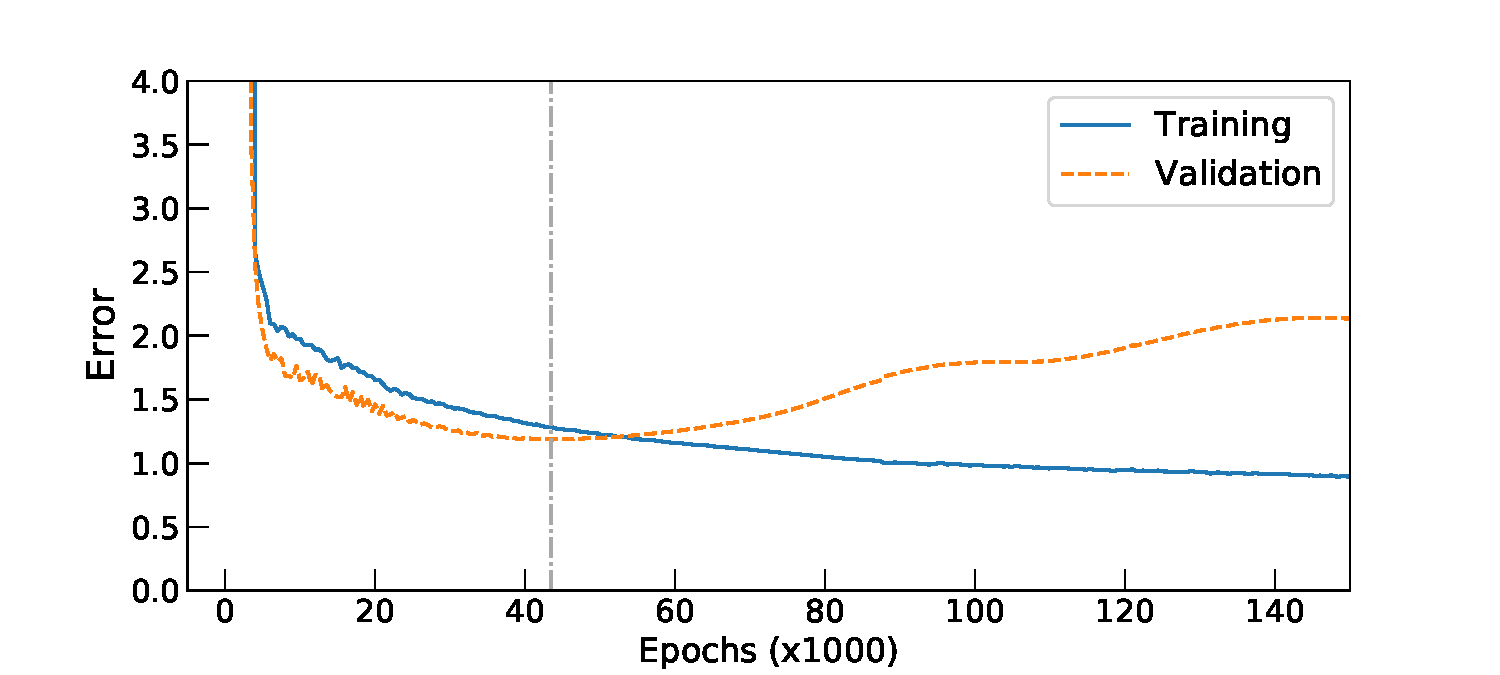
\includegraphics[width=150mm]{plots/train_val_error.pdf}
    \caption{Progress of both the training and validation error over 
    one training session as a function of the number of epochs. 
The optimal stopping point is where the validation error is at
its absolute minimum, here after 43,500 epochs.}

\end{figure}

%
Once the optimal network parameters have been determined and stored, 
the network can be used to
make predictions on any set of inputs. 








% Discuss the methodology that we are going to use
%%%%%%%%%%%%%%%%%%%%%%%%%%%%%%%%%%%%%%%%%%%%%%%%%%%%%%
\section{Neural network determination of the ZLP}
%%%%%%%%%%%%%%%%%%%%%%%%%%%%%%%%%%%%%%%%%%%%%%%%%%%%%
\label{sec:methodology}

In this section we present our strategy to parametrise, predict and subtract 
the zero loss peak by means of machine learning.
%
As mentioned in the introduction, our strategy will be inspired by the 
NNPDF method~\cite{Rojo:2018qdd} originally developed in the context of high-energy physics
for studies of the quark and gluon substructure of the proton~\cite{Gao:2017yyd}.
%
The NNPDF approach has been successfully applied, among others, to
the determination of
unpolarised~\cite{DelDebbio:2007ee,Ball:2008by,Ball:2012cx,Ball:2014uwa,Ball:2017nwa}
and polarised parton distributions functions of protons, nuclear
parton distributions~\cite{AbdulKhalek:2019mzd,AbdulKhalek:2020yuc}, and the
fragmentation functions of partons into neutral and charged
hadrons~\cite{Bertone:2017tyb,Bertone:2018ecm}.
%
Neural networks benefit from the ability to parametrise 
multidimensional input data with arbitrarily non-linear dependencies:
even with a single hidden layer, a neural network can reproduce arbitrary 
functional dependencies provided it has a large enough number of neurons.
%
We can therefore apply a similar procedure for the determination of the
functional dependence of the ZLP intensity. 

We note that recently several applications of machine learning
to transmission electron microscopy analyses 
in the context of material science have been
presented, see {\it e.g.}~\cite{Gordon:2020, Zhang:2019, Jany:2017, Ziatdinov:2017,10.1145/2834892.2834896,doi:10.1021/acsnano.7b07504,cite-key}.
%
Representative examples
include the automated identification
of structural information at the atomic scale~\cite{10.1145/2834892.2834896} 
and the extraction of chemical information
and defect classification~\cite{doi:10.1021/acsnano.7b07504}.
%
For the readout of EEL spectra specifically, 
machine learning has been put forward for the prediction
of spectral features in the core-loss regime~\cite{Kiyohara:2018}.
%
To the best of our knowledge, this is the first time that neural networks are used as 
unbiased background-removal interpolators and that they are used combined with 
Monte Carlo sampling to construct an estimate of the model uncertainties.\\

In this section, we discuss the parametrisation of the ZLP in terms of neural networks.
%
The ultimate goal is to create a model that is able to predict the contribution $I_{\rm ZLP}$
in the total intensity profile of any EEL spectrum recorded over a specimen, 
and subsequently to subtract this distribution from the spectrum to isolate the inelastic
scattering contributions.
%
In order to do so, we first need to develop a model that is able to predict the general
shape of the zero loss peak as a function of its input parameters. 
%
For this we use in-vacuum zero loss peak recordings, which function as a baseline to 
create this generic, multidimensional model.
%
In this regard we also
explain the Monte Carlo replica method, which is used to estimate and propagate the
uncertainties from the input data to the model predictions.
%
After this we move on to the training strategy on sample spectra: 
we explain how the method is modified to use it on spectra recorded over
WS$_2$ specimens and how one can select the hyper-parameters that appear in the model.


\subsection{ZLP parametrisation}
\label{sec:parametrisation}

Without any loss of generality, we can decompose recorded the intensity profile
in any EEL spectrum as
\be
\label{eq:IeelTot}
I_{\rm EEL}(\Delta E) =I_{\rm ZLP}(\Delta E) + I_{\rm inel}(\Delta E) \, ,
\ee
where $\Delta E$ is the measured electron energy loss; $I_{\rm ZLP}$ is the zero loss
distribution arising both from instrumental origin and from elastic interactions; and
$I_{\rm inel}(\Delta E)$ contains the contributions from the electrons that have undergone
inelastic scattering with the specimen. 
%
It is the latter contribution that we're particularly interested in, but in order 
to get hold of it we need to disentangle it from the zero loss contribution.
%
As shown by the representative example of Fig.~\ref{fig:EELS}, there are two limits
for which one can straightforwardly separate the two contributions.
%
The first region is for sufficiently high energy losses, where
$I_{\rm ZLP}$ vanishes and $I_{\rm EEL} \to I_{\rm inel}$.
%
Secondly, in the region close to zero, all emission can be associated to
the ZLP such that $I_{\rm EEL}\to  I_{\rm ZLP}$.
%
It is the region in between that is of particular interest, 
the ultra-low-loss region where $I_{\rm ZLP}$ and $I_{\rm inel}$
become of comparable order of magnitude.

Our goal is to construct a parametrisation of $I_{\rm ZLP}$ based on artificial
neural networks, which we denote by $I_{\rm ZLP}^{\rm (mod)}$, which allows us to
extract the relevant inelastic contribution by subtracting the
contribution of the ZLP from the total EEL spectra:
\be
\label{eq:ZLPseparation}
I_{\rm inel}(\Delta E) \simeq I_{\rm EEL}(\Delta E) - I_{\rm ZLP}^{\rm (mod)}(\Delta E) \,.
\ee
Isolating $I_{\rm inel}$ from the total spectrum makes us able to exploit 
the physical information contained in the low-loss region.
%
Crucially, we aim toestimate and propagate all the relevant sources of uncertainty associated
both to the input data and to methodological choices. 
%
This helps us to verify our results and to separate lucky findings from real insights.\\

As discussed in Sect.~\ref{sec:eels}, the ZLP depends both
on the value of the electron energy loss $\Delta E$ as well as on the operating
conditions of the microscope, such as the electron beam energy $E_b$ and the exposure time
$t_{\rm exp}$.
%
Therefore we want to construct a multidimensional model which can theoretically take any number of relevant variables
as input, in order to reproduce the predicted zero loss peak.
%
This means that in general Eq.~(\ref{eq:ZLPseparation}) can be written as
\be
I_{\rm inel}(\Delta E) = I_{\rm EEL}(\Delta E, E_{b},t_{\rm exp}, \ldots) - I_{\rm ZLP}^{\rm (mod)}(\Delta E, E_{b},t_{\rm exp}, \ldots) \, ,
\ee
where we note that the subtracted spectrum $I_{\rm inel}(\Delta E)$ should depend only on the energy loss, but not on the microscope parameters.
%
Ideally, the ZLP model should be able to accomodate as many input variables as possible.
%
The output of the ZLP model is parametrised by means of multi-layer feed-forward artificial neural networks.
This means that the predicted zero loss peak intensity can be expressed as 
\be
\label{eq:ZLPmodelNN}
I_{\rm ZLP}^{\rm (mod)}(\Delta E, E_{b},t_{\rm exp}, \ldots)  = \xi^{(n_l)}_1(\Delta E, E_{b},t_{\rm exp}, \ldots) \, ,
\ee
where $\xi^{(n_l)}_1$ is the activation state of the single output neuron in the last
of the $n_l$ layers of the network. Here the $n_I$ inputs are the variables $\{ \Delta E, E_{b},t_{\rm exp}, \ldots \}$
that represent the relevant information about the operating conditions during the recording of the spectra.
%
Note that for this work, we have used spectra recorded under the known conditions $\{ \Delta E, E_{b},t_{\rm exp}\}$. 
%
This set of inputs could potentially be extended by including extra variablesm, 
{\it e.g.} arperture width, abberation correction and temperature. 
%
The neural network is then trained by means of supervised learning and non-linear regression on these  
$n_I$ inputs, using the known corresponding ZLP intensities $I_{\rm ZLP}^{\rm (mod)}$ as training outcomes. 
%
Each iteration, the weights and thresholds of this neural network model are optimized
from the minimization of the error on this training dataset.\\

The number of hidden layers and neurons that is optimal is very task depenend and
should therefore be decided arbitrarily, 
there is no general rule of thumb. 
%
We have chosen to use an $n_I$-10-15-5-1 architecture with three hidden layers, wich corresponds to a total
number of 289~(271) free parameters for $n_I=3$~($n_I=1$) to be optimised.
%
However, we have verified that results are fairly independent of this exact choice:
predictions on the training data did not change significantly when the architecture 
was increased by a factor of two.

  
%%%%%%%%%%%%%%%%%%%%%%%%%%%%%%%%%%%%%%%%%%%%%
\begin{figure}[t]
    \centering
    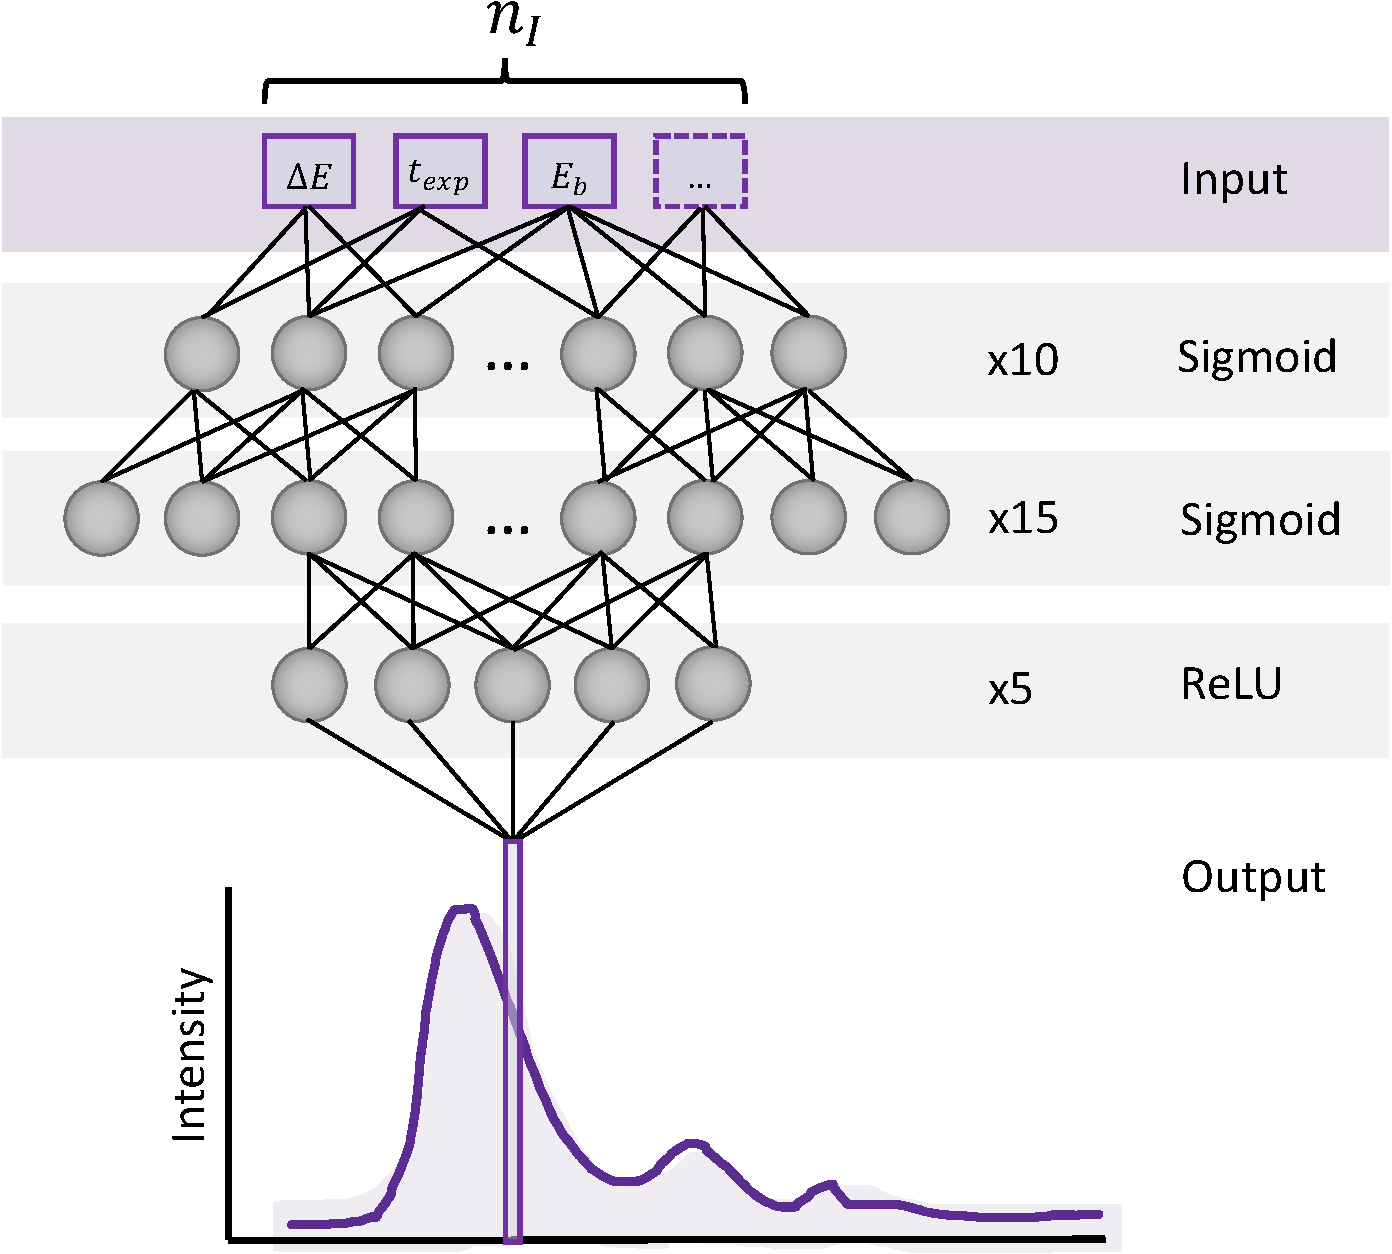
\includegraphics[width=99mm]{plots/architecture.pdf}
    \caption{Schematic representation of our ML model for the ZLP, Eq.~(\ref{eq:ZLPmodelNN}).
      %
      The input is an $n_I$-dimensional array containing $\Delta E$ and other
      operation variables of the microscope such as $E_b$ and $t_{\rm exp}$.
      %
      The output is the predicted value of the intensity of the zero-loss peak
      distribution associated to those specific input variables.
      %
      The architecture is chosen to be $n_I$-10-15-5-1, with sigmoid activation functions
      in all layers except for a ReLU in the output neuron.
    }
    \label{fig:architecture}
\end{figure}
%%%%%%%%%%%%%%%%%%%%%%%%%%%%%%%%%%%%%%%%%%%%%%%%%

A schematic representation of this model
is displayed in Fig.~\ref{fig:architecture}.
%
 The input is an $n_I$ array containing $\Delta E$ and the rest of
 operation variables of the microscope, and
 the output is the value of the intensity of the ZLP distribution
 associated to those input variables.
 %
 We use a sigmoid activation function for the three hidden layers and a ReLU
 for the final one.
 %
 The choice of ReLU for the final layer guarantees that our model for the ZLP
 is positive-definite, as required by general physical considerations: the intensity
 count can never be smaller than zero.
 %
 We have adopted a redundant architecture to ensure that the ZLP parametrisation
 is sufficiently flexible, which means that this way we guarantee that
 the network can over-fit on the training inputs.
 %
 However, the final results should be evaluated before the network starts overfitting,
 as described in Sect.~\ref{sec:neuralnetworks}. 
 %
 This means that we need to define a suitable regularisation strategy, which 
 will be explained later onwards in Sect.~\ref{sec:training}.



\subsection{Uncertainty propagation}
\label{sec:uncertaintypropagation}

We discussed in Sect.~\ref{sec:eels} how
even for EEL spectra taken at identical operating conditions of the microscope,
in general the resulting ZLP intensity profiles will be different.
%
Also, the input data can be described by a large number of different neural 
network configurations, each with a different functional form of $I_{\rm ZLP}^{(\rm mod)}$
but representing the data equally well.
%
The Monte Carlo replica method can be used to estimate these two sources of 
uncertainties, introduced by the experimental data and the methodology,
and to propagate them to physical predictions.
%
The basic idea is twofold:
first, it is useful to represent problems with a possibility of non-gaussian errors
through the use of their central values and uncertainties, which are obtained from a Monte Carlo sample
as their averages and standard deviations.
%
Second, when a problem requires a reconstruction of discrete sampling without making assumptions on its 
functional form, neural networks are useful to work as unbiased interpolators. 
%
It is the combination of both techniques that explains the use of neural networks to separate a smooth
signal from background signals, while the MC samples handles the fluctuations within the data.

%%%%%%%%%%%%%%%%%%%%%%%%%%%%%%%%%%%%%%%%%%%%%%%
\begin{figure}[h]
    \centering
    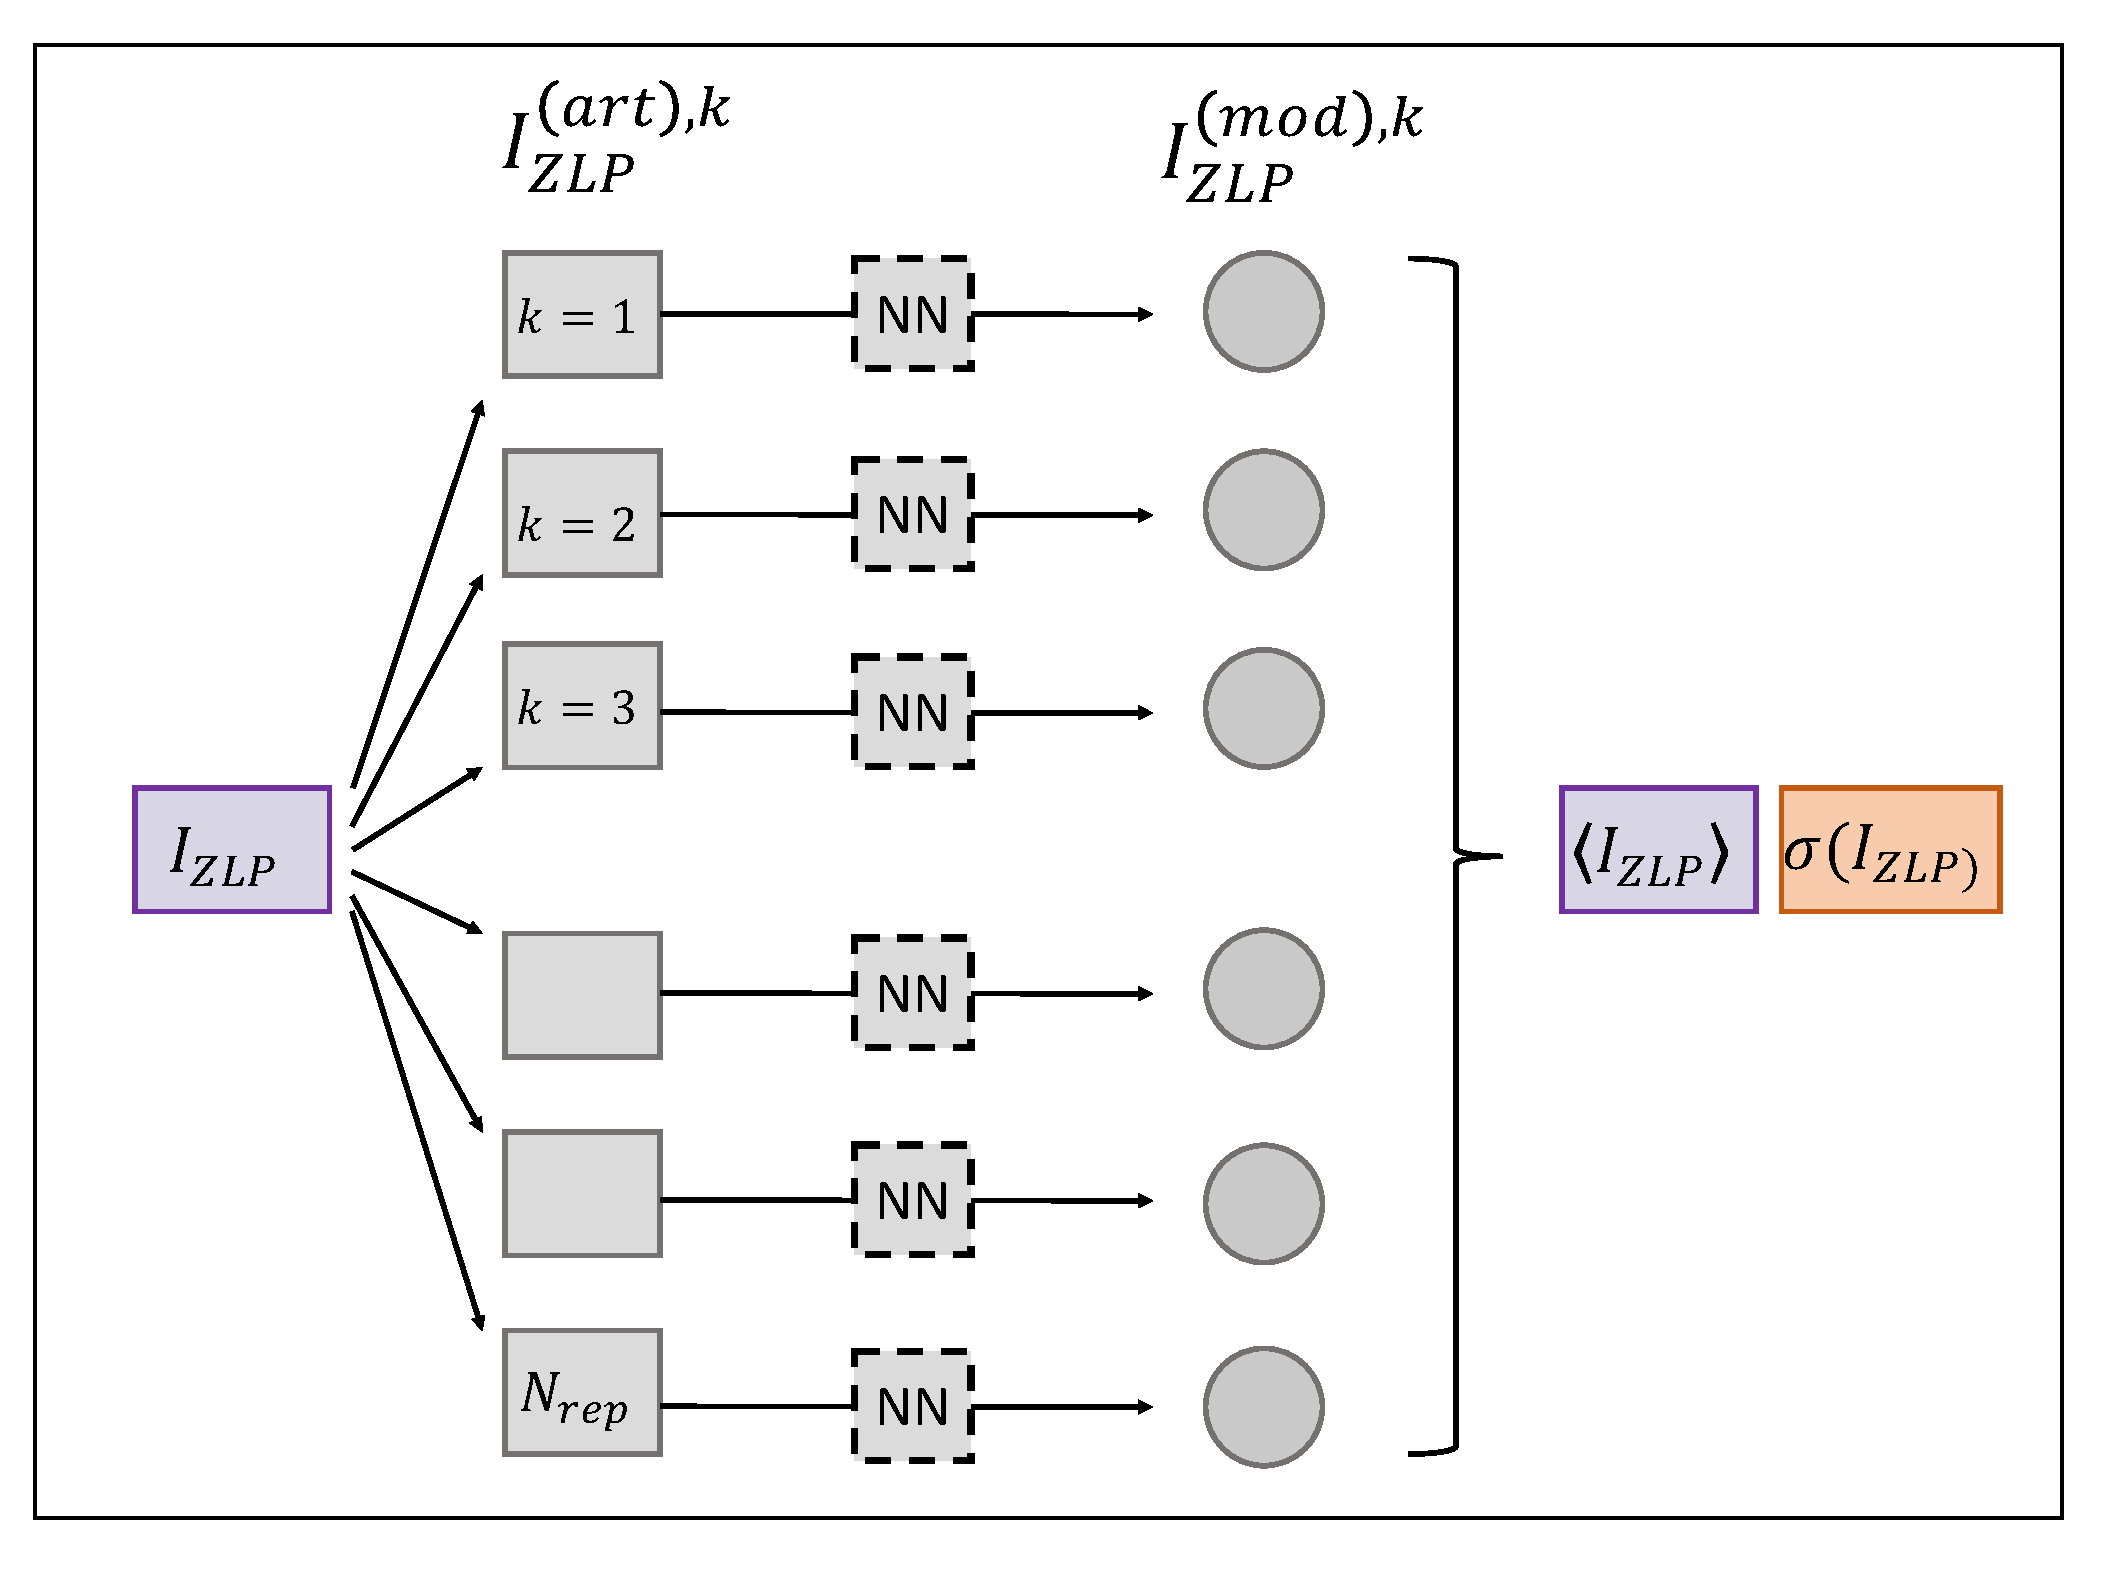
\includegraphics[width=0.7\textwidth]{plots/MCscheme.pdf}
    \caption{Representation of the Monte Carlo replica strategy. From the original set of training data,
    an ensemble of replicas is created from the experimental central values and uncertainties. 
    On each replica, an individual neural network is trained and a ZLP parametrisation is obtained.
    The total set of predictions is then used to calculate physical observables from the corresponding
    central values and uncertainties.}
    \label{fig:MCscheme}
\end{figure}
%%%%%%%%%%%%%%%%%%%%%%%%%%%%%%%%%%%%%%%%%%%%%%%%5

The MC strategy is schematically summarized in figure \ref{fig:MCschema} and it involves two stages.
In the first, we generate an ensemble of replicas of the original training set. 
%
Then, each replica
is passed through an individual neural network, which thereby outputs a parametrisation of the ZLP.
%
Any physical observables can be calculated over the set of computed ZLP distributuions.\\

Let us assume that we have $n_{\rm dat}$ independent measurements of the ZLP intensity, 
so our training dataset contains $n_{\rm dat}$ data points, all with different combinations of input parameters. 
%
The collective of inputs are given as $\{z_i\}$:
\be
I^{\rm (exp)}_{{\rm ZLP},i}\lp \{ z_i  \}\rp = I^{\rm (exp)}_{{\rm ZLP},i}\lp  \Delta E_i, E_{b,i}, t_{\rm exp,i},\ldots \rp
\,, \quad i=1,\ldots,n_{\rm dat} \, .
\ee

The Monte Carlo method is based on the generation
of a large number $N_{\rm rep}$ of Monte Carlo replicas of these original data points
by means of a multi-Gaussian distribution, where we use the central values and covariance matrices
from the input measurements. 
%
The strategy of the generation of Monte Carlo replicas goes as follows: we create for each original data point
($I^{\rm (exp)}_{{\rm ZLP},i}$) an ensemble of artificial pseudo points (replicas): 
\be
\label{eq:MCreplicaGen}
  I_{{\rm ZLP},i}^{{\rm (art)}(k)}  =  I^{\rm (exp)}_{{\rm ZLP},i} + r_i^{({\rm stat},k)}\sigma_i^{\rm (stat)}
  + \sum_{j=1}^{n_{\rm sys}} r_{i,j}^{({\rm sys},k)} \sigma_{i,j}^{\rm (\rm sys)} \,, \quad \forall i
  \,, \quad k=1,\ldots,N_{\rm rep} \,.\,\, \,
  \ee
  where $\sigma_i^{\rm (stat)}$ and $\sigma_{i,j}^{\rm (\rm sys)}$ represent the statistical
  and systematic uncertainties (the latter divided into  $n_{\rm sys}$ fully point-to-point correlated
  sources) and $\{r_i^{(k)}\}$ are Gaussianly distributed random numbers.
  %
In the end, each $k$-th replica contains exactly
as many data points as the original set.

In our case we have no information on experimental correlations betweem the measurements and
for this reason we assume that there is only one single source of point-by-point systematic
uncertainty, which is uncorrelated. 
%
  Should in the future correlations became available, it would be straightforward to extend
  our model to that case.
%
In other words, to each data point we associate an individual uncertainty and we 
discard covariances between datapoints, which means that we drop the last term in Eq.~(\ref{eq:MCreplicaGen})
and it reduces to
\be
\label{eq:MCreplicaGen2}
  I_{{\rm ZLP},i}^{{\rm (art)}(k)}  =  I^{\rm (exp)}_{{\rm ZLP},i} + r_i^{({\rm stat},k)}\sigma_i^{\rm (stat)}
\ee

These statistical errors on the training data can be derived by means of what is called
equal width discretization (EWD) and it works as follows.
%
The input measurements will be composed in general on subsets of EEL
spectra taken with identical operation conditions.
%
For example, we have one specific set of $N_{sp}$ spectra all recorded with 
the same exposure time and beam energy. 
%
Since the range of $\Delta E$ over which the spectra have been recorded
is usually not the same in each case, first of 
we uniformise a common binning in $\Delta E$ with $n_{\rm dat}$ entries.
%
Then we evaluate the total experimental uncertainty in one of these bins as
\be
\sigma_i^{\rm (exp)} = \lp \frac{1}{N_{\rm sp}-1} \sum_{l=1}^{N_{\rm sp}}
\lp I_{{\rm ZLP},i}^{ ({\rm exp}),l}  - \la I_{{\rm ZLP},i}^{ ({\rm exp})}\ra_{N_{\rm sp}} \rp \rp^{1/2} \, ,\,
i=1,\ldots, n_{\rm dat} \, ,
\ee
that is, $\sigma_i^{\rm (exp)}$ is the standard deviation in bin $i$ calculated over the $N_{\rm sp}$ spectra.
%
This uncertainty is separately evaluated for each set of microscope operation conditions
for which data available.
%
The value of the number of generated MC replicas, $N_{\rm rep}$, should be chosen such that the set of replicas 
models accurately the probability distribution of original training data.
%
%%%%%%%%%%%%%%%%%%%%%%%%%%%%%%%%%%%%%%%%%%%%%%%
\begin{figure}[t]
    \centering
    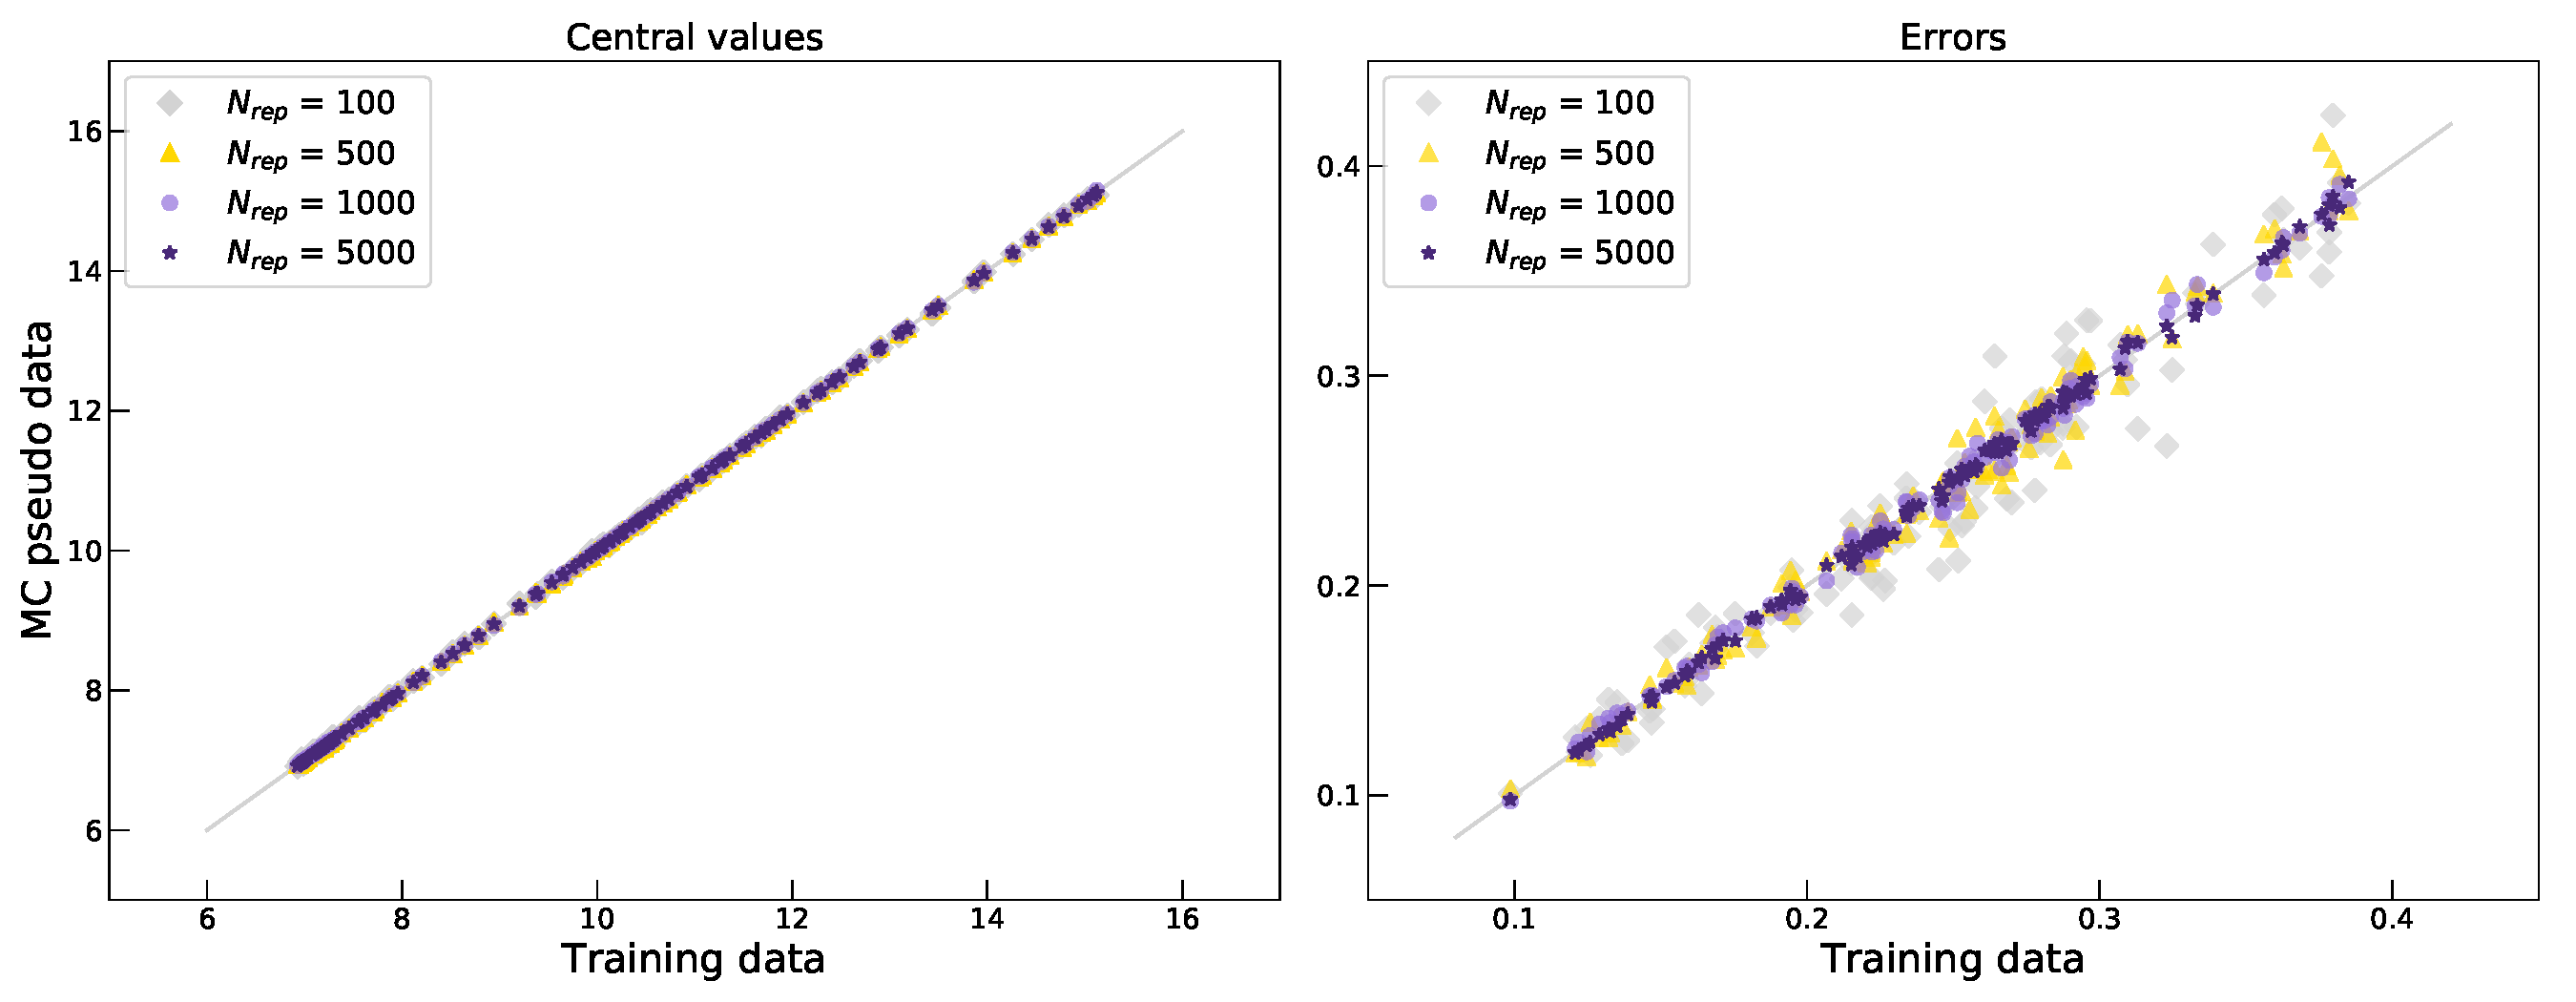
\includegraphics[width=0.99\textwidth]{plots/MC.pdf}
    \caption{Comparison between the original experimental central values
      $I_{\rm ZLP,i}^{\rm exp}$ (left panel) and the corresponding statistical
      uncertainties $\sigma_i^{(\rm stat)}$ with the results of averaging over
      a sample of $N_{\rm rep}$ Monte Carlo replicas generated by means of
      Eq.~(\ref{eq:MCreplicaGen}), for different values of
      $N_{\rm rep}$.
      }
    \label{fig:MC}
\end{figure}
%%%%%%%%%%%%%%%%%%%%%%%%%%%%%%%%%%%%%%%%%%%%%%%%5

To verify that this is the case,
Fig.~\ref{fig:MC} displays a comparison between the original experimental central values
$I_{{\rm ZLP},i}^{\rm (exp)}$ (left) and the corresponding 
total uncertainties $\sigma_i^{(\rm exp)}$ (right panel) with the results of averaging over
a sample of $N_{\rm rep}$ Monte Carlo replicas generated by means of
Eq.~(\ref{eq:MCreplicaGen}) for different number of replicas.
%
We find that $N_{\rm rep}=500$ is a value that ensures that both
the central values and uncertainties are reasonably well reproduced,
and we adopt it in what follows.


\subsection{Training strategy}
\label{sec:training}

The training of the neural-network model for the ZLP peak differs between
the cases of EEL spectra taken on vacuum,
where by construction $I_{\rm EEL}(\Delta E) =I_{\rm ZLP}^{\rm (mod)}(\Delta E)$,
and for spectra taken on samples. 
%
In fact, EEL spectra taken in the vacuum but close
to the sample might still receive inelastic contributions coming from the specimen.
%
When we talk about vacuum spectra, we consider exclusively those taken 
reasonably far from the surface of the analysed nanostructures.
%
In the latter case, we need to find a training strategy to make predictions
about the ZLP distribution in the low-loss regime, while we can not directly
train on data in this region.
%
As indicated by Eq.~(\ref{eq:ZLPseparation}), in order to avoid
biasing the results it is important to ensure that the model is trained only on the region of the spectra
where the ZLP dominates over the inelastic scatterings.
%
Then we can make predictions in the extrapolation regime based on these 
training parameters.
%
We now describe the training strategy that is adopted in both cases.

\paragraph{Training of vacuum spectra.}
%
For each of the $N_{\rm rep}$ generated Monte Carlo replicas, we train an independent
neural network as described in Sect.~\ref{sec:parametrisation}.
%
Fitting the neural networks parameters to the data is performed by minimisation of a
figure of merit (error function), defined as:
\begin{equation}
  \label{eq:chi2}
\begin{centering}
  E^{(k)}\lp \{\theta^{(k)}\}\rp = \frac{1}{n_{\rm dat}}\sum_{i=1}^{n_{dat}}\left(\frac{ I_{{\rm ZLP},i}^{{\rm (art)}(k)} -
  I_{{\rm ZLP},i}^{{\rm (mod)}}\lp \{\theta^{(k)}\}\rp }{\sigma_i^{(\rm exp)}}\right)^2, 
\end{centering}
\end{equation}

which is the $\chi^2$ per data point comparing each replicated ZLP intensity
with the corresponding model prediction.
%
In this expression $E^{(k)}\lp \{\theta^{(k)}\}\rp$ is the error for the values 
$\{\theta^{(k)}\}$ of the network weights and thresholds;
$I_{{\rm ZLP},i}^{{\rm (art)}(k)}$ is the $k$-th replica for the ZLP 
intensity and $I_{{\rm ZLP},i}^{{\rm (mod)}}$ is the model prediction on this
replica; and ${\sigma_i^{(\rm exp)}}$ again represents the error
associated to this experimental data point.\\

The chi-squared method is the cornerstone of almost all fitting, 
as it is an intuitively reasonable measure of how well the predictions fit the data. 
%
If the model predictions are all within one standard deviation from the data, 
then the $\chi^2$ per data point takes a value roughly equal to 1. 
%
In general, if $\chi^2/n_{dat}$ is of the order 1, we can say that the 
fit is a good approximation to the real data. 

In order to speed up the neural network training process, prior to the optimisation
all inputs and outputs are scaled to lie between $[0.1, 0.9]$ before
being feed to the network.
%
This preprocessing facilitates that
the neuron activation states will typically
lie close to the linear region of the sigmoid activation function.\\

The contribution to the figure of merit from the input experimental data, Eq.~(\ref{eq:chi2}),
needs in general to be complemented with that of theoretical constraints on the model.
%
For instance, when determining nuclear parton distributions~\cite{AbdulKhalek:2020yuc}, one needs to
extend Eq.~(\ref{eq:chi2}) with Lagrange multipliers to ensure that both the $A=1$ proton boundary
condition and the cross-section positivity are satisfied.
%
In the case at hand, our model for the ZLP should satisfy the constraint that $I_{\rm ZLP}(\Delta E)\to 0$
when $|\Delta E| \to \infty$, since far from $\Delta E\simeq 0$ the contribution from the ZLP
is completely negligible.
%
In order to implement this constraint, we add $n_{pd}$ pseudo-data points to the training dataset 
"far" away from the ZLP and we modify
the figure of merit Eq.~(\ref{eq:chi2}) accordingly,
\be
\label{eq:chi2modified}
E^{(k)}\lp \{\theta^{(k)}\}\rp \to E^{(k)}\lp \{\theta^{(k)}\}\rp +
\lambda \sum_{i'=1}^{n_{pd}}\left(
  I_{{\rm ZLP},i'}^{{\rm (mod)}}\lp \{\theta^{(k)}\}\rp \right)^2, 
  \ee
  where $\lambda$ is a Lagrange multiplier whose value is tuned to ensure that the $I_{\rm ZLP}(\Delta E)\to 0$
  condition
  is satisfied without affecting the description of the training dataset.
  %
  In other words, we add a contribution to the error function coming from these pseudo points in the
  higher-loss regime, making sure that the optimization of the error function also takes into account
  the fact that at higher losses the intensity should vanish.
  %
  However, when calculating the overall fit quality after training, we do not include the second term
  on the right-hand side of Eq.~(\ref{eq:chi2modified}) in the evaluation of the figure of merit, 
  as these "fake" datapoints do not give any physical
  information about the original dataset whatsoever.

  The pseudo-data points are added in the region $\lc \Delta E_{\rm pd}^{\rm (min)},
  \Delta E_{\rm pd}^{\rm (max)}\rc$, and symmetrically for negative energy losses.
  %
The value of $\Delta E_{\rm pd}^{\rm (min)}$
can be determined automatically by evaluating the ratio $\mathcal{R}_{\rm sig}$ between the central
experimental intensity and the total uncertainty in each data point,
\be
\label{eq:pdlocation}
\mathcal{R}_{\rm sig}(\Delta E_i)\equiv \frac{I_{{\rm ZLP}}^{(\rm exp)}(\Delta E_i)}{\sigma^{(\rm exp)}(\Delta E_i)} \, ,
\ee
which corresponds to the statistical significance for the $i$-th bin of $\Delta E$ to differ from the null hypothesis
(zero intensity) taking into account the experimental uncertainties.
%
For sufficiently large energy loss this ratio approaches 1, which indicates that we are essentially
fitting statistical noise. 
%
In order to avoid this and only fit data that is different from zero within errors, we determine the value
of $\Delta E_{\rm pd}^{\rm (min)}$ from the condition that $ \mathcal{R}_{\rm sig}(\Delta E_i) \simeq$ 1. 
%
We keep the training data in the region $\Delta E \le \Delta E_{\rm pd}^{\rm (min)}$ and the pseudo-data
points are added for $\lc \Delta E_{\rm pd}^{\rm (min)}, \Delta E_{\rm pd}^{\rm (max)}\rc$. 
%
The value of $\Delta E_{\rm pd}^{\rm (max)}$ can be chosen arbitrarily and can be as large as necessary
to ensure that $I_{\rm ZLP}(\Delta E)\to 0$ as $|\Delta E| \to \infty$.

We note that another important physical condition on the ZLP model, namely its positivity
(since in EEL spectra the intensity is just a measure of the number of counts in the
detector for a given value of the energy loss) is automatically satisfied since
we use a ReLU activation function for the last layer.
%
A further obvious requirement is that the best fit is independent of any assumptions 
made about the ZLP distribution. 
%
This requirement can be met by making sure the parametrisation is redundant: 
the size of the neural network used, and therefore the number of optimizable parameters, 
is much larger than the minimum required in order to reproduce the data. 
%
This redundancy can be verified {\it a posteriori}, that results are independent of 
the size and architecture of the neural network.\\

In this work we adopt the {\tt TensorFlow} neural-net libraries to assemble
the architecture illustrated in Fig.~\ref{fig:architecture}.
%
Before training, all weights and biases are initialized in a non-deterministic order
by the built-in global variable initializer. 
%
The optimisation of the figure of merit Eq.~(\ref{eq:chi2modified}) is carried
out by means of stochastic gradient descent (SGD) combined with backpropagation. The
specific SGD optimizer used is the Adam algorithm.
%
The hyper-parameters of the optimisation algorithm such as the learning rate
have been adjusted to ensure proper learning is reached in the shortest amount
of time possible.
%
Given that we have a extremely flexible parametrisation, one should be careful
to avoid overlearning the input data.
%
Here over-fitting is avoided by means of a cross-validation stopping criterion.
%
We separate the input data into training a validation subsets, with a 80\%/20\% splitting
which partition varies randomly for each Monte Carlo replica.
%
We then run the optimiser for a very large number of iterations and store both
the state of the network and the value
of the figure of merit Eq.~(\ref{eq:chi2}) restricted to the validation
dataset, $E^{(k)}_{\rm val}$ (which is not used for the training).
%
We are not looking for the absolute minimum of the error function, 
but we rather search for an optimal stopping point to avoid overfitting. 
%
At this optimal stopping point, it reproduces the information contained in the dataset, 
but not its statistical fluctuations.
%
This point can be determined by the formulation of a stopping criterion, 
making it possible to, once the network completed the training, 
choose the parametrization of the network weights right before it 
entered the overlearning regime. 
%
The optimal stopping point is determined  for each replica
by keeping track of the figure of merit, which typically evolutes
as depicted in Fig.~\ref{fig:costs}. 
%
The specific network configuration that leads to the deepest minimum of $E^{(k)}_{\rm val}$:
is chosen {\it a posteriori}, that's why it is called look-back stopping, 
a method that has been widely used in the context
of neural networks.
%
The number of epochs should be chosen high enough to reach for each replica 
the absolute minimum of $E^{(k)}_{\rm val}$, 
rather than a local minimum.
For this work we need approximately 40,000 epochs to guarantee overlearning.
%
This corresponds to a serial running time of 60 seconds per replica when running the optimization on a 
single CPU for a set of 500 datapoints.
%
Once the training of all the $N_{\rm rep}$ neural network models for the ZLP has been carried
out as specified above, we quantify the overal fit quality of the model by computing the
$\chi^2$ defined as
\begin{equation}
  \label{eq:chi2_final}
\begin{centering}
  \chi^2 = \frac{1}{n_{\rm dat}}\sum_{i=1}^{n_{dat}}\left(\frac{ I_{{\rm ZLP},i}^{{\rm (exp)}} -
 \la I_{{\rm ZLP},i}^{{\rm (mod)}}\ra_{\rm rep} }{\sigma_i^{(\rm exp)}}\right)^2, 
\end{centering}
\end{equation}
which is the analog of Eq.~(\ref{eq:chi2_final}) now comparing the average model prediction
to the original experimental data values.
%
A value $\chi^2 \simeq 1$ indicates that a satisfactory description of the experimental data,
within the corresponding uncertainties, has been achieved.
%
Note that in realistic scenarios $\chi^2$ can deviate from unity, for instance when
some source of correlation between the experimental uncertainties has been neglected
or when the errors on the data points have been over- or underestimated.


\paragraph{Training of sample spectra.}

The training strategy in the case of EEL spectra taken on samples (rather than on vacuum) must be adjusted
to account for the fact that the input data set, Eq.~(\ref{eq:IeelTot}), receives contributions
both from the ZLP and from inelastic scatterings.
%
To avoid biasing the ZLP model, we should make sure to include only the former contributions 
in the training dataset.
%
Else, if we were to train the neural network on data that contains also inelastic contributions,
subsequent subtraction to the EEL spectra would make us lose important information.

We can illustrate the situation at hand with the help of a toy model for the low-loss
region of EEL spectra, represented in
Fig.~\ref{fig:EELS_toy}.
%
Let us use a general assumption that the ZLP is described by a 
Gaussian distribution with a standard deviation of $\sigma_{\rm ZLP}=0.3$ eV,
and that the contribution from the
inelastic interactions with the sample can be approximated in the low-loss
regime by $I_{\rm inel}(\Delta E)\propto \lp \Delta E - E_{\rm bg}\rp^b$ with $E_{\rm bg}=1.5$
and $b=0.5$. 
%
The motivation for this
choice will be explained in Sect.~\ref{sec:results_sample}.
%
We display the separate contributions from $I_{\rm ZLP}$
and $I_{\rm inel}$, as well as the total intensity,  
with the inset showing the values of the corresponding derivatives, $dI/d\Delta E$.

%%%%%%%%%%%%%%%%%%%%%%%%%%%%%%%%%%%%%%%%%%%%%
\begin{figure}[t]
    \centering
    \includegraphics[width=0.7\textwidth]{plots/Toy.pdf}
    \caption{A toy model for a generic EEL spectrum and its
      derivatives (in the inset).
      %
      We show the separate contributions from $I_{\rm ZLP}$
      and $I_{\rm inel}$ as well as their sum.
      %
      We indicate the two regions used for the model training ($I$ and $III$),
      while the trained model is interpolated to region $II$, 
      defined for $\Delta E_I \le \Delta E \le \Delta E_{II}$.}
    \label{fig:EELS_toy}
\end{figure}
%%%%%%%%%%%%%%%%%%%%%%%%%%%%%%%%%%%%%%%%%%%%%%%%%

The toy model of Fig.~\ref{fig:EELS_toy} is sufficiently general to draw
a number of useful considerations concerning the relation between $I_{\rm ZLP}$ and $I_{\rm inel}$
in realistic spectra:

\begin{itemize}

\item The ZLP intensity, $I_{\rm ZLP}(\Delta E)$, is a monotonically decreasing function
  and thus its derivative is always negative.

\item  The first local minimum of the total spectrum, $dI_{\rm EELS}/d\Delta E|_{\Delta E_{\rm min}}=0$, corresponds
  to a value of $\Delta E$ for which the contribution from the inelastic emissions is already
  significant.

\item The value of $\Delta E$ for which $I_{\rm inel}$ starts to contribute to the total spectrum
  corresponds to the position where the intensity derivatives in-sample and in-vacuum  start to differ.
  %
  We note that a direct comparison between the overal magnitude of the sample and vacuum ZLP
  spectra is in general not possible, as explained in Sect.~\ref{sec:eels}. 
\end{itemize}

These considerations suggest that when training the ML model on EEL spectra taken on samples,
the following categorisation should de adopted:

\begin{enumerate}

\item For small energy losses such that $\Delta E \le \Delta E_I$ (region $I$),
  the model training  proceeds in the same way as for the vacuum case
  via the minimisation of Eq.~(\ref{eq:chi2}).

\item  
  For $\Delta E \ge \Delta E_{II}$ (region $III$), we use instead Eq.~(\ref{eq:chi2modified})
  without the contribution from the input data, since for such values
  of $\Delta E$ one has that $I_{\rm inel}\gg I_{\rm ZLP}$.
  %
  In other words, we only fit on the pseudo data and therefore
  the only information that the region $III$ provides
  on the model is the one arising from the implementation
  of the constraint that $I_{\rm ZLP}(\Delta E\to \infty)\to 0$.

\item The EELS data in region $II$, defined by $\Delta E_I \le \Delta E \le \Delta E_{II}$,
  is excluded from the training dataset, given that in this region the contribution to $I_{\rm EEL}$
  coming from $I_{\rm inel}$ is already significant.
  %
  The model predictions in this regime are obtained from an interpolation
  of the predictions obtained in regions $I$ and $III$.

\end{enumerate}

This classification introduces two new hyper-parameters of our model, $\Delta E_I$ and
$\Delta E_{II}$, that need to be specified before the training.
%
They should satisfy $\Delta E_I \le \Delta E_{\rm min}$ and $\Delta E_{II} \ge \Delta E_{\rm min}$,
with $\Delta E_{\rm min}$ being the position of the first local minimum of $I_{\rm EEL}$.
%
Let's interpret this physically: $\Delta E_{\rm min}$ is the first local minimum, which means that 
the inelastic contributions are significantly present.
%
Training the data for higher than this value, we are sure that our training data includes
at least some amount of inelastic scatterings.
%
Therefore, it is certain that we need to cut the training data already at a lower energy loss,
so $\Delta E_I \le \Delta E_{\rm min}$.
%
As indicated by the toy spectra of Fig.~\ref{fig:EELS_toy}, a suitable value for $\Delta E_{I}$
would be somewhat above the onset of the inelastic contributions: this way we maximise
the amount of training data while ensuring that $I_{\rm EEL}$ is still dominated
by $I_{\rm ZLP}$.

We can use the derivatives of the spectra, $dI_{\rm EEL}/d\Delta E$, to select suitable minimum and
maximum values for $\Delta E_I$. 
%
Using first and second derivatives is an often-used feature extraction method to achieve a relatively 
high accuracy with a low computational complexity. 
%
In an ideal microscope the electron beam would be perfectly monochromatic, 
correspondingly the ZLP would appear as a delta function in an EEL spectrum \cite{Rafferty:2000}. 
%
In practice the ZLP has a finite width defining the energy resolution of the system. 
%
Concerning $\Delta E_I $, its minimum possible value is selected as the value where the derivate taken on the sample
data start to different significantly as compared to those spectra taken on vacuum.
%
This value is obtained by looking at the ratio of the derivatives of the spectra compared to the vacuum derivatives:
\be
R_{dI/d \Delta E} =  \left( \frac{dI_{\rm ZLP}/d\Delta E}{dI_{\rm EEL}/d\Delta E}\right). 
\ee
%
For low energy losses this ratio equals 1, which means that in the low-loss regime
the spectra recorded in vacuum and on specimens behave similar.
%
However, at some energy loss $\Delta E_{I,min}$ the
sample spectrum stops monotonically decreasing and the ratio deviates from 1. 
%
It is this point where the contributions from the sample start to change the shape of
the ZLP distribution and we can use this measure to mark the transition from 
regime I to regime II in Fig.~\ref{fig:EELS_toy}.
%
We know that the hyper-parameter $\Delta E_I$ should satisfy 
$\Delta E_{I,min} \le \Delta E_I \le \Delta E_{\rm min}$,
which corresponds to the region where $R_{dI/d \Delta E} \ne  1$ and $R_{dI/d \Delta E} \ge 0$.
%
The neural network will be trained on a range of different $\Delta E_I$ values within this interval,
and the optimal choice will be determined {\it a posteriori} from the results.
%
Also, generating results for different values of $\Delta E_I$ makes us able to 
cross-validate on the stability of our results regardless of the exact choice of this
hyperparameter.

Another important difference as compared to the training of the vacuum spectra is that each of the sample
spectra will have different values of $\Delta E_{\rm min}$ and thus of $\Delta E_I$. 
%
For this reason we calculate $\Delta E_{\rm min}$  for each of the sample spectra and we use the highest of these
as the maximum value for the hyper-parameter $\Delta E_I$. 
%
As we determine the best choice of $\Delta E_I$ after training for each of the spectra separately, 
we are sure to capture all suitable results and select the best value for each individual spectrum. \\

Concerning $\Delta E_{II}$, its minimum value should mark the region where $I_{\rm ZLP}(\Delta E\to \infty)\to 0$. 
%
It is the value where we start adding pseudo-data, so $\Delta E_{II}$ = $\Delta E_{\rm pd,min}$.
%
In order to implement this constraint, similar to the previous section (Eq.~(\ref{{eq:pdlocation}}))
we look at the ratio 
$\mathcal{R}_{\rm sig}(\Delta E_i)$ to determine the energy loss $\Delta E_{\rm pd}$ at 
which the contributions from the vacuum-recorded ZLP vanish. 
%
As a measure, we use the energy loss value where the ratio $\mathcal{R}_{\rm sig}(\Delta E_i)$ drops below 1,
as in this regime we would be fitting statistical noise.
%
We set the value of $\Delta E_{II}$ equal to this energy loss and add pseudo-data points for $\Delta E \ge \Delta E_{II}$.
%
Note that in this region the intensity of the ZLP is several orders of magnitude smaller than the intensity 
of the elastic emissions and therefore the exact choice of $\Delta E_{II}$ does not listen too closely.

Now that we have parametrised the 


% Discussion of results in vacuum
% including closure test validation
\section{ZLP parametrisation for vacuum spectra}
\label{sec:results_vacuum}

Now we move to present the application of the strategy presented in the previous
section to the parametrisation of ZLP spectra acquired in vacuum.
%
Applying our model to this case has a two-fold motivation.
%
First of all, we aim to demonstrate that our model is flexible enough to effectively reproduce the
input EELS measurements for a range of variations of the operation parameters of the microscope.
%
Second, it will allow us to provide a calibration prediction
useful for the case of the in-sample measurements.
%
Such calibration is necessary since, as explained in Sect.~\ref{sec:training}, some of the model
hyper-parameters are determined by the comparison of the intensity derivatives
between spectra taken in vacuum and those in sample.

In this section, first of all we present the input dataset and motivate the choice
of training settings and model hyperparameters.
%
Then we validate the model training by assessing the fit quality.
%
Lastly, we study the dependence of the model predictions in its various input
variables, and study the dependence of the model uncertainties upon
the removal of a subset of the training dataset.

\subsection{Training settings}

In Table~\ref{table:vacuumdata} we collect the main properties of the EELS spectra acquired in vacuum to train the neural
    network model.  For each set of spectra, we indicate the exposure time $t_{\rm exp}$, the beam energy
    $E_b$, the number of spectra $N_{\rm sp}$ recorded for these operation conditions, the number $N_{\rm dat}$ of
    bins in each spectrum, the range in electron energy loss $\Delta E$,
    and the average full width at half maximum (FWHM)
    evaluated over the $N_{\rm sp}$ spectra with the corresponding variance.
    %
    All the spectra  listed on Table~\ref{table:vacuumdata}
    were acquired with a Titan TEM equipped with a Schottky field emitter.
    %
    We point out that since here
    we are interested in the low-loss region, $\Delta E_{\rm max}$ does not need
    to be too large, and in any case the large $\Delta E$ behaviour of the model is fixed
    by the constraint implemented by Eq.~(\ref{eq:chi2modified}).

%%%%%%%%%%%%%%%%%%%%%%%%%%%%%%%%%%%%%%%%%%%%%%%%%%%%%%%%%%%%%%%%%%%%%%%%%%%%%%%%%%%%%%%%%%%%%
%%%%%%%%%%%%%%%%%%%%%%%%%%%%%%%%%%%%%%%%%%%%%%%%%%%%%%%%%%%%%%%%%%%%%%%%%%%%%%%%%%%%%%%%%%%%%
\begin{table}[t]
  \begin{center}
            \renewcommand{\arraystretch}{1.50}
  \begin{tabular}{@{}ccccccccc}
\br
Set & $t_{\rm exp}$ {(}ms{)} & $E_{\rm b}$ {(}keV{)} & $N_{\rm sp}$ & $N_{\rm dat}$ & $\Delta E_{\rm min}$~(eV)  & $\Delta E_{\rm max}$~(eV)  & FWHM~(meV)  \\ 
\mr
1        & 100                 & 200                  & 15          & 2048               & -0.96              & 8.51     & $47\pm7 $         \\
2        & 100                 & 60                   & 7           & 2048               & -0.54              & 5.59    & 
$ 50 \pm 4$         \\
3        & 10                  & 200                  & 6          & 2048               & -0.75              & 5.18      & 
$ 26 \pm 3$         \\
4        & 10                  & 60                   & 6           & 2048               & -0.40              & 4.78       & 
$ 34\pm 2$         \\ 
\br
  \end{tabular}
    \end{center}
  \caption{\small Summary of the main properties of the EELS spectra acquired in vacuum to train the neural
    network model.  For each set of spectra, we indicate the exposure time $t_{\rm exp}$, the beam energy
    $E_b$, the number of spectra $N_{\rm sp}$ recorded for these operation conditions, the number $N_{\rm dat}$ of
    bins in each spectrum, the range in electron energy loss $\Delta E$,
    and the average FWHM evaluated over the $N_{\rm sp}$ spectra with the corresponding standard deviation
  }
   \label{table:vacuumdata}
\end{table}
%%%%%%%%%%%%%%%%%%%%%%%%%%%%%%%%%%%%%%%%%%%%%%%%%%%%%%%%%%%%%%%%%%%%%%%%%%%%%%%%%%%%%%%%%%%%%%%%%5
%%%%%%%%%%%%%%%%%%%%%%%%%%%%%%%%%%%%%%%%%%%%%%%%%%%%%%%%%%%%%%%%%%%%%%%%%%%%%%%%%%%%%%%%%%%%%

    The energy resolution of these spectra, quantified by the value of their FWHM, ranges
    from 26 meV to 50 meV depending on the specific operation conditions of the microscope,
    with an standard deviation between 2 and 7 meV.
    %
    The value of the FWHM varies only mildly with the value of the beam energy $E_b$
    but grows by around a factor two for spectra collected at larger exposure times $t_{\rm exp}$.
    %
    A total of almost $7\times 10^4$ independent measurements will be thus used for the ZLP model
    training on the vacuum spectra.
    %
    As will be highlighted in Sects.~\ref{eq:depdeltae} and~\ref{eq:depebeam}, one of the advantages of our ZLP model is that it can extrapolate its predictions
    to other operation conditions beyond those used for the training.

Following the strategy presented in Sect.~\ref{sec:methodology}, first of all we combine the $N_{\rm sp}$ spectra
corresponding to each of the four sets of operation conditions and determine the statistical uncertainty
associated to each energy loss bin by means of Eq.~(\ref{eq:sigmaiexp}).
%
For each of the training sets, we need to determine the value of $\Delta E_{\rm pd}^{\rm (min)}$
that defines the range for which we add the  pseudo-data
that imposes the correct $\Delta E \to \infty$ limit of the model.
%
This value is determined
by inspecting the ratio between the central experimental value of the total
EELS intensity, $I_{{\rm EEL},i}^{(\rm exp)}$, and its corresponding
total uncertainty defined in Eq.~(\ref{eq:sigmaiexp}).


      
%%%%%%%%%%%%%%%%%%%%%%%%%%%%%%%%%%%%%%%%%%%%%%%%%%%%%%%%%%%%%%%%%%%%%%%%%%%%%%%%%%%%%%%%%%%%%%%%%%%%%%%%%%%%
\begin{figure}[t]
    \centering
    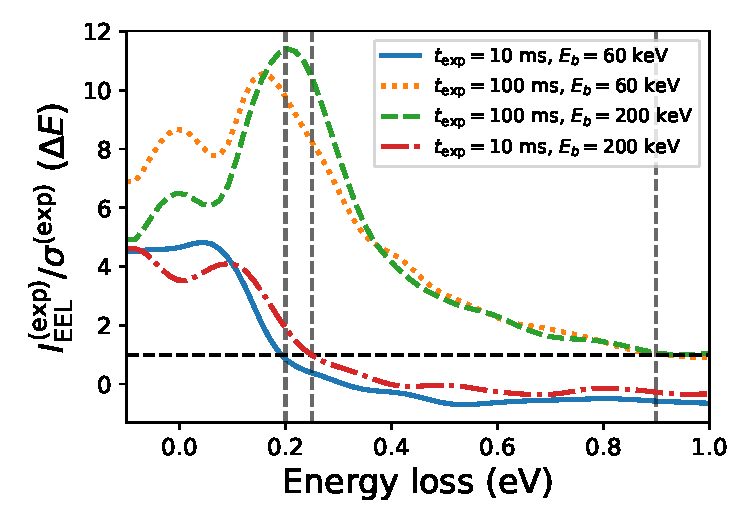
\includegraphics[width=120mm]{plots/intensity_to_error_ratio.pdf}
    \caption{\small The ratio between the central experimental value of the total
      EELS intensity, $I_{{\rm EEL},i}^{(\rm exp)}$, and the corresponding
      total uncertainty defined in Eq.~(\ref{eq:sigmaiexp}).
      %
      Results are shown for the four combinations of $t_{\rm exp}$
      and $E_{b}$ listed in Table~\ref{table:vacuumdata}.
      %
      The vertical dashed lines mark the values of $\Delta E$ for which
      this ratio becomes smaller than unity, which indicates when the input
      data starts to be dominated by the statistical noise.
      }
    \label{fig:intensityratio}
\end{figure}
%%%%%%%%%%%%%%%%%%%%%%%%%%%%%%%%%%%%%%%%%%%%%%%%%%%%%%%%%%%%%%%%%%%%%%%%%%%%%%%%%%%%%%%%%%%%%%%%%%%%%%%%%%%%%%%%%

Fig.~\ref{fig:intensityratio} displays this ratio
for the four combinations of $t_{\rm exp}$
and $E_{b}$ listed in Table~\ref{table:vacuumdata}.
%
The vertical dashed lines indicate the values of $\Delta E$ for which
this ratio becomes smaller than unity.
%
For larger $\Delta E$, the EELS spectra become
consistent with zero within uncertainties and can thus be discarded and replaced
by the pseudo-data constraints.
%
Thus the cross-over value of $\Delta E$  where the ratio satisfies $I/\sigma\simeq 1$
is a reasonable choice for $\Delta E_{\rm pd}^{\rm (min)}$
%
The total uncertainty of the pseudo-data points is chosen to be
\be
\sigma_j^{(\rm pd)} = \frac{1}{10}I_{{\rm EEL}}^{\rm (exp)}\lp \Delta E = \Delta E_{\rm pd}^{\rm (min)}\rp \,, \quad 
j= 1,\ldots,N_{\rm pd} \, .
\ee
The factor of 1/10 is found to be suitable to ensure that the constraint
is enforced without distorting
the training to the experimental data.
%
We note from Fig.~\ref{fig:intensityratio} that $\Delta E_{\rm pd}^{\rm (min)}$ will
depend on general on the operation conditions.
%
We find that
for our training samples $\Delta E_{\rm pd}^{\rm (min)} \simeq 200$ meV for $t_{\rm exp}=10$ ms
and $\simeq  900$ meV for 100 ms, roughly independent on the value of $E_b$.

The input experimental measurements listed in Table~\ref{table:vacuumdata} are used
to to generate a sample of $N_{\rm rep}=500$ Monte Carlo replicas
and train an individual neural network model to each of these replicas.
%
The end result of the procedure is a set of model replicas,
\be
\label{eq:modelreplicas}
I_{\rm ZLP}^{\rm (mod)(k)}(\Delta E, E_{b},t_{\rm exp}) \, , \quad k=1,\ldots,N_{\rm rep} \, ,
\ee
which can be used to provide a prediction for the intensity of the ZLP
for arbitrary values of $\Delta E$,  $E_{b}$, and $t_{\rm exp}$.
%
Eq~(\ref{eq:modelreplicas})
provides the sought-for representation of the probability density in the space of ZLP models.
%
For this sample of replicas one can evaluate
statistical estimators such as averages, variances, and correlations (as well
as higher moments) by means of
the usual expressions, for instance
\be
\label{eq:average}
\la I_{\rm ZLP}^{\rm (mod)}( \{z_1\}) \ra = \frac{1}{N_{\rm rep}}\sum_{k=1}^{N_{\rm rep}}
I_{\rm ZLP}^{\rm (mod)(k)}( \{z_1\}) \, ,
\ee
\be
\label{eq:standarddev}
\sigma_{I_{\rm ZLP}}^{\rm (mod)}( \{z_1\})  = \lp \frac{1}{N_{\rm rep}-1} \sum_{k=1}^{N_{\rm rep}}
\lp  I_{\rm ZLP}^{\rm (mod)(k)}  - \la I_{\rm ZLP}^{\rm (mod)}  \ra   \rp \rp^{1/2} \, ,
\ee
\be
\rho \lp \{z_1\},\{z_2\}\rp = \frac{ \la I_{\rm ZLP}^{\rm (mod)}( \{z_1\} ) I_{\rm ZLP}^{\rm (mod)}( \{z_2\} ) \ra
- \la I_{\rm ZLP}^{\rm (mod)}( \{z_1\} )\ra \la I_{\rm ZLP}^{\rm (mod)}( \{z_2\} ) \ra}{\sigma_{I_{\rm ZLP}}^{\rm (mod)}( \{z_1\} )\sigma_{I_{\rm ZLP}}^{\rm (mod)}( \{z_2\} )}
\ee
where as in the previous section $\{z_l\}$ denotes a possible set of input variables for the model.
We now discuss some of features of this ZLP vacuum model, here $\{z_l\}=\lp \Delta E, E_{b},t_{\rm exp}\rp$.

\subsection{Fit quality}
%
To begin with, we would like to quantify the overall fit quality of the model and demonstrate that it is flexible enough
to describe all the available input datasets.
%
In Table~\ref{table:chi2summary} we indicate the values of the final $\chi^2$ per data point,
    Eq.~(\ref{eq:chi2_final}), as well as the average values of the error Eq.~(\ref{eq:chi2})
    over the training and validation subsets, for each of the four sets of spectra listed in
    Table~\ref{table:vacuumdata} as well as for the total dataset.
    %
    We recall that for a satisfactory training one expects $\chi^2 \simeq 1$
    and $\la E_{\rm tr}\ra \simeq \la E_{\rm val}\ra \simeq 2 $~\cite{Forte:2002fg}.
    %
    From the results of this table we can see that these expectations are satisfied,
    both for the individual sets and for the total dataset.

    Then Fig.~\ref{fig:chi2_distributions} displays  the $\chi^2$  distributions
    evaluated for the training and validation sets
      of the $N_{\rm rep}=500$ replicas of the sample trained on the spectra
      listed in Table~\ref{table:vacuumdata}.
      %
      Note that the training/validation partition differs at random for each replica.
      %
      The $\chi^2_{\rm tr}$ distribution peaks at $\simeq .7$, indicating that a satisfactory model training
      has been achieved, however that the errors on our data points have been slightly overestimated.
      %
      We emphasize that the stopping criterion for the neural net training adopted here never considers
      the numerical values of the error function and determines proper learning entirely from
      the global minima of $E_{\rm val}^{(k)}$.
      %
      From Fig.~\ref{fig:chi2_distributions} we also observed that  $\chi^2_{\rm tr}$ distribution peaks at
      a slighter higher value, $\simeq 1$, and is broader that its corresponding training counterpart.
      %
      These results confirm both that a satisfactory model training that prevents overlearning
      has been achieved as well as an appropriate estimate of the statistical uncertainties
      affecting the original EEL spectra.
    
%%%%%%%%%%%%%%%%%%%%%%%%%%%%%%%%%%%%%%%%%%%%%%%%%%%%%%%%%%%%%%%%%%%%%%%%%%%%%%%%%%%%%%%%%%%%%%%%%%%%%%%%%%%%
\begin{figure}[t]
    \centering
    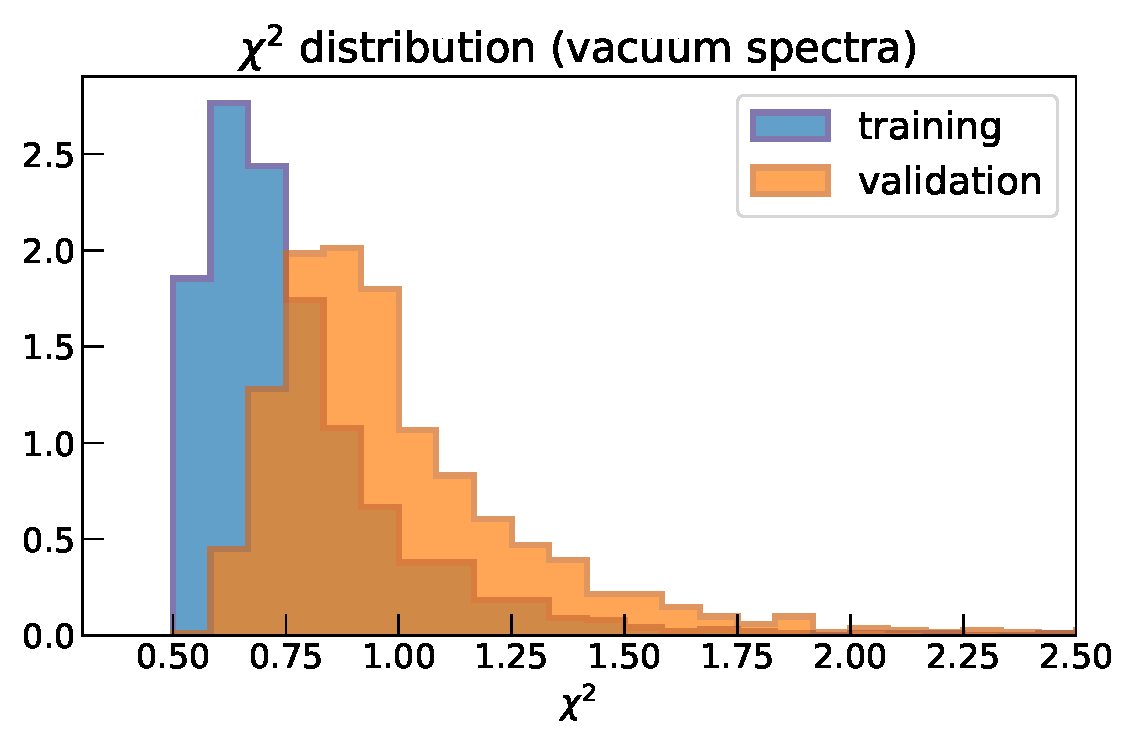
\includegraphics[width=0.49\textwidth]{plots/chi2_distributions.pdf}
    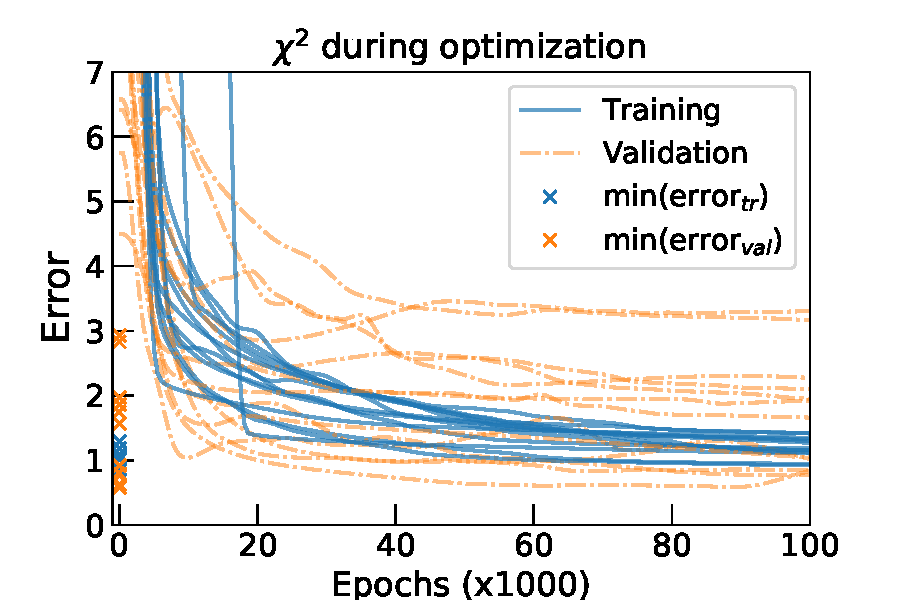
\includegraphics[width=0.49\textwidth]{plots/train_val_error_271.pdf}
    \caption{Left: The $\chi^2$ (per data point) distribution evaluated for the training and validation sets
      of the $N_{\rm rep}=500$ replicas of the sample trained on the spectra
      listed in Table~\ref{table:vacuumdata}. Right: the progress of the training and validation error over
      the course of the optimization. Number of replicas is taken small for clarity.
      The final $\chi^2$ is marked on the y-axis and shows how the distribution of training errors
      is more narrow and centered at a lower value compared to the validation errors. }
    \label{fig:chi2_distributions}
\end{figure}
%%%%%%%%%%%%%%%%%%%%%%%%%%%%%%%%%%%%%%%%%%%%%%%%%%%%%%%%%%%%%%%%%%%%%%%%%%%%%%%%%%%%%%%%%%%%%%%%%%%%%%%%%%%%%%%%%%%
%%%%%%%%%%%%%%%%%%

\begin{table}[h]
  \begin{center}
            \renewcommand{\arraystretch}{1.35}
  \begin{tabular}{@{}cccc}
\br
Set & $\chi^2$  &  $\la E_{\rm tr}\ra$   &  $\la E_{\rm val}\ra$ \\
\mr
1        &           0.998        &      1.702            &  1.970  \\
2        &           0.733        &     1.408            &  1.767  \\
3        &           0.697        &    1.391            &  1.800  \\
4        &           0.593        &    1.201            &  1.761  \\
\mr
Total    &           0.771        &    1.470            &  1.853  \\
\br
  \end{tabular}
    \end{center}
  \caption{\small \small The values of the final $\chi^2$ per data point,
    Eq.~(\ref{eq:chi2_final}), as well as the average values of the error Eq.~(\ref{eq:chi2})
    over the training and validation subsets, for each of the four sets of spectra listed in
    Table~\ref{table:vacuumdata} as well as for the total dataset.
  }
   \label{table:chi2summary}
\end{table}
%%%%%%%%%%%%%%%%%%%%%%%%%%%%%%%%%%%%%%%%%%%%%%%%%%%%%%%%%%%%%%%%%%%%%%%%%%%%%%%%%%%%%%%%%%%%%%%%%5
%%%%%%%%%%%%%%%%%%%%%%%%%%%%%%%%%%%%%%%%%%%%%%%%%%%%%%%%%%%%%%%%%%%%%%%%%%%%%%%%%%%%%%%%%%%%%

\subsection{Dependence on the electron energy loss}
\label{eq:depdeltae}

Having demonstrated that our neural network model provides a satisfactory description
of all the input EEL spectra, we now present its  predictions for specific
choices of the input parameters.
%
First of all, we investigate the dependence of the results as a function of the
electron energy loss $\Delta E$.
%
Fig.~\ref{fig:EELS_vacuum_DeltaE} displays the central value and 68\% confidence level uncertainty band
for the ZLP model as a function
of electron energy loss $\Delta E$
evaluated using Eqns.~(\ref{eq:average}) and~(\ref{eq:standarddev}).
%
We display results corresponding to 
three different values of $E_b$  and for both
$t_{\rm exp}=10$ ms (left)  and $t_{\rm exp}=100$ ms (right panel).
%
We emphasize that no training data with $E_b=120$ keV has been used and thus our prediction
in that case arises purely from the model interpolation.
%
It is interesting to note how both the overall normalisation and the shape of
the predicted ZLP depend on the specific operation conditions.

%%%%%%%%%%%%%%%%%%%%%%%%%%%%%%%%%%%%%%%%%%%%%%%%%%%%%%%%%%%%%%%%%%%%%%%%%%%%%%%%%%%%%%%%%%%%%%%%%%%%%%%%%%%%
\begin{figure}[t]
    \centering
    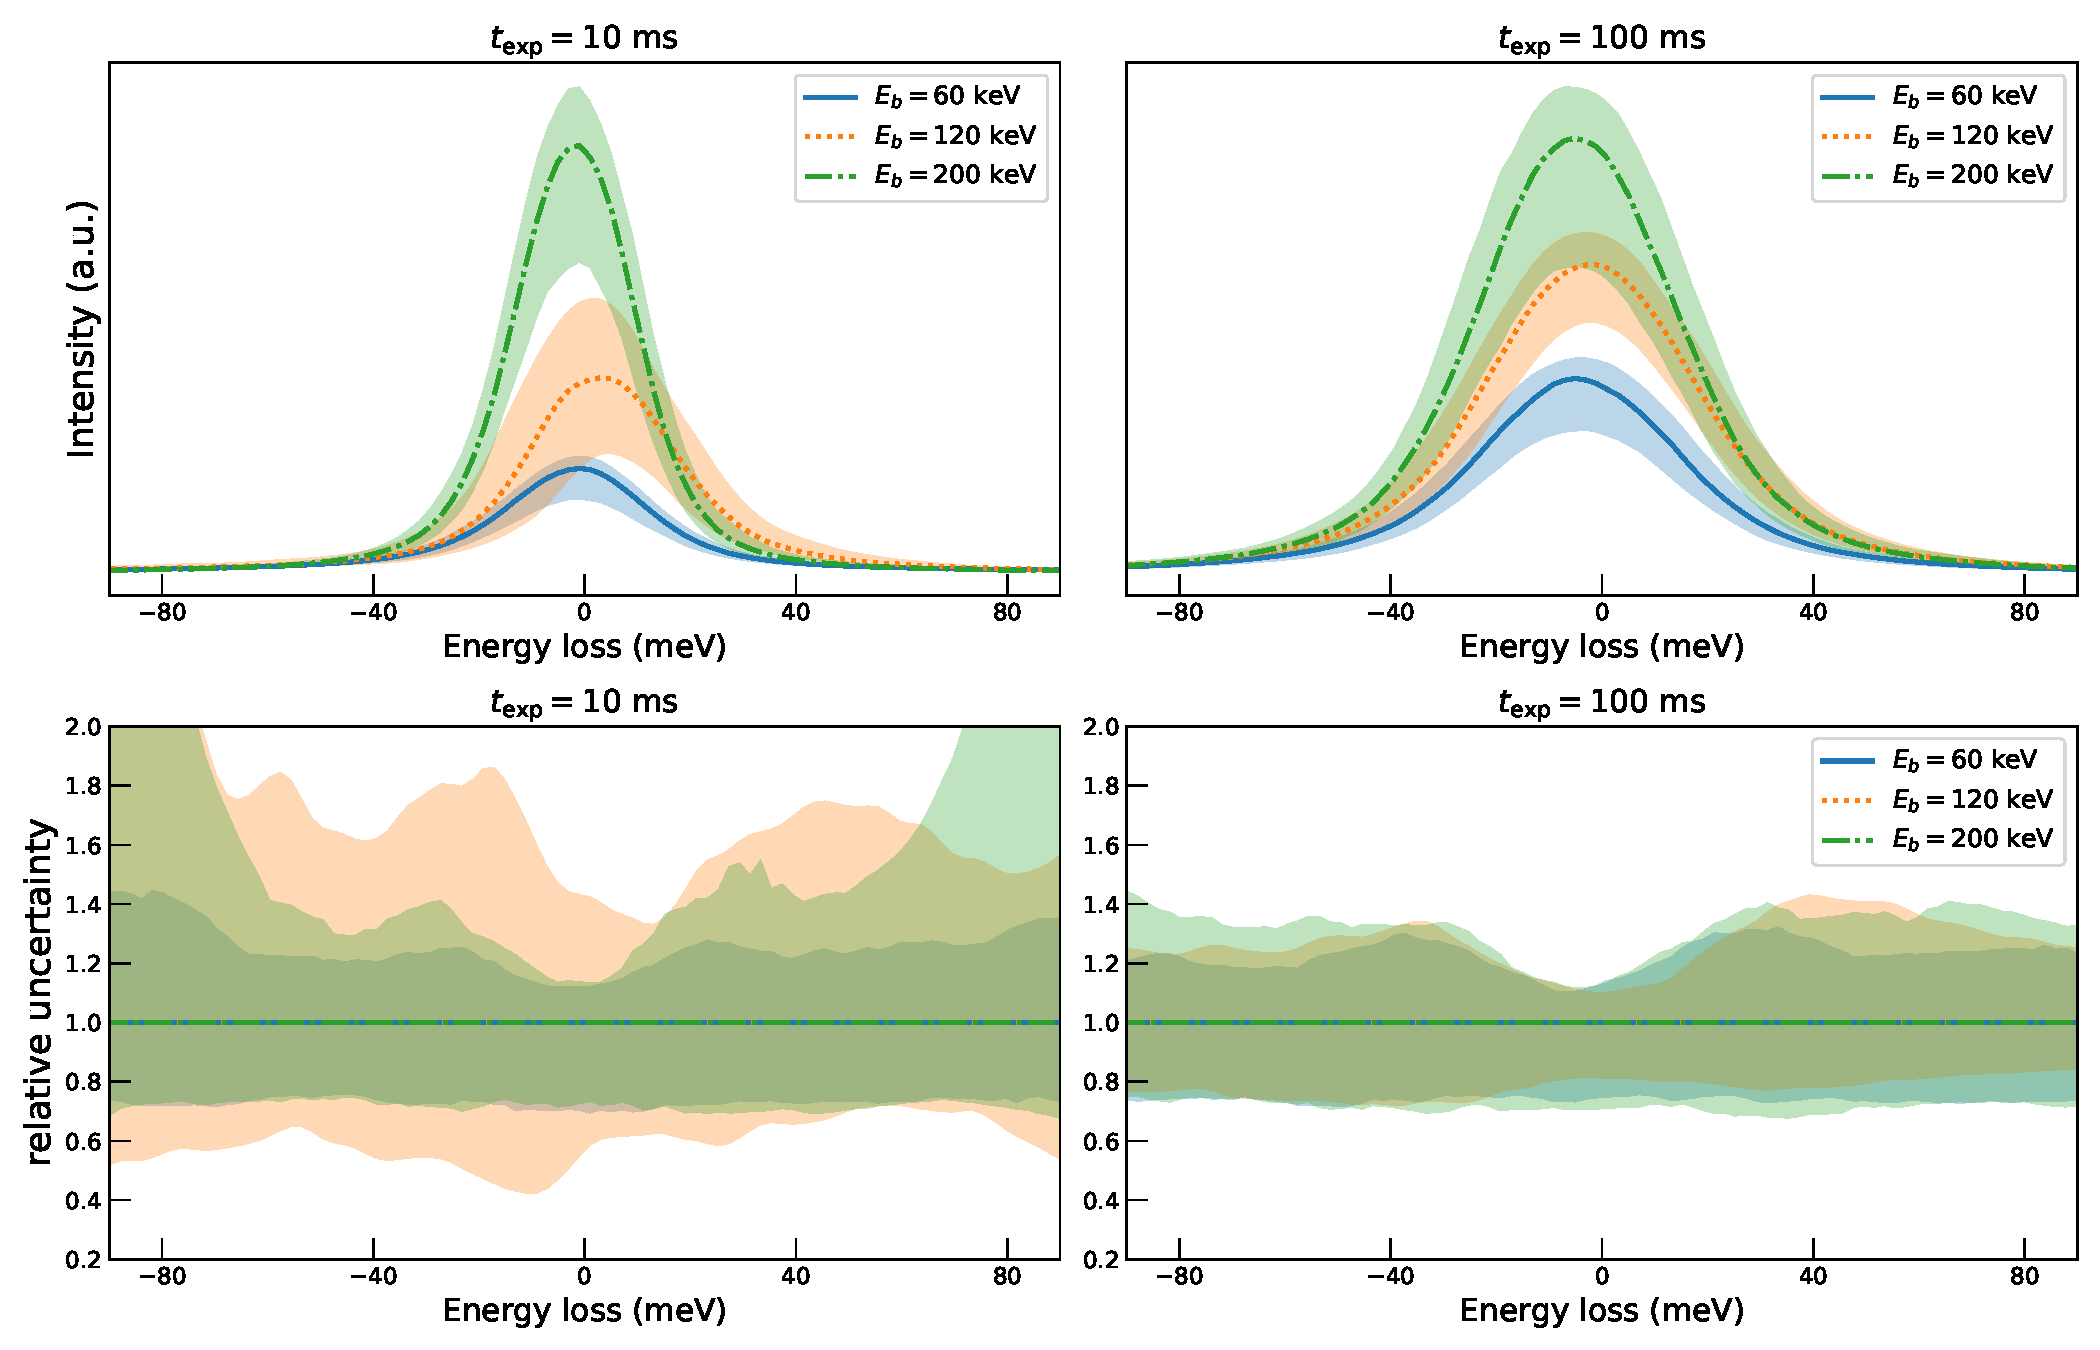
\includegraphics[width=170mm]{plots/deltaE_dependence_vacuum.pdf}
    \caption{\small Top: the central value and 68\% confidence level uncertainty band
      for the ZLP model as a function
      of electron energy loss $\Delta E$
      evaluated using Eqns.~(\ref{eq:average}) and~(\ref{eq:standarddev}).
      %
      We display results corresponding to 
      three different values of $E_b$  and for both
      $t_{\rm exp}=10$ ms (left)  and $t_{\rm exp}=100$ ms (right panel).
      %
      Note that no training data with $E_b=120$ keV has been used and thus our prediction
      in that case arises purely from the model interpolation.
      %
      Bottom: the corresponding relative uncertainty as a function of $\Delta E$
      for each of the three values of $E_b$.
      \label{fig:EELS_vacuum_DeltaE}}
\end{figure}
%%%%%%%%%%%%%%%%%%%%%%%%%%%%%%%%%%%%%%%%%%%%%%%%%%%%%%%%%%%%%%%%%%%%%%%%%%%%%%%%%%%%%%%%%%%%%%%%%%%%%%%%%%%%%%%%%%%

In the bottom panel of Fig.~\ref{fig:EELS_vacuum_DeltaE} we show
the corresponding relative uncertainty as a function of $\Delta E$
for each of the three values of $E_b$.
%
Recall that in this work we allow for non-Gaussian distributions and thus the central
value is the mean of the distribution while the error band in general will
be asymmetric.
%
In the case of the $t_{\rm exp}=10$ ms results, we see how the model prediction
at $E_b=120$ keV typically exhibits larger uncertainties than the predictions
for the two values of $E_b$ for which we have training data.
%
In the case of $t_{\rm exp}=100$ ms instead the model predictions exhibit very similar
uncertainties for the three values of $E_b$, which further more depend only mildly on $\Delta E$.

It is interesting to assess how the model results are modified once a subset of the data points
are excluded from the fit.
%
As illustrated in Fig.~\ref{fig:EELS_toy}, when training the model on sample spectra, a region
with $\Delta E_I \le \Delta E \le \Delta E_{II}$ will be removed from the training dataset to avoid the
contamination from the inelastic contributions.
%
To emulate the effects of such cut, 
Fig.~\ref{fig:EELS_vacuum_DeltaE} displays
the relative uncertainty in the model predictions for $I_{\rm ZLP}(\Delta E)$
as a function of the energy loss for $E_b=200$ keV and $t_{\rm exp}=10$ ms (left)
and 100 ms (right panel).
%
We show results for three different sets of training: first of all, one without any cut
in the training dataset, and then for the case where the data points with $\Delta E \ge \Delta E_{\rm cut}$
are removed from the training dataset.
%
We consider two values of $\Delta E_{\rm cut}$, namely 50 meV and 100 meV, indicated
with vertical dash-dotted lines.
%
In both cases, data points are removed up until $\Delta E =$ 800 meV. The pseudo-data points 
that enforce $I_{\rm EEL}(\Delta E)\to 0$ are present
in all three cases in the region 800 meV $\le \Delta E \le 1 eV$. 

%%%%%%%%%%%%%%%%%%%%%%%%%%%%%%%%%%%%%%%%%%%%%%%%%%%%%%%%%%%%%%%%%%%%%%%%%%%%%%%%%%%%%%%%%%%%%%%%%%%%%%%%%%%%
\begin{figure}[t]
    \centering
    \includegraphics[width=0.49\textwidth]{plots/prediction_with_cut_10ms.pdf}
    \includegraphics[width=0.49\textwidth]{plots/prediction_with_cut_100ms.pdf}
    \caption{\small The relative uncertainty in the model predictions for $I_{\rm EEL}(\Delta E)$
      as a function of the energy loss for $E_b=200$ keV and $t_{\rm exp}=10$ ms (left)
      and 100 ms (right panel).
      %
      We show results for three different sets of trainings: without any cut
      in the training dataset, and for the case where the data points with $\Delta E \ge \Delta E_{\rm cut}$
      are removed from the training dataset for two different values
      of $\Delta E_{\rm cut}$.
      %
      Note that the same pseudo-data points that enforce $I_{\rm EEL}(\Delta E)\to 0$ are present
      in all three cases.
      \label{fig:EELS_vacuum_DeltaE}}
\end{figure}
%%%%%%%%%%%%%%%%%%%%%%%%%%%%%%%%%%%%%%%%%%%%%%%%%%%%%%%%%%%%%%%%%%%%%%%%%%%%%%%%%%%%%%%%%%%%%%%%%%%%%%%%%%%%%%%%%%%

From this comparison we can observe how the model predictions become markedly more uncertain
once a subset of the training data is cut away, as expected due to the effect of the information
loss.
%
While for the cut $\Delta E_{\rm cut}=100$ meV the increase in model uncertainty is only moderate
as compared with the baseline fit where no cut is performed (since for this value of $\Delta E$
uncertainties are small to begin with), rather more dramatic effects are observed
for a value of the cut $\Delta E_{\rm cut}=50$ meV.
%
This comparison highlights how ideally we would like to keep as many data points
in the training set for the ZLP model, provided of course we can verify that the
possible contributions to the spectra related to inelastic scatterings from the
sample can be neglected.

\subsection{Dependence on  beam energy  and exposure time }
\label{eq:depebeam}


As indicated in Table~\ref{table:vacuumdata}, the training dataset contains
spectra taken at two values of the electron beam energy, $E_b=60$ keV and 200 keV.
%
The left panel of Fig.~\ref{fig:extrapolbeam} displays  model predictions for the FWHM of the zero loss peak
      (and its corresponding uncertainty) as a function of the beam energy $E_b$
      for two values of the exposure time, $t_{\rm exp}=10$ ms and 100 ms.
      %
      The vertical dashed lines indicate the values of $E_b$ for which training data is available.
      %
      This comparison illustrates how the model uncertainty vary in the data region
      (near $E_b=60$ keV and 200 keV), the interpolation region (for $E_b$ between 60 and 200 keV),
      and the extrapolation regions (for $E_b$ below 60 keV and above 200 keV).
      %
      For $t_{\rm exp}=100$ ms, we observe that the model interpolates reasonably well
      between the measured values of $E_b$ and then uncertainties increase
      markedly in the extrapolation region above $E_b=200$ keV.
      
%%%%%%%%%%%%%%%%%%%%%%%%%%%%%%%%%%%%%%%%%%%%%%%%%%%%%%%%%%%%%%%%%%%%%%%%%%%%%%%%%%%%%%%
\begin{figure}[t]
    \centering
    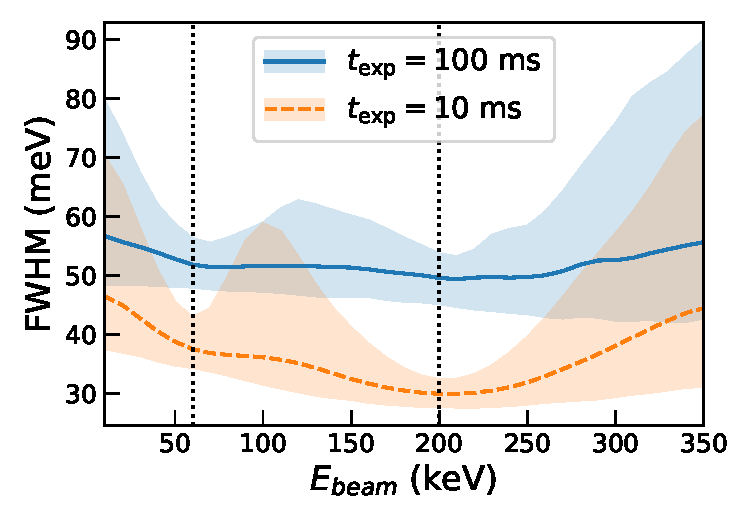
\includegraphics[width=0.49\textwidth]{plots/Ebeam_extrapolation.pdf}
    \includegraphics[width=0.49\textwidth]{plots/time_extrapolation.pdf}
    \caption{\small The model predictions for the FWHM of the zero loss peak
      (and its corresponding uncertainty) as a function of the beam energy $E_b$
      for two values of the exposure time (left panel)
      and as a function of $t_{\rm exp}$ for two values of $E_b$ (right panel).
      %
      The vertical dashed lines indicate the values of the
      corresponding parameter for which training data is available.
    }
    \label{fig:extrapolbeam}
\end{figure}
%%%%%%%%%%%%%%%%%%%%%%%%%%%%%%%%%%%%%%%%%%%%%%%%%%%%%%%%%%%%%%%%%%%%%%%%%%%%%%%%%%%%%%%%%%%%

For this comparison one can observe that as expected the uncertainty in the  prediction for FWHM
of the ZLP is the smallest close to the values of $E_b$ for which one has training data.
%
The uncertainties increase but only in a moderate way in in the interpolation region, indicating that
the model can be reliable applied to predict the features of the ZLP other values of the electron
energy beam (assuming that all other operation conditions of the microscope are unchanged).
%
The errors increase rapidly in the extrapolation region, which is a characteristic feature of
these neural network models.
%
Indeed, as soon as the model departs from the data region there exist a very large
number of different functional form models for $I_{\rm ZLP}(\Delta E)$ that can describe equally well
the training dataset, and hence a blow up of the extrapolation uncertainties is generically expected.

The network was trained on data with exposure times of $10$ and $100$ ms,
so interpolation and extrapolation is possible. Similar to the predictions for varying beam energy, also for exposure time the uncertainties grow bigger as the value deviates more from the training inputs.
%
The right panel of Fig.~\ref{fig:extrapolbeam} displays a similar model
comparison as in the left one but now and as a function of $t_{\rm exp}$ for two values of $E_b$ (right panel).
%
We observe that the FWHM increases roughly in a linear manner with the exposure time, indicating
that lower values of $t_{\rm exp}$ allow for an improved spectral resolution.
%
Further, also in this case we find that the model uncertainties grow rapidly in the
extrapolation region beyond that covered for the training dataset.




% Discussion of the results in sample
\section{Results II. Sample spectra}
\label{sec:results_sample}

Following the discussion of the vacuum ZLP analysis, we now
present the application of our machine learning strategy to parametrise the ZLP
arising in spectra recorded on specimens, specifically for
EELS measurements acquired in different regions
of the WS$_2$ nanoflowers presented in Sect.~\ref{sec:tmd}.
%
The resulting ZLP parametrisation will be applied to isolate the inelastic
contribution in each spectrum.
%
We will use these subtracted spectra first to determine the bandgap type and energy 
value from the behaviour of the onset region and second to identify excitonic
transitions at very low energy losses.

We start this section by presenting the training dataset, which consists of two groups of EEL spectra recorded
in thick and thin regions of the WS$_2$  nanoflowers respectively.
%
Then we discuss the subtraction procedure, the choice of hyper-parameters, and the error propagation
to the physical predictions.
%
The resulting subtracted spectra provide the information
required to extract the value and type of the bandgap
and to characterise excitonic transitions for different regions of these polytypic WS$_2$ nanostructures.


\subsection{Training dataset}
%

Low-magnification TEM images and the corresponding
spectral images of two representative regions of
the WS$_2$ nanoflowers, denoted as sample A and B  respectively, are displayed in Fig.~\ref{fig:ws2positions}.
%
These spectral images have been recorded in the regions marked by a green square
in the associated TEM images, and contain an individual EEL spectrum in each pixel.
%
We indicate the specific locations where
EEL spectra have been recorded, including the in-vacuum measurements acquired
for calibration purposes.
%
Note that in sample B  the differences in contrast are related to the material
thickness, with higher contrast corresponding to thinner regions.

These two samples are characterised by rather different structural morphologies.
%
While sample A is a relatively thick region of WS$_2$, sample B corresponds to a region composed 
of thin petals, which is only one or a few monolayers thick. 
%
In other words, sample A is composed by bulk WS$_2$ while in sample B some specific regions
are much thinner, down to the few monolayers level.
%
This thickness information has been be determined
by means of the {\tt Digital~Micrograph} software.

%%%%%%%%%%%%%%%%%%%%%%%%%%%%%%%%%%%%%%%%%%%%%%%%%%%%%%%%%%%%%%%%%%%%%%%
\begin{figure}[h]
\begin{centering}
  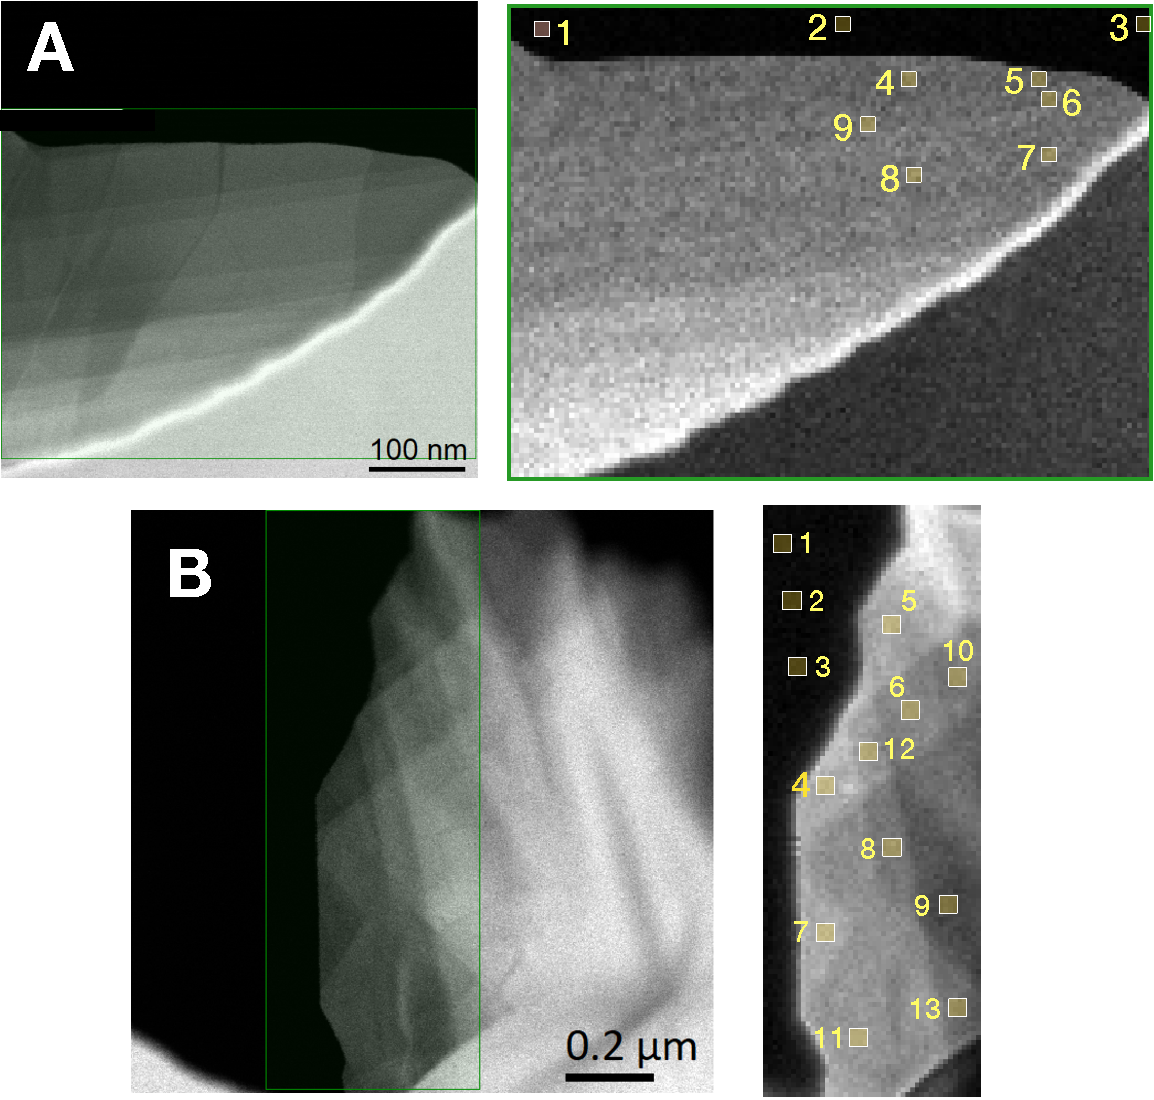
\includegraphics[width=0.87\linewidth]{plots/Spectra_location2.pdf}
  \caption{Low-magnification TEM images (left) and the corresponding
    spectral images (right panels) of two different regions of
    the WS$_2$ nanoflowers, denoted as sample A (upper) and sample B (lower panels) respectively.
    %
    The spectral images have been recorded in the regions marked by a green square
    in the associated TEM images, and contain an individual EEL spectrum in each pixel.
    %
    We indicate the locations where representative
    EEL spectra have been selected. 
    %
    In the left panel of sample B, the difference in contrast is correlated to the material
    thickness, with higher contrast indicating thinner regions of the nanostructure.
    %
    The morphological differences between the two samples are discussed in the text.
  }
\label{fig:ws2positions}
\end{centering}
\end{figure}
%%%%%%%%%%%%%%%%%%%%%%%%%%%%%%%%%%%%%%%%%%%%%%%%%%%%%%%%%%%%%%%%%%%%%%%%%%

One of the main goals of this study is demonstrating that our ZLP-subtraction method leads to
a satisfactory performance for spectra recorded with different microscopes and operating conditions.
%
With this motivation, the EELS measurements acquired on specimens A and B have
been obtained varying both the microscopes and their settings.
%
The TEM and EELS measurements acquired in specimen A  are based on a JEOL 2100F
microscope with a cold field-emission gun and equipped with an aberration corrector,
operated at 60 kV. A Gatan GIF Quantum energy filter was used for
the EELS analysis.
%
The corresponding measurements on specimen B were recorded instead
using a JEM ARM200F monochromated microscope operated at 60 kV, equipped with a GIF quantum ERS filter.
%
See Methods at the end of this work for more details.\\

In Table~\ref{table:sampledata} we collect the most relevant properties of the spectra collected
in the locations indicated in Fig.~\ref{fig:ws2positions} using the same format as
in Table~\ref{table:vacuumdata}.
%
Note that since the spectra from samples A and B
have been acquired with different microscopes, features of the ZLP
such as the FWHM are expected to be different.
%
From this table one can observe how the ZLP for the spectra acquired on sample A exhibit
a FWHM about five times larger as compared to those of sample B.
%
This difference in resolution can be understood from the fact that the EELS spectra from sample B, unlike those
from sample A, were recorded with a TEM equipped with a monochromator.

%%%%%%%%%%%%%%%%%%%%%%%%%%%%%%%%%%%%%%%%%%%%%%%%%%%%%%%%%%%%%%%%%%%%%%%%%%%%%%%%%%%%%%%%%%%%%
%%%%%%%%%%%%%%%%%%%%%%%%%%%%%%%%%%%%%%%%%%%%%%%%%%%%%%%%%%%%%%%%%%%%%%%%%%%%%%%%%%%%%%%%%%%%%
\begin{table}[H]
  \begin{center}
            \renewcommand{\arraystretch}{1.50}
  \begin{tabular}{@{}ccccccccc}
\br
Set & $t_{\rm exp}$ {(}ms{)} & $E_{\rm b}$ {(}keV{)} & $N_{\rm sp}$ & $N_{\rm dat}$ & $\Delta E_{\rm min}$~(eV)  & $\Delta E_{\rm max}$~(eV)  & FWHM~(meV)  \\ 
\mr
A        &       1       &        60         &   6      &    1918    &     -4.1       & 45.5 & $ 470\pm 10$  \\
B        &       190       &        60       &   10     &    2000    &     -0.9        & 9.1   & $ 87 \pm 5$ \\
\br
\end{tabular}
\end{center}
\caption{Same as Table~\ref{table:vacuumdata} now for the EEL spectra taken on specimens A and B.
    %
Note that the location on the WS$_2$ nanoflowers where each spectra has been recorded
was indicated in Fig.~\ref{fig:ws2positions}.}
\label{table:sampledata}
\end{table}
%%%%%%%%%%%%%%%%%%%%%%%%%%%%%%%%%%%%%%%%%%%%%%%%%%%%%%%%%%%%%%%%%%%%%%%%%%%%%%%%%%%%%%%%%%%%%%%%%5
%%%%%%%%%%%%%%%%%%%%%%%%%%%%%%%%%%%%%%%%%%%%%%%%%%%%%%%%%%%%%%%%%%%%%%%%%%%%%%%%%%%%%%%%%%%%%

In the following we will present the results for spectra that are representative
for each of the two samples.
%
The full set of spectra is available together with {\tt EELSfitter},
the code used to produce the results of this analysis,
whose installation
and usage instructions are presented in Appendix~\ref{sec:installation}.

\subsection{Subtraction procedure}

Following the strategy presented in Sect.~\ref{sec:methodology}, again we combine
the N$_{sp}$ spectra recorded over each sample and we determine the 
experimental central values and uncertainties for the training points.
%
Next, we need to determine the choice for hyperparameters $\Delta E_I$ and $\Delta E_{II}$,
as we only want to train on data that is different from zero within uncertainties.
%
As explained in Sect.~\ref{sec:training}, we need the location of the first local minimum
on all the spectra to set a bound for $\Delta E_I$ and $\Delta E_{II}$. 
%
The representative plots can be observed in Fig.~\ref{fig:derivatives} and here it becomes
clear how much information is contained within the intensity derivatives of the spectra.
%
One can observe how the derivatives recorded in vacuum (for both specimens at locations
\#1, \#2 and \#3) are monotonically decreasing and slowly convergate to zero, whereas
the derivatives recorded on different regions of a sample behave very similar, capturing fluctuations
that are typical for the corresponding sample.

%%%%%%%%%%%%%%%%%%%%%%%%%%%%%%%%%%%%%%%%%%%%%%%%%%%%%%%%%%%%%%%%%%%%%%%
\begin{figure}[H]
\begin{centering}
  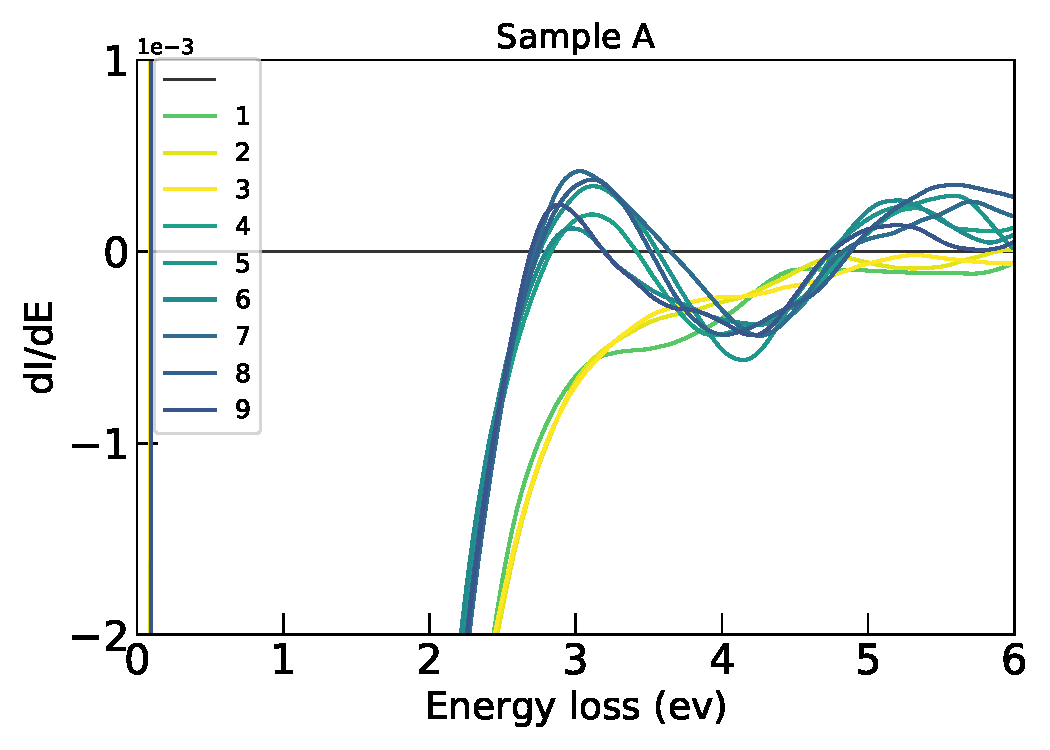
\includegraphics[width=0.49\linewidth]{plots/Derivatives_sample_A.pdf}
  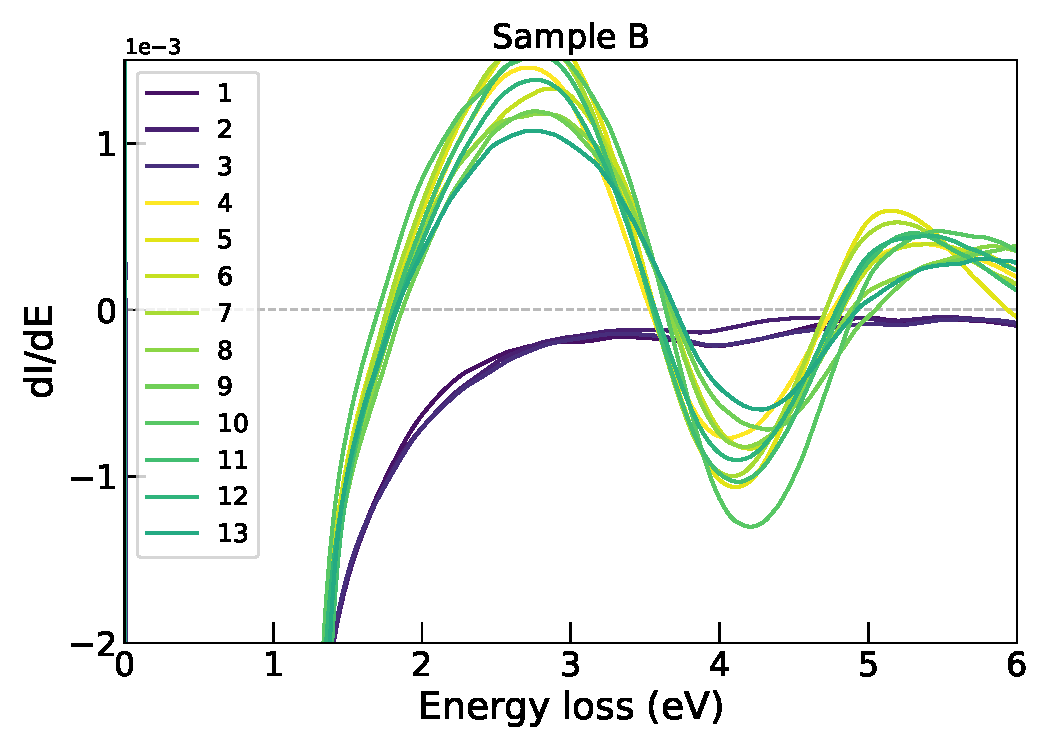
\includegraphics[width=0.49\linewidth]{plots/Derivatives_sample_B.pdf}
  \caption{Plot of the first intensity derivatives of the spectra
  recorded over Sample A (left) and B (right) at the locations
  indicated in Fig.~(\ref{fig:ws2positions}). }
\label{fig:derivatives}
\end{centering}
\end{figure}
%%%%%%%%%%%%%%%%%%%%%%%%%%%%%%%%%%%%%%%%%%%%%%%%%%%%%%%%%%%%%%%%%%%%%%%%%%

\begin{table}[H]
  \begin{center}
            \renewcommand{\arraystretch}{1.50}
  \begin{tabular}{@{}ccccccccc}
\br
Set & $\Delta E|_{\rm min}$~(eV)  &  $\Delta E_{\rm I}$~(eV)  &  $\Delta E_{\rm II}$~(eV)   \\
\mr
A        &    $2.70\pm0.06$               &          1.8        &      12       \\
B        &    $1.80\pm0.04$               &          1.4        &      6        \\
\br
  \end{tabular}
  \end{center}
  \caption{The mean value and uncertainty of the first local minima, $\Delta E|_{\rm min}$,
    averaged over the spectra corresponding to samples A and B from
    Fig.~\ref{fig:ws2positions}.
    %
    We also indicate
    the corresponding values of the hyper-parameters
    $\Delta E_{\rm I}$ and $\Delta E_{\rm II}$ defined in Fig.~\ref{fig:EELS_toy} used for the training
    of the neural network model.
    %
  }
\label{table:sampledata_summary}
\end{table}
%%%%%%%%%%%%%%%%%%%%%%%%%%%%%%%%%%%%%%%%%%%%%%%%%%%%%%%%%%%%%%%%%%%%%%%%%%%%%%%%%%%%%%%%%%%%%%%%%

In Table~\ref{table:sampledata_summary} we have collected the mean value 
and uncertainty of the first local minimum, $\Delta E|_{\rm min}$,
averaged over the spectra corresponding to samples A and B from
Fig.~\ref{fig:ws2positions}.
%
From the uncertainties in $\Delta E|_{\rm min}$, we see that the
location of the first minimum is relatively stable
among all the spectra belonging to a given set.
%
This indicates that the onset of the inelastic contributions $I_{\rm inel}$ does
not change significantly as we move to different regions of the sample.
%
We also indicate
the corresponding values of the hyper-parameters
$\Delta E_{\rm I}$ and $\Delta E_{\rm II}$ defined in Fig.~\ref{fig:EELS_toy}.
%
Recall that only
the data points with $\Delta E \le \Delta E_{\rm I}$ is used for the training
of the neural network model.
%
For $\Delta E \ge \Delta E_{\rm II}$ instead, the training set includes only the pseudo-data
that implements the $I_{\rm ZLP}(\Delta E)\to 0$ constraint.
%
The values for $\Delta E_{\rm II}$ were determined from the vacuum recorded spectra
following the same procedure as explained 
in Sect.~\ref{sec:results_vacuum} and a plot similar to Fig.~\ref{fig:intensityratio} 
can be observed in  Fig.~\ref{fig:pdlocsample}, where we show the ratio between the central
experimental value of the vacuum EEL intensity and their corersponding uncertainty.
%
%%%%%%%%%%%%%%%%%%%%%%%%%%%%%%%%%%%%%%%%%%%%%%%%%%%%%%%%%%%%%%%%%%%%%%%
\begin{figure}[H]
\begin{centering}
  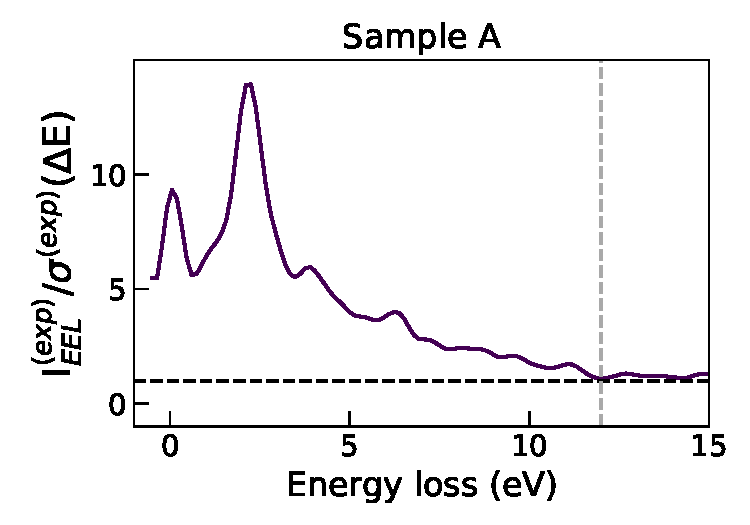
\includegraphics[width=0.49\linewidth]{plots/delta2_sampleA.pdf}
  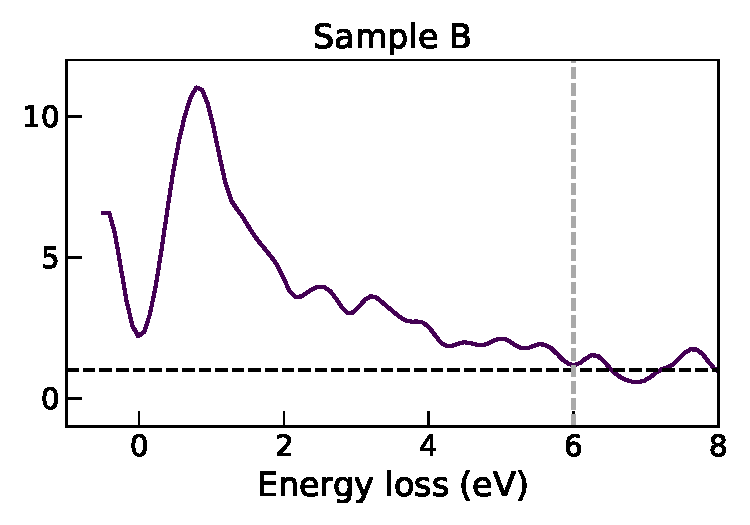
\includegraphics[width=0.49\linewidth]{plots/delta2_sampleB.pdf}
  \caption{The ratio between the central experimental value of the total EELS intensity 
  of the vacuum recorded peaks, I$^{(exp)}_{vac}$,
  and their corresponding uncertainty defined in Eq.~\ref{eq:pdlocation}.
  %
  Results are shown for the mean of the spectra recorded over Sample A (left) and B (right). 
  %
  For both samples, spectrum positions \#1, \#2 and \#3 in Fig.~\ref{fig:ws2positions}
  were used to construct the vacuum central values.
  %
  The vertical dashed lines mark the values of $\Delta E$ for which this ratio becomes smaller 
  than unity, which indicates when the input data starts to be dominated by the statistical noise. 
  }
\label{fig:pdlocsample}
\end{centering}
\end{figure}
%%%%%%%%%%%%%%%%%%%%%%%%%%%%%%%%%%%%%%%%%%%%%%%%%%%%%%%%%%%%%%%%%%%%%%%%%%

We note that the values of $\Delta E_{\rm II}$ for this part are significantly higher than
the ones found in Fig.~\ref{fig:intensityratio}. This could be ascribed to the fact that 
the vacuum spectra from sample A and B are recorded in proximity to a sample, and therefore
effects from the sample are still present, although at a reduced rate.\\

The model training is performed for a range of $\Delta E_{\rm I}$ values
subject to the condition that $\Delta E_{\rm I} \le \Delta E_{\rm min}$.
%
The optimal values of $\Delta E_{\rm I}$ listed in Table~\ref{table:sampledata_summary} are
determined as follows.
%
We evaluate the ratio
between the derivative of the intensity distribution acquired on the specimen over the
same quantity recorded in vacuum,
\be
\label{eq:rder}
\mathcal{R}^{(j)}_{\rm der}(\Delta E) \equiv
\la
\frac{
  dI_{\rm EEL}^{({\rm exp})(j)}(\Delta E)/ d\Delta E
}{
  dI_{\rm EEL}^{({\rm exp})(j')}(\Delta E) /d\Delta E
} \ra_{N_{\rm sp}' } \, ,
\ee
where $j'$ labels one of the $N_{\rm sp}'$ vacuum spectra and the average is taken
over all available values of $j'$.
%
This ratio allows to identify a suitable value of $\Delta E_{I}$ by establishing
for which energy losses the shape (rather than the absolute value) of the intensity distributions 
recorded on the specimen starts to differ significantly from their vacuum counterparts.
%
A sensible choice of $\Delta E_{\rm I}$ could for instance be given by
$\mathcal{R}_{\rm der}(\Delta E_{\rm I}) \simeq 0.9$, for which derivatives differ
at the 10\% level.
%
Note also that the value of the energy loss satisfying
$\mathcal{R}_{\rm der}(\Delta E)=0$ in Eq.~(\ref{eq:rder}) corresponds to the position of the first
local minimum of the spectrum.

For both Sample A and B, the ratios calculated by means of Eq.~(\ref{eq:rder}) 
can be observed in Fig.~\ref{fig:rder} for two representative spectrum locations: 
we have used loc \#4 in both cases. Similar results are obtained for different
positions.

%%%%%%%%%%%%%%%%%%%%%%%%%%%%%%%%%%%%%%%%%%%%%%%%%%%%%%%%%%%%%%%%%%%%%%%
\begin{figure}[H]
\begin{centering}
  \includegraphics[width=0.49\linewidth]{plots/Derivatives_ratio_A.pdf}
  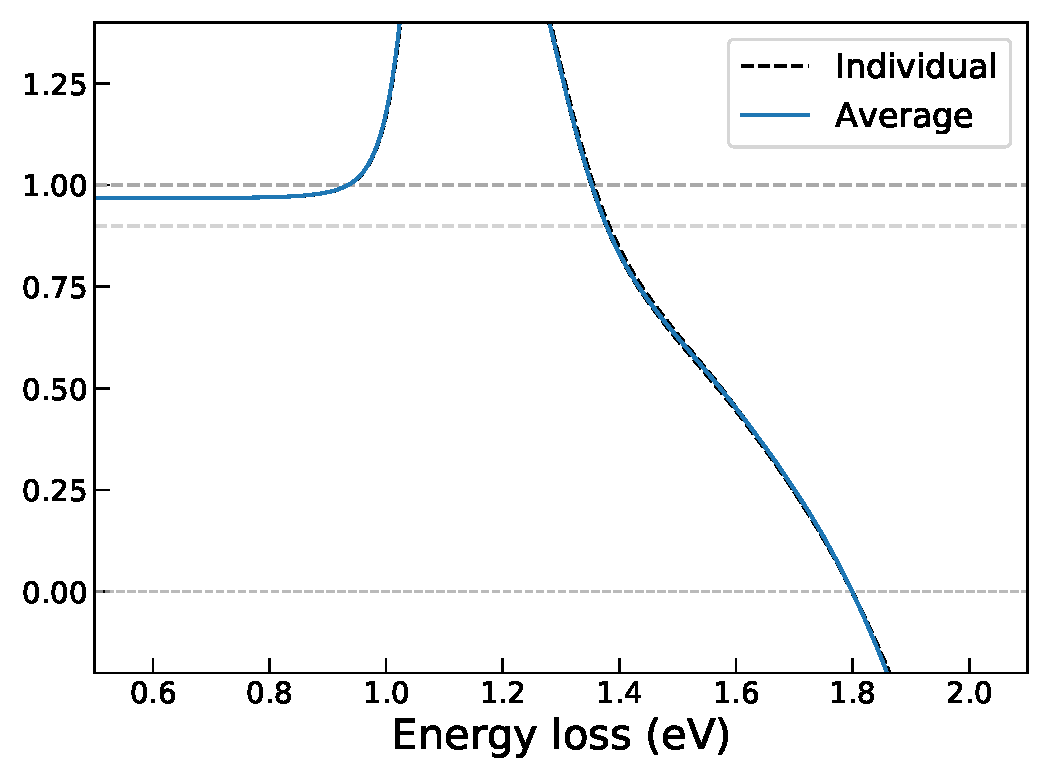
\includegraphics[width=0.49\linewidth]{plots/Derivatives_ratio_B.pdf}
  \caption{Plot of the first intensity derivatives of the spectra
  recorded over Sample A (left) and B (right) at the locations
  indicated in Fig.~(\ref{fig:ws2positions}).}
\label{fig:red}
\end{centering}
\end{figure}
%%%%%%%%%%%%%%%%%%%%%%%%%%%%%%%%%%%%%%%%%%%%%%%%%%%%%%%%%%%%%%%%%%%%%%%%%%

In specimen A it is straightforward to find that $\mathcal{R}_{\rm der}(\Delta E_I) \simeq 0.9$
at an energy loss of 1.8 eV. 
%
For specimen B,  $\mathcal{R}_{\rm der} \simeq 0.9$ at $\Delta E$=1.4 eV.
%
In this case however, the ratio first starts to increase before it decreases again. 
%
This happens consistently for all three vacuum spectra: the three individual ratios can hardly
be distinguished. 
%
It should be noted that the derivatives also differ at the 10\% level when 
$\mathcal{R}_{\rm der} \simeq 1.1$, which corresponds to $\Delta E$=1 eV.
%
Still, we use the point where $\mathcal{R}_{\rm der} \simeq 0.9$
for the determination of $\Delta E_{\rm I}$.
%
The reason to favor this choice over $\mathcal{R}_{\rm der}(\Delta E_I) \simeq 1.1$ is from 
the physical interpretation: after this point,
the derivative of the intensity distributions acquired on samples starts 
to approximate zero much faster than the derivatives in vacuum.
%
when the effect of the sample kicks in, the intensity profile should flatten or increase rather than
continue decreasing, which means the derivatives ratio should be {\it smaller} than unity. 
%
For this reason we choose $\Delta E_I$=1.4 eV as hyper-parameter for specimen B. 
Note that the validity of this choice will be checked later on.\\

Now that we have verified our choices of $\Delta E_I$ and $\Delta E_{II}$ for both samples,
we can move to the results of the training sessions. 
%
The end result of the neural network training is
 a set of $N_{\rm rep}=500$ replicas
  parametrising the ZLP, $I_{\rm ZLP}^{({\rm mod})(k)}(\Delta E)$.
 %
 Taking into account that we have $N_{\rm sp}$ individual spectra in each sample,  the ZLP
 subtraction is performed individually
 for each Monte Carlo replica,
 \be
 \label{eq:subtractedModelPrediction}
 I_{\rm inel}^{({\rm exp})(j,k)}(\Delta E) \equiv I_{\rm EELS}^{({\rm exp})(j)}(\Delta E) - I_{\rm ZLP}^{({\rm mod})(k)}(\Delta E)\, ,
 \quad \forall~N_{\rm rep} \, ,\quad j=1,\ldots,N_{\rm sp} \, ,
 \ee
 from which statistical estimators can be evaluated as usual.
 %
 For instance, the mean value for our model prediction for the $j$-th spectrum
 can be evaluated by averaging over the set of replicas,
 \be
 \la  I_{\rm inel}^{({\rm exp})({\rm (exp)}j)}\ra (\Delta E)
 = \frac{1}{N_{\rm rep}} \sum_{k=1}^{N_{\rm rep}}  I_{\rm inel}^{({\rm mod})(j,k)}(\Delta E) \, ,
 \quad j=1,\ldots,N_{\rm sp} \, ,
 \ee
 and likewise for the corresponding uncertainties or correlations.
%
 For large values of $\Delta E$
 the model prediction reduces to the original spectra, since in that region
 the ZLP contribution vanishes,
 \be
 I_{\rm inel}^{({\rm exp})(j,k)}(\Delta E \gg \Delta E_{\rm I}) \to  I_{\rm EEL}^{{\rm (exp)}(j)}(\Delta E) \, ,\quad
 \forall~j,k \, .
 \ee
 
 For very small values of the energy loss, the contribution to the total
 spectra from inelastic scatterings is negligible
 and thus the subtracted model prediction Eq.~(\ref{eq:subtractedModelPrediction}) should
 be zero. 
 %
 However, this will not be the case in practice since the neural-net model is trained on
 the $N_{\rm sp}$ ensemble of spectra, rather that just on individual ones, and thus the expected
 $\Delta E \to 0$ behaviour will only be achieved within uncertainties rather than at the level of
 central values.
 %
 Therefore, in the zero-loss regime the subtracted spectrum will not vanish completely.
 %
 To achieve the desired $\Delta E \to 0$ limit, we apply a matching procedure
 as follows.
 %
 We introduce another hyper-parameter, $\Delta E_0 < \Delta E_1$, such that
 one has for the $k$-th ZLP replica associated to the $j$-th spectrum the following
 behaviour:
 \bea
 \nonumber
 I_{\rm ZLP}^{({\rm mod})(j,k)}(\Delta E) &=& I_{\rm EELS}^{({\rm exp})(j)}(\Delta E) \, ,\quad \Delta E < \Delta E_0  \, ,\\
 I_{\rm ZLP}^{({\rm mod})(j,k)}(\Delta E) &=& I_{\rm EELS}^{{\rm (exp)}(j)} + \lp \xi_1^{(n_l)(k)}(\Delta E) -
 I_{\rm EELS}^{{\rm (exp)}(j)}(\Delta E)\rp  \times \mathcal{F} \, , \nonumber \quad 
 \Delta E_0 < \Delta E \le \Delta E_1 \, ,\\
 &&\mathcal{F} = \exp\lp -\frac{\lp \Delta E - \Delta E_1 \rp^2 }{\lp \Delta E_0 - \Delta E_1 \rp^2 \delta^2} \rp  \, , \label{eq:matching} \\
 I_{\rm ZLP}^{({\rm mod})(j,k)}(\Delta E) &=& \xi_1^{(n_l)(k)}(\Delta E) \, , \quad \Delta E > \Delta E_1 \nonumber \, .
 \eea
In Eq.~(\ref{eq:matching}), $\xi_1^{(n_l)(k)}$ indicates the output of the $k$-th neural network that parametrises
 the ZLP and $\delta$ is a dimensionless tunable parameter.
 %
This matching procedure might look complex at first sight, however it states just the following:
\begin{itemize}
\item For $\Delta E < \Delta E_0$, the modeled ZLP is exactly the same as the original spectrum;
\item Between $\Delta E_0$ and $\Delta E_1$, the transition sets in to the ZLP model prediction. $\mathcal{F}(\Delta E)$ represents a matching factor
 that ensures that the ZLP model prediction smoothly interpolates
 between $\Delta E=\Delta E_0$ (where $\mathcal{F}\ll 1$ and the original spectrum should
 be reproduced) and $\Delta E=\Delta E_1$
 (where $\mathcal{F}=1$ leaving the neural network output unaffected);
\item At energy loss higher dan $\Delta E_I$, the modeled ZLP is exactly the network prediction.
\end{itemize}

 %
 Here we adopt $\Delta E_0 = \Delta E_1 -0.5\,{\rm eV}$,  having verified
 that results are fairly independent of this choice.
 %
 Taking into account the matching procedure, we can slightly modify Eq.~(\ref{eq:subtractedModelPrediction})
 to 
 \be
 \label{eq:subtractedModelPrediction2}
 I_{\rm inel}^{({\rm mod})(j,k)}(\Delta E) \equiv I_{\rm EELS}^{({\rm exp})(j)}(\Delta E) - I_{\rm ZLP}^{({\rm mod})(j,k)}(\Delta E)\, ,
 \quad \forall~N_{\rm rep} \, ,\quad j=1,\ldots,N_{\rm sp} \, .
 \ee

 The ensemble of ZLP-subtracted spectra $\{I_{\rm inel}^{({\rm mod})(j,k)} \} $
 can then be used to estimate the bandgap of the specimen in the region where
 they were acquired.
 %
 Different approaches  have been put forward to estimate the value of the bandgap from 
subtracted EEL spectra, \textit{e.g.} by means of the inflection point of the rising intensity or
a linear fit to the maximum positive slope~\cite{Schamm:2003}.
%
Here we will adopt the approach of~\cite{Rafferty:2000} where the behaviour
of $I_{\rm inel}(\Delta E)$ in the onset region is modeled as
\begin{equation}
  \label{eq:I1}
    I_{\rm inel}(\Delta E) \simeq  A \lp \Delta E-E_{\rm BG} \rp^{b} \, , \quad \Delta E \ge E_{\rm BG} \, ,
\end{equation}
and vanishes for $E < E_{\rm BG}$, where both the bandgap value
$E_{\rm BG}$ as well as the parameters $A$ and $b$ are extracted from the fit.
%
The exponent $b$ is expected to be $b\simeq 1/2~(3/2)$ for a semiconductor material characterised
by a direct~(indirect) bandgap.
 %
 For each of the $N_{\rm sp}$ spectra and the $N_{\rm rep}$ replicas
 we fit to Eq.~(\ref{eq:subtractedModelPrediction2}) the model Eq.~(\ref{eq:I1})
 within a range taken to be
 $\lc \Delta E_{\rm I} - 0.5~{\rm eV}, \Delta E_{\rm I} + 0.7~{\rm eV}\rc$.
 %
 One ends up with $N_{\rm rep}$ values for
 the bandgap energy and fit exponent for each spectra,
 \be
 \Big \{ E_{\rm BG}^{(j,k)}, b^{(j,k)} \Big\} \, , \quad k=1,\ldots,N_{\rm rep} \, ,
 \quad j=1,\ldots,N_{\rm sp} \, ,
 \ee
 from which again one can readily evaluate their statistical estimators.
 %
 In the following, we will display the median and the 68\% confidence level intervals
 for these parameters to account for the fact that their distribution will be in general non-Gaussian.

 \subsection{Bandgap analysis of sample A}

We present first the results of the bandgap analysis of sample A,
taking location \#4 and \#5 in Fig.~\ref{fig:ws2positions} as representative spectra; 
compatible results are found for the rest of locations.
%
As mentioned above, this region is characterised by a sizable thickness where
WS$_2$ is expected to behave as a bulk material.
%
Fig.~\ref{fig:sp14_subtracted_spectrum} displays the original
and subtracted EEL spectra
together with the predictions of the ZLP model, where
the bands indicate the 68\% confidence level uncertainties and the central value
is the median of the distribution.
%
The inset shows the result of the polynomial fits using Eq.~(\ref{eq:I1}) to the subtracted spectrum
together with the corresponding uncertainty bands.

%%%%%%%%%%%%%%%%%%%%%%%%%%%%%%%%%%%%%%%%%%%%%%%%%%%%%%%%%%%%%%%%%%%%%%%
\begin{figure}[H]
\begin{centering}
  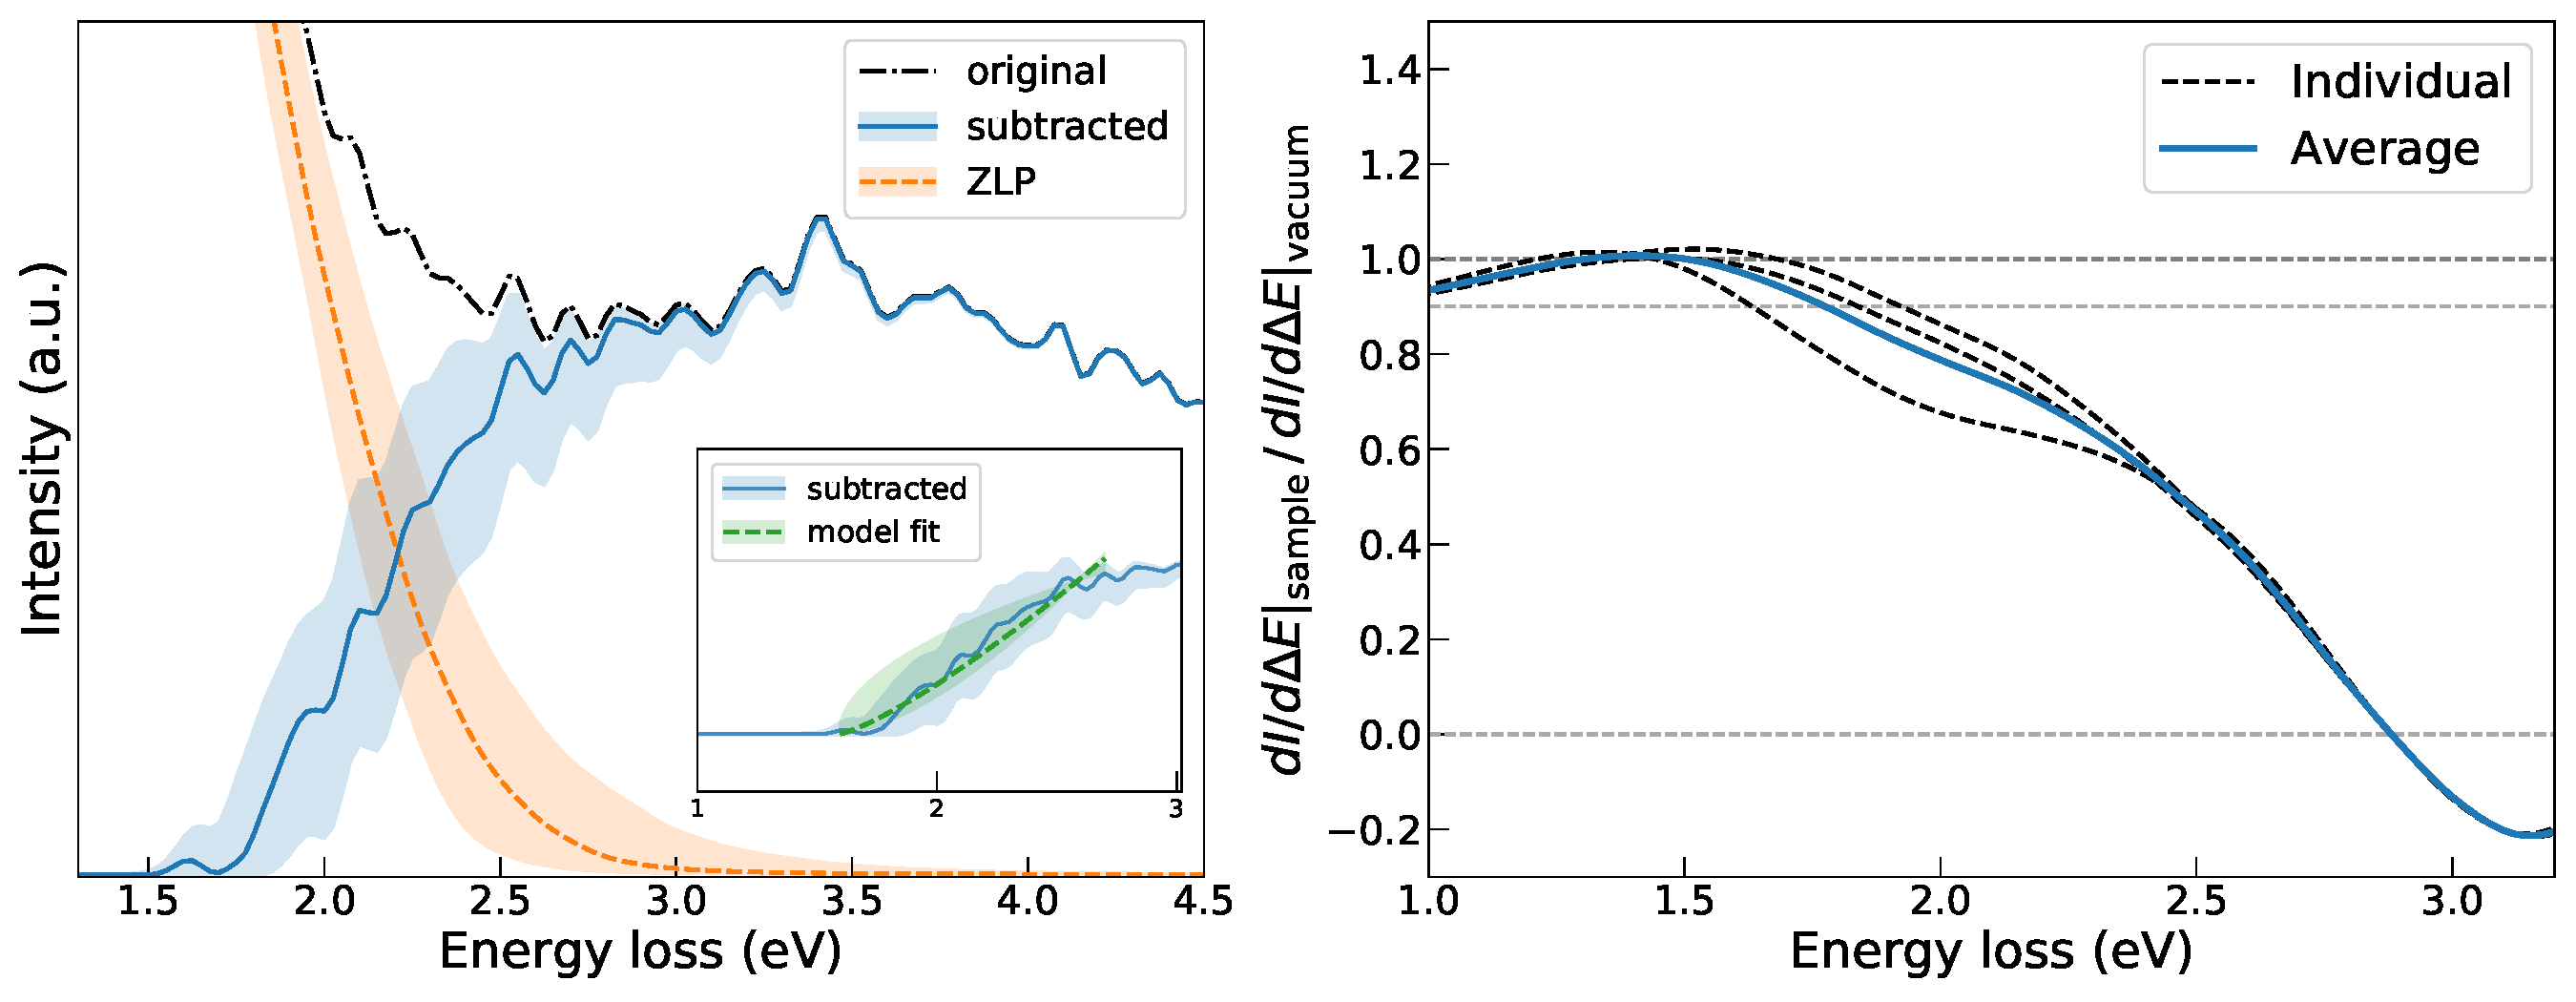
\includegraphics[width=0.49\linewidth]{plots/SubtractedEELS_plot_sp14.pdf}
  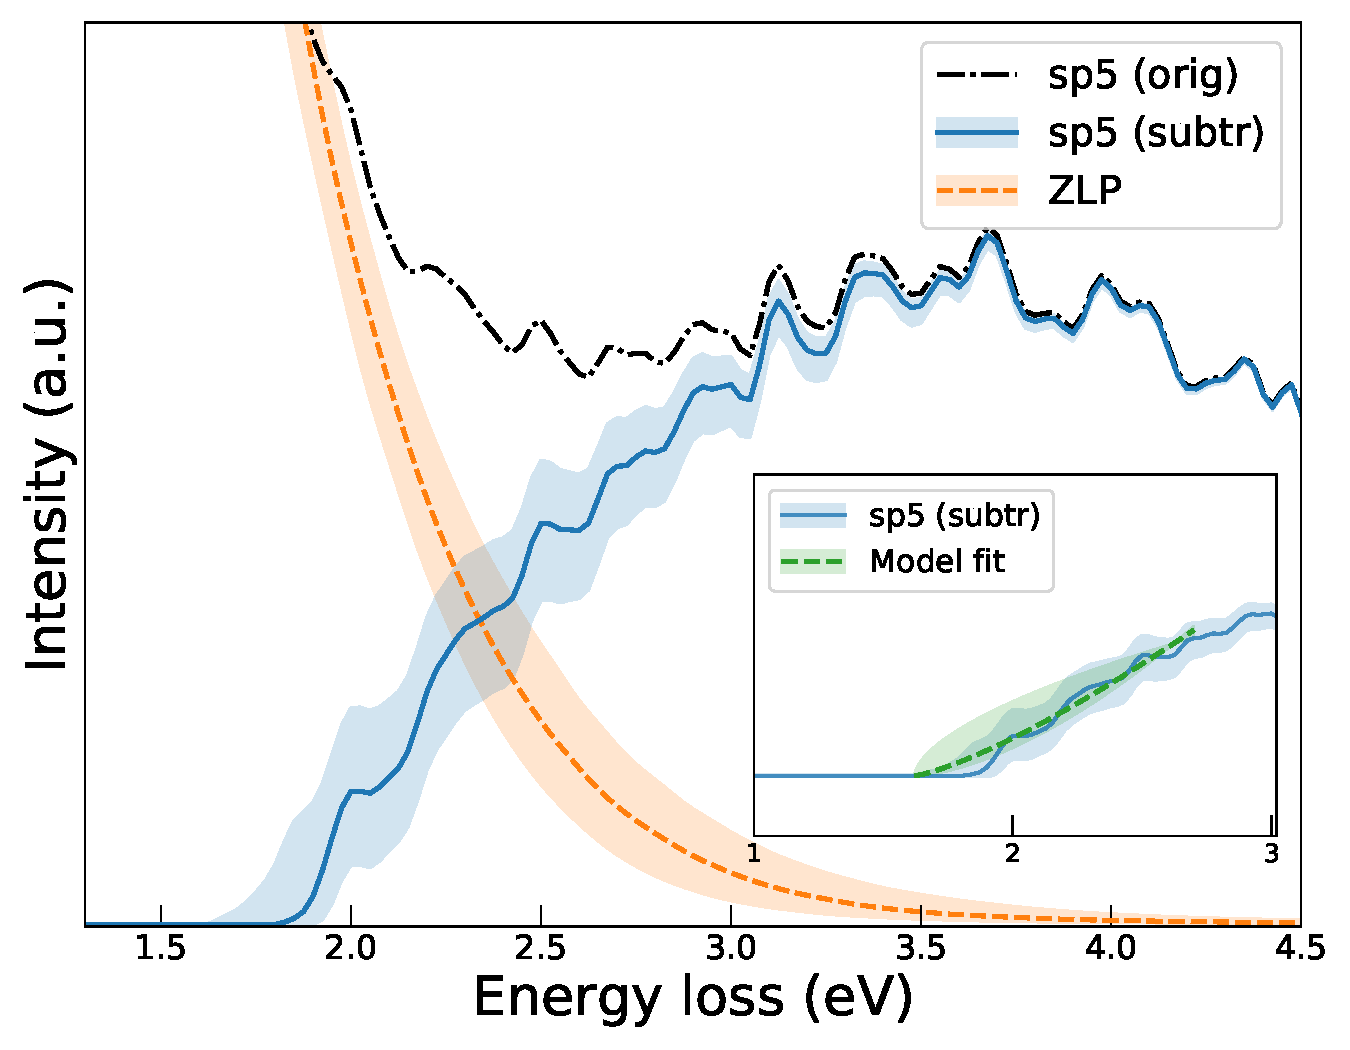
\includegraphics[width=0.49\linewidth]{plots/SubtractedEELS_plot_sp15.pdf}
   \caption{The original
     and subtracted EEL spectrum corresponding to location \#4 (left) and \#5 (right)
     of sample A in Fig.~\ref{fig:ws2positions},
     together with the predictions of the ZLP model, where
     the bands indicate the 68\% confidence level uncertainties.
     %
     The inset displays the result of fitting Eq.~(\ref{eq:I1}) to the onset
     region of the subtracted spectrum.
  }
\label{fig:sp14_subtracted_spectrum}
\end{centering}
\end{figure}
%%%%%%%%%%%%%%%%%%%%%%%%%%%%%%%%%%%%%%%%%%%%%%%%%%%%%%%%%%%%%%%%%%%%%%%%%%

One can observe how the ZLP model uncertainties are small at low $\Delta E$
(due to the matching condition) and large $\Delta E$ (where the ZLP vanishes),
but become significant in the intermediate region where the contributions
from $I_{\rm ZLP}$ and $I_{\rm inel}$ become comparable.
%
It is worth emphasizing that these (unavoidable) uncertainties are neglected in most
ZLP subtraction methods, and this is therefore the power of this method.
%
The validity of our choice for the hyperparameter $\Delta E_{\rm I}$ (Table~\ref{table:sampledata_summary})
can be verified {\it a posteriori} by evaluating the ratio
\be
\mathcal{R}^{(j)}_{\rm abs}\lp \Delta E_{\rm I}\rp \equiv 
\la I_{\rm ZLP}^{({\rm mod})(j)}\ra_{\rm rep} \Big/I_{\rm EEL}^{({\rm exp})(j)} \Big|_{\Delta E = \Delta E_{\rm I}} \, ,
\ee
which in this case turns out to be $\mathcal{R}_{\rm abs} = 0.98$.
%
It is important to verify that $\mathcal{R}_{\rm abs}\lp \Delta E_1\rp$ is not too far from unity,
indicating that the training dataset has not been contaminated by the inelastic contributions.
%
By requiring that $\mathcal{R}^{(j)}_{\rm der}(\Delta E_{\rm I})\simeq 0.9$ we obtain
the value $\Delta E_{\rm I}=1.8$ eV, which is used as baseline for the analysis.
%
It should be noted that this choice is not unique, for example requiring
$\mathcal{R}^{(j)}_{\rm der}(\Delta E_{\rm I})\simeq 0.8$ instead would have led
to $\Delta E_{\rm I}=2.0$ eV.
%
It is therefore important to asses the stability of our results when the hyper-parameter $\Delta E_{\rm I}$
is varied around its optimal value.

With this motivation, we have performed the training over the EEL spectra 
for a range of $\Delta E_{\rm I}$ values to assess the stability of our
results.
%
In Fig.~\ref{fig:bvalues_sampleA} we display the
values of the exponent $b$
and the bandgap energy $E_{\rm BG}$ 
obtained from spectrum \#4 (left panel in Fig.~\ref{fig:sp14_subtracted_spectrum})
for variations of $\Delta E_{\rm I}$ around its optimal value
(1.8 eV, indicated by the horizontal dashed line) by an amount
of $\pm 0.2$ eV.
%
The central value and the error band for each value of $\Delta E_I$ is evaluated
as the median and the 68\% CL interval over the $N_{\rm rep}=500$ Monte Carlo replicas.
%
We observe that the fit parameters for both $b$ and $E_{\rm BG}$ are stable with respect
to variations of $\Delta E_I$, with any shift in the central value contained within the
uncertainty bands.
%
We can therefore conclude that our approach is robust with respect to the choice of its
hyper-parameters.


%%%%%%%%%%%%%%%%%%%%%%%%%%%%%%%%%%%%%%%%%%%%%%%%%%%%%%%%%%
\begin{figure}[H]
\begin{centering}
  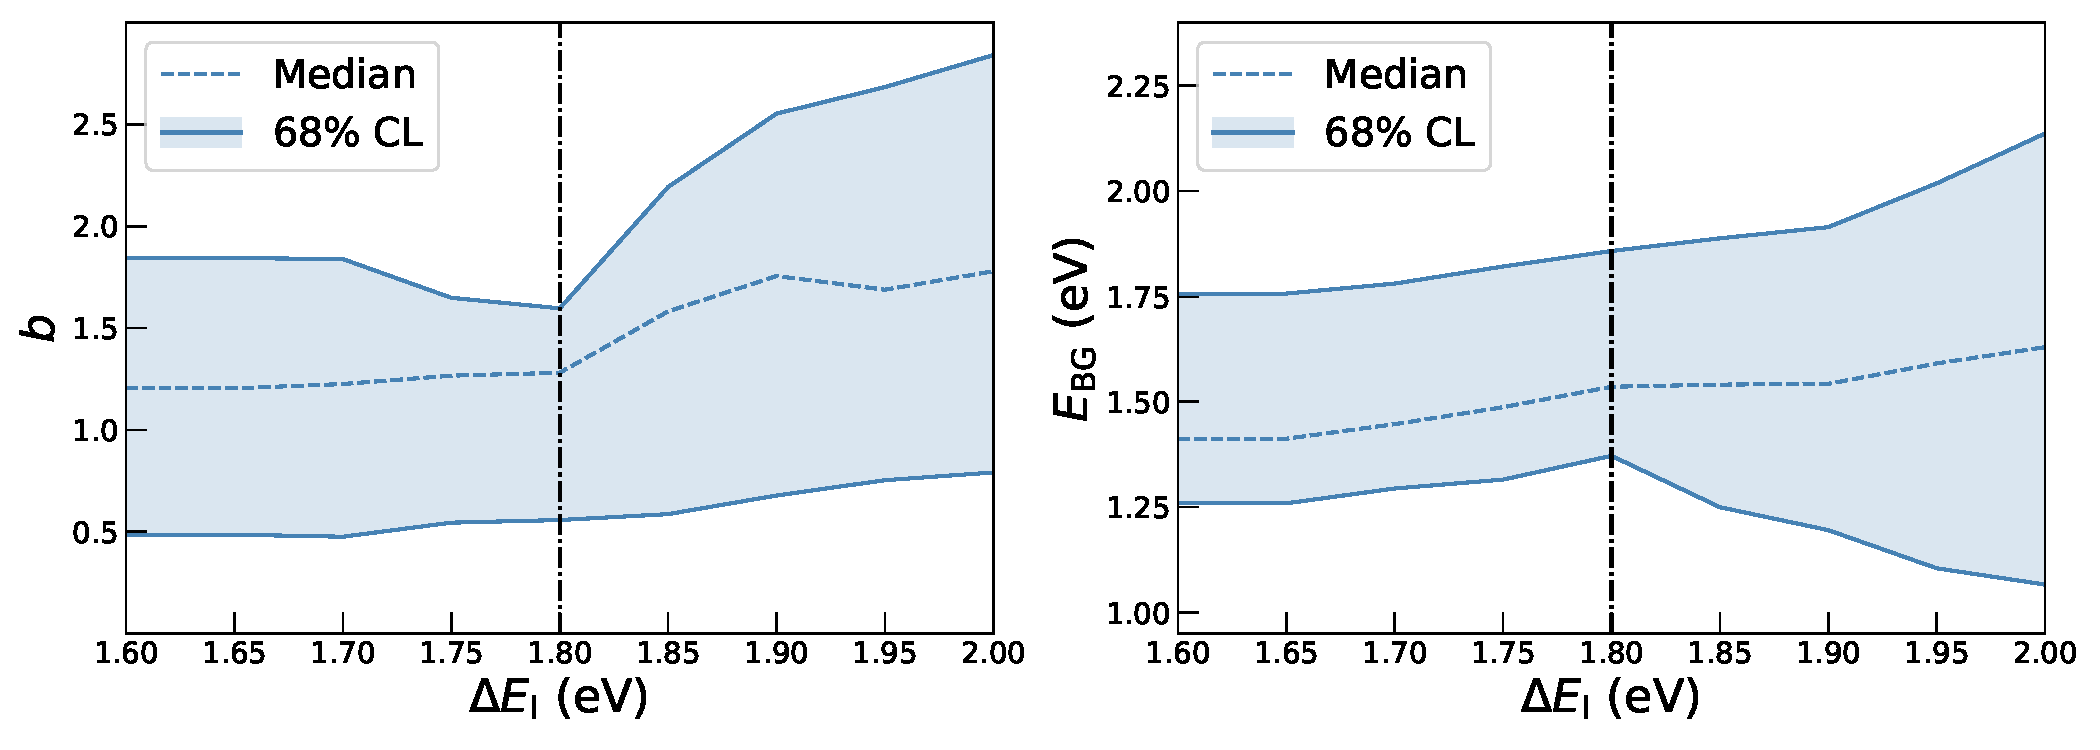
\includegraphics[width=0.99\linewidth]{plots/Stability_plots_sp14_smooth.pdf} 
  \caption{\small The values of the exponent $b$ (left)
    and the bandgap energy $E_{\rm BG}$ (right panel) from the model Eq.~(\ref{eq:I1})
    obtained from the subtracted spectrum sp14 as $\Delta E_{\rm I}$ is varied by $\pm 0.2$ eV
    around its optimal value, indicated by the horizontal dashed line.
  }
\label{fig:bvalues_sampleA}
\end{centering}
\end{figure}
%%%%%%%%%%%%%%%%%%%%%%%%%%%%%%%%%%%%%%%%%%%%%%%%%%%%%%%%%%%%%


The final values for $E_{\rm BG}$ and $b$ obtained in the analysis for spectrum 4 and 5 are
\bea
E_{\rm BG}^{(4)} = 1.6_{-0.2}^{+0.3}\,{\rm eV} \, ,\quad b^{(4)} = 1.3_{-0.7}^{+0.3} (\#4)  \, ,\\
E_{\rm BG}^{(5)}  = 1.6_{-0.2}^{+0.2}\,{\rm eV} \, ,\quad b^{(5)} = 1.3_{-0.5}^{+0.3} (\#5) \, .
\eea
We thus find that for this specific region of the WS$_2$ nanoflowers
the model fit to the subtracted EEL spectrum exhibits a clear preference
for an indirect bandgap (where $b\simeq 1.5$), though a direct one ($b\simeq 0.5$)
cannot be excluded within uncertainties.
%
This result is consistent with the theoretical expectations of the local
electronic properties of bulk WS$_2$.
%
Further, the value of $E_{\rm BG}$ is consistent with previous determinations
in the same material at the bulk level, such as those collected in Table~\ref{table:bgvalues}.
%
Consistent results are obtained for other locations of Fig.~\ref{fig:ws2positions}
where spectra have been recorded. 
%
To demonstrate this, we show in Fig.~\ref{fig:bgstability} the fitted values 
for $E_{\rm BG}$ and $b$ for all spectra 
in Sample A, all evaluated using $\Delta E_I$=1.8 eV for the model training.
%
The uncertainty of the bandgap fit varies between the spectra, however
what is important is the fact that central values are stable within 
uncertainty bands.
%
This implies that we find a consistent favor for an indirect bandgap for each of
the locations on Sample A, which is what we would expect from 
theoretical expectations of bulk WS$_2$.
%
To the best of our knowledge
these results represent the first EELS bandgap analysis of WS$_2$ nanostructures
whose crystalline structure is based on mixed 2H/3R polytypes.

%%%%%%%%%%%%%%%%%%%%%%%%%%%%%%%%%%%%%%%%%%%%%%%%%%%%%%%%%%
\begin{figure}[H]
\begin{centering}
  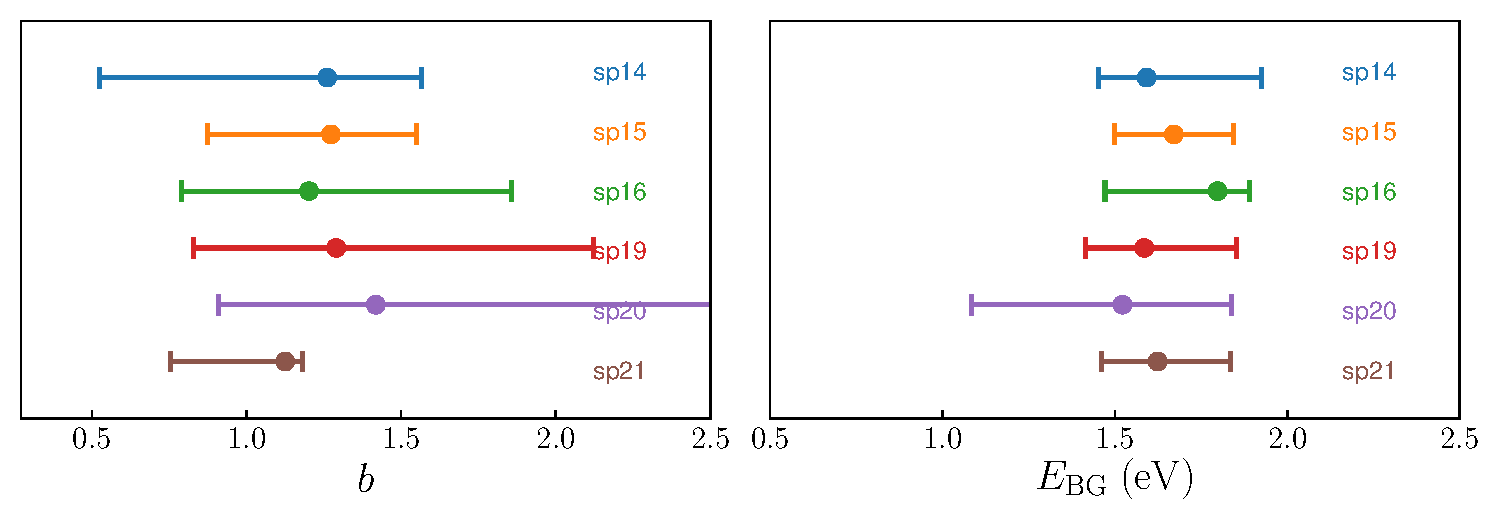
\includegraphics[width=0.9\linewidth]{plots/bg_stability.pdf} 
  \caption{The values of the exponent $b$ (left)
    and the bandgap energy $E_{\rm BG}$ (right panel) from the model Eq.~(\ref{eq:I1})
    obtained from all the subtracted spectra in Sample A, 
    for $\Delta E_{\rm I}$ at its optimal value (1.8 eV). 
  }
\label{fig:bgstability}
\end{centering}
\end{figure}
%%%%%%%%%%%%%%%%%%%%%%%%%%%%%%%%%%%%%%%%%%%%%%%%%%%%%%%%%%%%%


\subsection{Bandgap analysis of sample B}

We now discuss the results of the bandgap analysis of sample B,
taking location sp4 in Fig.~\ref{fig:ws2positions} as representative spectrum; compatible results
are found for the rest of locations.
%
In Fig.~\ref{fig:SubtractedEELS_plot_sp4} we present the analogous
result to that of Fig.~\ref{fig:sp14_subtracted_spectrum}.

%%%%%%%%%%%%%%%%%%%%%%%%%%%%%%%%%%%%%%%%%%%%%%%%%%%%%%%%%%%%%%%%%%%%%%%
\begin{figure}[H]
\begin{centering}
  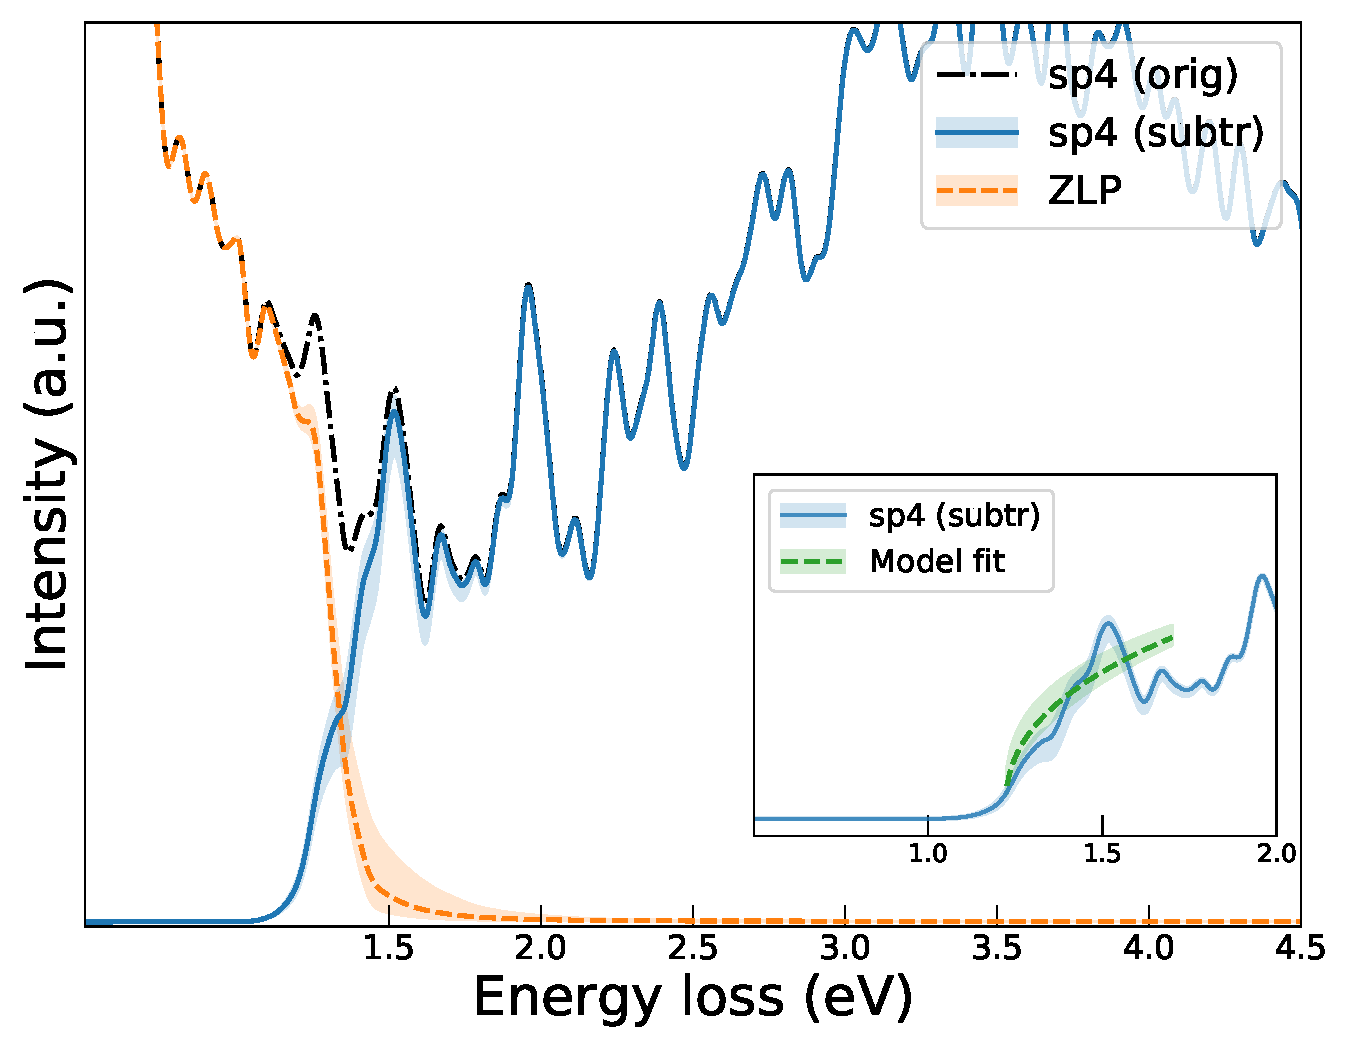
\includegraphics[width=0.60\linewidth]{plots/SubtractedEELS_plot_sp4.pdf}
  \caption{Same as Fig.~\ref{fig:sp14_subtracted_spectrum}
    now for sp4 (sample B) from Fig.~\ref{fig:ws2positions}.
  }
\label{fig:SubtractedEELS_plot_sp4}
\end{centering}
\end{figure}
%%%%%%%%%%%%%%%%%%%%%%%%%%%%%%%%%%%%%%%%%%%%%%%%%%%%%%%%%%%%%%%%%%%%%%%%%%

Fig.~\ref{fig:subtracted_spectra_comp} displays the
the ZLP-subtracted spectra from sample B corresponding to locations sp4, sp5, and sp6
    from Fig.~\ref{fig:ws2positions} together with the corresponding model uncertainties.
    %
    Results are shown for two values of the hyperparameter $\Delta E_{\rm I}$,
    1.45 eV (left) and 1.55 eV (right panel).
    %
    Note how features of the subtracted spectra such as the peaks as $\Delta E\simeq 1.5$,
    1.7 and 2.0 are common across the three spectra, demonstrating that there
    are genuine physical features of the ultra-low-loss region rather than statistical
    fluctuations.
    %
The research on fundamental optical properties of TMDs has led to the discovery of different 
types of exciton transitions in the ultra-low-loss region of WS$_2$ nanostructures. 
%
The origin of these peaks can be attributed to the formation of an electron-hole pair mitigated
by the dielectric screening from the surrounding lattice~\cite{Hanbicki:2016}.
%
In reduced dimensions as in single layers of TMDs, exciton peaks arise with binding energies
up to ten times larger than for bulk structures.
%
In the optical spectra of TMDs, two strongly pronounced resonances denoted by A and B
excitons are often observed, appearing at binding energies of 300-500 meV below the true band gap~\cite{Karivaj:2019}.
%
This is in accordance with the features observed in Fig.~\ref{fig:subtracted_spectra_comp} at 
$\Delta E\simeq 1.5$ and 1.7 eV, which is exactly 300-500 meV below the true bandgap value
expected for 2D structures of WS$_2$. 
%
The presence of these low loss features makes the bandgap analysis on this sample 
non-trivial, since one can only fit Eq.~(\ref{eq:I1}) to the onset region of the 
bandgap excitation. 
%
Nevertheless, the ZLP-subtracted spectra in Fig.~\ref{fig:subtracted_spectra_comp} show that
we have been able to cleanly resolve exciton features down to 1.5 eV within appropriate
uncertainty.

%%%%%%%%%%%%%%%%%%%%%%%%%%%%%%%%%%%%%%%%%%%%%%%%%%%%%%%%%%%%%%%%%%%%%%%
\begin{figure}[H]
\begin{centering}
  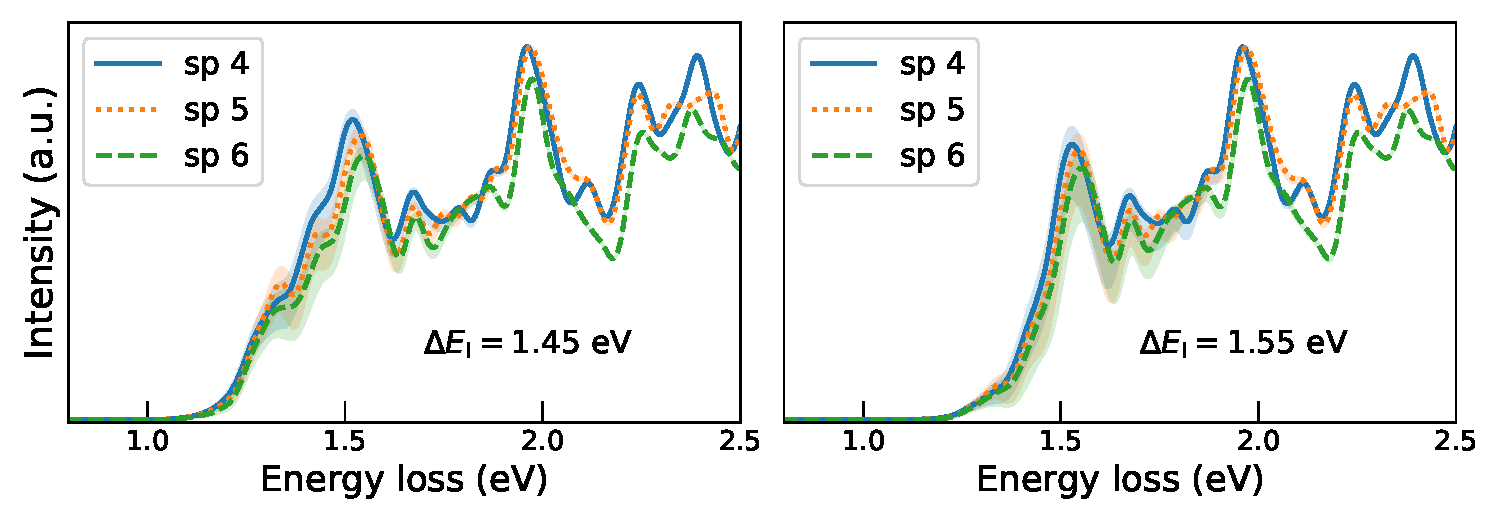
\includegraphics[width=0.99\linewidth]{plots/subtracted_spectra_comp.pdf}
  \caption{The ZLP-subtracted spectra from sample B corresponding to locations sp4, sp5, and sp6
    from Fig.~\ref{fig:ws2positions} together with the corresponding model uncertainties.
    %
    Results are shown for two values of the hyperparameter $\Delta E_{\rm I}$,
    1.45 eV (left) and 1.55 eV (right panel).
    %
    Note how features of the subtracted spectra such as the peaks as $\Delta E\simeq 1.5$,
    1.7 and 2.0 are common across the three spectra.
  }
\label{fig:subtracted_spectra_comp}
\end{centering}
\end{figure}
%%%%%%%%%%%%%%%%%%%%%%%%%%%%%%%%%%%%%%%%%%%%%%%%%%%%%%%%%%%%%%%%%%%%%%%%%%





% Summary and outlook
%%%%%%%%%%%%%%%%%%%%%%%%%%%%%%%%%%%%%%%%%
\section{Summary and outlook}
%%%%%%%%%%%%%%%%%%%%%%%%%%%%%%%%%%%%%%%%%
\label{sec:summary}

In this work we have presented a novel, model-independent strategy to parametrise and subtract
the omnipresent zero-loss peak that dominates the low-loss region
of EEL spectra.
%
Our strategy is based on machine learning techniques and provides a faithful estimate of the
uncertainties associated to both the input data and the procedure itself,
which can  then be propagated to physical predictions without any assumptions or approximations.
%
We have demonstrated how, in the case of vacuum spectra, our approach
is sufficiently flexible to accomodate several input variables corresponding
to different operating conditions of the microscope, such as the exposure time and beam energy.
%
Further, we are able to reliably interpolate and
extrapolate our predictions, {\it e.g.} for the expected FWHM of the ZLP,
to operating conditions not included in the training dataset.
%
When applied to spectra recorded on specimens, our approach
makes it possible to robustly disentangle the ZLP contribution from
those arising from inelastic interactions with the sample.
%
Thanks to this subtraction procedure, one can fully exploit
the valuable physical information contained in the ultra low-loss region of
the spectra. \\

As a proof of concept, we have applied the ZLP subtraction
strategy to EEL spectra recorded in two samples of WS$_2$ nanoflowers characterised by a
2H/3R polytypic crystalline structure.
%
Measurements taken in the first sample, representing a relatively thick region of WS$_2$ (bulk material),
were used to determine
the local value of the bandgap energy $E_{\rm BG}$
and to assess whether the nature of this bandgap is direct or indirect.
%
A model fit to the onset of the inelastic intensity distribution leads to
a bandgap energy
$E_{\rm BG} \simeq 1.6^{+0.3}_{-0.2}\,{\rm eV}$ and 
exhibits a clear preference for an indirect bandgap.
%
Our findings are consistent with previous studies, both of theoretical
and of experimental nature, concerning the bandgap structure of bulk WS$_2$.

Subsequently, we have applied our method to a thinner sample of the WS$_2$ nanoflowers,
specifically a region composed by overlapping petals with varying
thicknesses that can be as small as a few monolayers.
%
We have demonstrated how for such specimens one can exploit the ZLP-subtracted results
to characterise the local excitonic transitions that arise in the ultra-low-loss region.
%
By charting the bandgap region region of 2H/3R polytypic WS$_2$,
we identify two strong peaks at $\Delta E\simeq 1.5$ and 2 eV
(and a softer one at 1.7 eV) and we show how
these features are consistent when comparing
spatially-separated locations in sample B, 
independent of our choice of hyper-parameters.

The power of this method is that it provides an associated uncertainty estimate,
which makes it possibile to robustly establish the statistical significance
of each of these features in the ultra-low-loss region.\\

The approach presented in this work could be extended
in several directions.
%
First of all, it would be interesting to test its robustness when additional
operating conditions of the microscope are included as input variables,
{\it e.g.} arperture width or temperature,
and to verify to which extent the ZLP parametrisations obtained for an specific microscope
can be generalised to a completely different TEM.
%
Further, a non-trivial cross-check of our method would be to validate
our predictions for other operating conditions of the microscope with actual measurements, such
as the FWHM as a function of the beam energy $E_b$ or the exposure time
$t_{\rm exp}$ as shown in Fig.~\ref{fig:extrapolbeam}.

Concerning the physical interpretation of the low-loss region of EEL
spectra, our method could be applied to study the bandgap properties 
for different types
of nanostructures built upon TMD materials, such as MoS$_2$ nanowalls~\cite{nanowalls}
and vertically-oriented nano-sheets~\cite{Bolhuis:2020}.
%
It would also be interesting to use a sample which is known to exhibit
a direct bandgap without dominating excitonic transitions in the low-loss regime, 
to verify that the bandgap fitting procedure works 
also for this case.
%
In addition to bandgap characterisation, this ZLP-subtraction
strategy should allow the detailed study
of other phenomena relevant for the interpretation of the low-loss
region such as plasmons, excitons, phonon interactions, and
intra-band transitions.
%
Once could also further exploit the observed peaks in the ultra-low-loss
regime in WS$_2$ monolayers, infer their binding energies
and verify if these peaks indeed correspond to the expected
exciton transitions.
%
Furthermore, the subtracted EEL spectra can be used to further characterise
local electronic properties by means of the
evaluation of the dielectric function and its associated
uncertainties in terms of the Kramers-Kronig relations.

Another possible application of the strategy presented in this work would be the automation of
the study of spectral TEM images,
such as those displayed in the right panels of Fig.~\ref{fig:ws2positions},
where each pixel contains an individual EEL spectrum.
%
Here machine learning methods would provide a useful automated method
to identify relevant features of the spectra with minimal
human intervention, since there is no need to process each spectrum individually.
%
It can then be used to map
the evolution of these features as we move along different regions of the
nanostructure.
%
Such an approach would combine two important families of machine learning algorithms: 
regression, in order to quantify the properties of spectral
features such as width and significance, and classification, to identify categories
of features across the spectral image.

\newpage
\section*{Methods}

{The EEL spectra used for the training of the vacuum ZLP model presented in Sect.~\ref{sec:results_vacuum} 
were collected in a ARM200F Mono-JEOL microscope equipped with a GIF continuum spectrometer and operated at 
60 kV and 200 kV. 
%
For these measurements, a slit in the monochromator of 2.8 $\mu$m was used.
%
The TEM and EELS measurements acquired in Specimen A for the results presented in
Sect.~\ref{sec:results_sample} were recorded in a JEOL 2100F microscope with a cold field-emission
gun equipped with aberration corrector operated at 60 kV. A Gatan GIF Quantum was used for
the EELS analyses. The convergence and collection semi-angles were 30.0 mrad and 66.7 mrad respectively.
%
The TEM and EELS measurements acquired for Specimen B in Sect.~\ref{sec:results_sample}
were recorded using a JEM ARM200F monochromated microscope operated at 60 kV and equipped with
a GIF quantum ERS. The convergence and collection semi-angles were 24.6 mrad and 58.4 mrad respectively
in this case, and the aperture of the spectrometer was set to 5 mm.}




\appendix
%\vspace{1cm}
%\hrule
%\vspace{1cm}

\clearpage
\begin{center}
  {\bf \LARGE Supplementary Material}
 \end{center}

\section{Installation and usage of {\tt EELSfitter}}
\label{sec:installation}

In this appendix we provide some instructions about the installation
and the usage of the {\tt EELSfitter} code developed
in this work.
%
The code is available from its GitHub repository
\begin{center}
\url{https://github.com/LHCfitNikhef/EELSfitter}
\end{center}
and is composed by a number of {\tt Python} scripts.
%
The code requires a working installation of {\tt Python3} and the following
libraries: {\tt NumPy}, {\tt TensorFlow} (v2), {\tt pandas}, {\tt SciPy} and {\tt scikit-learn}.  


\noindent
\paragraph{\tt Load\_data.py}
%
This script reads the spectrum
intensities and create data-frames to be used for training the neural network.
%
It reads out the EEL spectra intensities, automatically selects the energy loss
at which the peak intensity occurs and shifts the dataset such that
the peak intensity is centered at $\Delta E =$0. 
%
Further, for each spectrum it returns the normalized intensity by normalizing
over the total area under the spectrum. 
%
The output is two datasets, {\tt df} and {\tt df\_vacuum} which contain the 
information on the in-sample and in-vacuum recorded spectra respectively. 
%
The user needs to upload the spectral data in .txt format to the 'Data' folder
and make sure that the vacuum and in-sample spectra are added to the appropriate one.
%
For each of the spectra the minimum and maximum value of the recorded energy 
loss need to be set manually in {\tt Eloss\_min} and {\tt Eloss\_max}.

\noindent
\paragraph{\tt Fitter.ipynb}
%
This script is used to run the neural network training on the data that was 
uploaded using {\tt load\_data.py}.
%
It involves a number of pre-processing steps to determine the hyper-parameters $\Delta E_{\rm I}$
and $\Delta E_{\rm II}$ and then
it automatically prepares and cuts the data before it is fed
to the neural network to start the training.
%
It is structured as follows:

\begin{itemize}
  
\item {\it Importing libraries and spectral data} from the {\bf load\_data.py} script.

\item {\it Evaluate  $\Delta E_{\rm I}$ from the intensity derivatives}.
  %
  In order to determine the value for the hyper-parameter
  $\Delta E_{\rm I}$, a dataframe {\tt df\_dx} is created
and it calculates the derivatives of each of the in-sample recorded spectra, 
stored as {\tt df\_dx['derivative y*']}, where {\tt *} is any of the in-sample recorded spectra.
%
The first crossing of any of the derivatives with zero is determined 
and stored as the value of $\Delta E_{\rm I}$. 

\item {\it Evaluate $\Delta E_{\rm II}$ for the pseudo-data.}
  %
It calculates the mean over all vacuum spectra, {\tt df\_mean}, and the ratio of the 
intensity to the experimental uncertainty for each value of
$\Delta E$, {\tt df\_mean['ratio']}. 
%
The value of $\Delta E_{\rm II}$ is then determined as the energy loss at which this ratio
drops below 1 and  is stored together with the value of $\Delta E_{\rm I}$
as the hyper-parameters for training. 
%
However, if one wishes to use other values for these parameters, for instance for 
cross-validating the best value for $\Delta E_{\rm I}$, these can also be adjusted manually.

\item {\it Experimental data processing.}
%
  The next step is to keep only
  the data points with $\Delta E \le \Delta E_{\rm I}$  
and dropping the points with higher energy losses.
%
Experimental central values and uncertainties are calculated by means of equal width 
discretization, for which the number of bins has to be set as {\tt nbins}. 
%
The default value is 32, which means that 32 training inputs are spread equally
over the range [$ \Delta E_{\rm min}, \Delta E_{\rm I}$]. 
%
Note that the logarithm of the intensity is used as training inputs, because this facilitates
the optimization of the neural network ($I_{\rm EEL}$ being a steeply falling function
of $\Delta E$).
%
The code translates this back to the original intensity values after the training.
%
$N_{\rm pd}$
pseudo datapoints are added in the range $[\Delta E_{\rm II}, \Delta E_{\rm max}]$, where
$ \Delta E_{\rm max}$
is the maximum energy loss value of the recorded spectra. 
%
The values for $N_{\rm pd}$ and $\Delta E_{\rm max}$ should be changed manually by 
setting them in {\tt max\_x} and {\tt N\_pseudo}. 
%
The output is a dataframe {\tt df\_full} containing all training data and pseudo data points, 
corresponding to a total of $N_{\rm in}$ (= $n_{\rm bins}$ + $N_{\rm pd}$) training inputs.

\item {\it Initialize the NN model,} where the code
  defines the neural network architecture and prepares the
data inputs to feed them to the neural network for training. 
%
The function {\tt make\_model()} allows to define the number of hidden layers and 
nodes per layer. The default  architecture is 1-10-15-5-1.

\item {\it Initialize data for NN training.}
  %
  Here the code prepares the recorded spectra to be used
as inputs for the neural network. 
%
First, we initiate placeholders for the variables
{\tt x}, {\tt y} and {\tt sigma} which
allow us to create our operations and 
build our computation graph, without needing the data itself. 
%
The dimension of the placeholder is defined by {\tt $[{\bf None}, dim]$} where 'dim'
should be set to the dimension of the corresponding variable. In this case the input is 
one-dimensional, so dim=1. 
%
These placeholders are used to define {\tt predictions}, which is in fact a placeholder that is used 
later to make predictions on inputs {\tt x}. 
%
Also, we define a vector {\tt predict\_x} that is used to make a direct prediction after training
on each of the replicas. It consists of $N_{\rm pred}$ data points in the energy loss range
{\tt [pred\_min, pred\_max]}. 

\item {\it Create the Monte Carlo replicas.}
  %
  The final step to be taken before we can start training is the creation of
  sample of $N_{\rm rep}$ Monte Carlo replicas of the original EEL spectra,
  following the procedure described in Sect.~\ref{sec:MCreplicas}.
%
This is done automatically using the experimental intensities {\tt train\_y} and uncertainties
{\tt train\_sigma} for a total of {\tt Nrep} replicas. The output is an ($N_{\rm in}, N_{\rm rep}$) 
vector containing all the MC replicas. 

\item {\it Train the neural networks.}
  %
  The final part of the script, where the NN training is  carried out,
  is based on the function {\tt function\_train()} that
  implements the strategy presented in Sect.~\ref{sec:training}.
%
The cost function, optimizer and learning rate are defined here, together with a 'saver' used to 
save the network parameters after each optimization. 
%
We start a loop over {\tt Nrep} replicas to initiate a training session on each of the individual replicas
in series. 
%
For each iteration, the $k$-th replica is selected from the sample of $N_{\rm rep}$ replicas.
%
The data is split into 80\% training and 20\% validation data, this partition is done 
at random for each replica. The resulting {\tt train\_y} and {\tt test\_y} arrays are used
as training and validation labels.
%
The total number of training epochs per session is defined in {\tt training\_epochs}.
%
The script displays intermediate 
results after each number of epochs defined by {\tt display\_step}. 
%
Running the session object over the optimizer and cost function requires knowledge about the values of {\tt x} and {\tt sigma}, which 
are defined inside the {\tt feed\_dict} argument. 
%
After each epoch the average training  validation costs are evaluated
and the network parameters  updated accordingly.

Once the maximum number of epochs 
had been reached, the optimal stopping point is determined by 
taking the absolute minimum of the validation cost
and restoring the corresponding network parameters by means of the 'saver' function.
%
From this network graph, one can directly output the prediction on the values of {\tt train\_x} and
the results are stored in the array {\tt predictions\_values}.
%
It is also possible to make predictions on any input vector of choice by feeding 
the vector {\tt predict\_x} to the 
network, which outputs an array {\tt extrapolation}.

\end{itemize}

The datafiles that are stored upon successfully
executing this script are the following:

\begin{itemize}

\item {\tt Prediction\_k} contains the energy loss {\tt train\_x}, the MC training data {\tt train\_y}
and the ZLP prediction made on the array {\tt train\_x}, where {\tt k} is the $k$-th replica. 
\item {\tt Cost\_k} contains the training and validation error for the
  $k$-th replica
stored after each display step. 
The minimum of the the validation array is used to restore the optimal
neural network parameters.
\item {\tt Extrapolation\_k} contains the arrays {\tt predict\_x} and the ZLP predictions made on these values. 
\end{itemize}
These text files can be retrieved later to make new ZLP predictions
without the need to repeat the training procedure.
%
Futher, we store the optimal network parameters after each training session in the folder
'Models/Best\_models'. 
%
These can be loaded at a later stage
to make predictions for an arbitrary set of input variables. 

Running the loop over all replicas in series, using an input array of $\sim$50 training points 
and a total number of training epochs of 25000 per session,
takes approximately 20 seconds per optimization ($\sim$200 replicas per hour).





\noindent
\paragraph{\tt predictions.ipynb}
This script is used to analyse the predictions from the trained
neural networks that have been stored in the text files indicated above.

\begin{itemize}
  
\item {\it Import libraries and spectral data} from the {\bf load\_data.py} script.

\item {\it Create dataframes with all individual spectra.}
In order to later subtract all the predictions from the original individual spectra, we create a datafile
{\tt original} which contains the intensity values for each of the original input spectra restricted to the region between
 {\tt E\_min} and {\tt E\_max}.

\item {\it Load result files.}
  %
In order to import the files that were stored during the NN training, 
one should input to this script the right directions to find the prediction .txt files
by adjusting the lines {\tt path\_to\_data} and {\tt path\_predict}, {\tt path\_cost} and {\tt path\_extrapolate}, 
containing the predictions, cost function data and the extrapolation predictions respectively.

\item {\it Post-selection criteria.}
  %
  Here one select the datafiles that satisfy suitable post-fit selection
  criteria, such as the final error function being smaller
  than a certain threshold. 
 %
Once these datasets have been selected and stored in an array called {\tt use\_files},
we move on to the evaluation of the ZLP predictions. 

\item {\it Subtraction.}
 At this step the code uses the function {\tt matching()} to
  implement the matching procedure
  described in Sect.~\ref{sec:results_sample}.
  %
  It also automatically selects the
  values of $\Delta E_{\rm I}$ and $\Delta E_{\rm II}$ for the training session.
  %
  If the user aims to extract the bandgap properties
  from the onset of $I_{\rm inel}$, 
  the  {\tt bandgap()} function can be used to
  fit Eq.~\ref{eq:I1} to the onset region.

Here the code loops over the $N_{\rm rep}$ replicas and reads each prediction from the extrapolation data file {\tt predict\_x}.
%
For each replica {\tt k}, the code creates a datafile containing the original spectra intensities 
({\tt original['x*']} and {\tt original['y*']}), the predicted ZLP for this replica ({\tt prediction y}) 
and the predicted ZLP after matching with each spectrum ({\tt match *}). 
%
For each replica we subtract the matched spectrum from the original spectrum 
to obtain the desired subtraction: {\tt dif * = original * - match *}. 
%
This is done for each of the total of the replicas and all these results are stored in the  {\tt total\_replicas} dataframe. 
%
This file is saved in `Data/results/replica\_files' such that a user
can retrieve them  at any time to calculate the
statistical estimators such as prediction means and uncertainties. 

\item {\it Evaluate the subtracted spectra.}
%
Here the code creates a {\tt mean\_rep} file that contains
all the median predictions and the upper and lower bounds of the 68\% confidence intervals for 
the predicted ZLP, matched spectra and the subtracted spectra, for each of the original recorded
spectra originally given as an input. 
%
A graphical representation
of the result is then produced, showing the original spectrum, the matched
ZLP and the ZLP-subtracted spectrum including uncertainty bounds. 

\end{itemize}

We emphasize that the {\tt predictions\_pretrained\_net.ipynb} script is similar to the 
{\tt predictions.ipynb} script, but 
can be executed stand-alone
without the need to train again the neural networks, provided that
the model parameters corresponding to some previous training with
the desired input settings are available.
The item {\bf load result files} is now replaced by {\bf create result files}, 
which can be done by importing the pre-trained nets from the {\tt Models} folder. 





















\section*{Bibliography}
\bibliography{thesis}
\end{document}
